 \documentclass[a4paper,12pt,openright,tikz]{book}
 \author{Greta Bassani}

 \usepackage{hyperref} 

 \usepackage{braket} 
 \usepackage{graphicx} 
% \usepackage[draft]{graphicx} 

 \usepackage[english]{babel}
 \usepackage[latin1]{inputenc}
\usepackage[T1]{fontenc}
%\usepackage[pdftex]{graphicx}
\usepackage{amsmath}
\usepackage{amssymb}
\usepackage{fancyhdr}
\usepackage{subfig}
\usepackage{siunitx}
\usepackage{standalone}

\usepackage[acronym,nonumberlist]{glossaries}
%\makenoidxglossaries
\loadglsentries{acronyms/acronym.tex}
\makeglossaries
\usepackage[toc,page]{appendix}

\usepackage{tikz}
\usetikzlibrary{shapes,arrows}
\usetikzlibrary{positioning}
\usetikzlibrary{matrix,backgrounds}
\usetikzlibrary{patterns}
\usepackage{tikzscale}

%\usepackage[Conny]{fncychap}
\usepackage{./tesi}

\usepackage{xcolor}
\setcounter{secnumdepth}{3}
\setcounter{tocdepth}{3}


% ~ per la tilde

%begin{figure}[!htbp]
% \centering
% \includegraphics[width=0.3\textwidth]{cap4/Ge.png}\\
% \caption{\textit{GE Senographe Essential situato presso l'Ospedale S.~Anna
% di Como.}}\label{Ge}
%end{figure}

%
% Mo/30~$\mu$m
 
\setlength\parindent{0pt}

\hyphenation{par-ti-cu-lar-ly}
\hyphenation{wheth-er}
\hyphenation{sili-con}
\newcommand{\mbc}[1]{{\color{blue}#1}}
\newcommand{\eq}[1]{Eq.~(\ref{#1})}
\newcommand{\fig}[1]{Fig.~\ref{#1}}
\newcommand{\tab}[1]{Tab.~(\ref{#1})}



\begin{document}

%\input{frontespizio/frontespizio}
\clearpage{\pagestyle{empty}\cleardoublepage}

%\input{introduzione/la_mia_pagina}
\clearpage{\pagestyle{empty}\cleardoublepage}

\pagenumbering{roman}

\tableofcontents
%\input{introduzione/incipit}

\clearpage{\pagestyle{empty}\cleardoublepage}
 \pagenumbering{arabic}
\setcounter{page}{1}


%\chapter{Silicon detectors, the role of tracking in particle physics
  measurements}


Elementary particles addresses the question ``What is matter made of?''. It's a
remarkable fact that matter at the subatomic levels consists of tiny objects
(electrons, protons, neutrons, neutrinos and so on), with vast empty spaces in
between. Even more impressive, by the early 1930s known matter consisted of only
three particle: electrons, neutrons and protons. To these one must add two
massless particles: the photon $\gamma$\footnote{The photon was postulated by
  Planck in 1900 to explain black-body radiation, where the classical
  description of electromagnetic radiation led to results incompatible with
  experiments.} and the neutrino $\nu$\footnote{The neutrino was postulated by
  Pauli in 1930 to explain the apparent non conservation
  of energy observed in the decay products of some unstable nuclei.}.\\
% Almost all particles are {\it unstable}, i.e. they suddenly decay into
% different particles in a chain that ends in a stable one (It is worth to
% notice that neutron are not stable particles. Nevertheless their lifetime of
% $10^{}$~s is larger than the age of the universe).
The 1950s saw technological developments that enabled high-energy beams of
particles to be produced in laboratories. As a consequence, a wide range of
controlled scattering experiments could be performed and by the 1960s this
resulted in the discovery of a large number of unstable particles with very
short lifetimes. An urgent need for a theory that could make sense of all these
states arose. An answer emerged in the mid 1960s in the form of the so-called
{\it quark model}, first suggested by Gell-Mann who postulated that the new
particles were bound states of three families of more fundamental
physical particles, the {\it quarks}.\\
The best theory of elementary particles we have at present is called {\it
  standard model}. Its goal is to explain all the phenomena of particle physics,
except those due to gravity, in terms of the
properties and interactions of a small number of elementary particles.\\
A huge part of elementary particles physics is known as high-energy
physics. There are various reasons for this name:
\begin{itemize}
\item to produce new particles in a collision between two other particles
  energies are needed at least as great as the rest masses of the particles
  produced;
\item to explore the structure of a particle requires a probe whose wavelength
  $\lambda$ is smaller than the structure to be explored.  At large wavelengths
  one can only expect to resolve relatively large structures and in order to
  examine something extremely small, comparably short wavelengths and hence high
  momenta are required.
\end{itemize}
% If you want to study the interaction at very short range, you need very
% energetic particles.
In fact, a particle of momentum $p$ has an associated wavelength $\lambda$ given
by the De Broglie equation:
\begin{equation}
  \label{eqn:planck}
  \lambda=\frac{h}{p} ,
\end{equation}
where $h$ is Planck's constant~\cite{Griffiths}. Such equation predicts the {\it
  de Broglie wavelength $\lambda$} of a {\it matter wave} associated
with the motion of a material particle having a momentum $p$.\\
In order to give an idea of quantities, exploring the internal structure of the
proton using electrons requires wavelengths that are much smaller than the
classical radius of the proton ($\sim 10^{-15}$~m). This in turn requires
electron energies that are greater than $10^3$ times the rest energy of the
electron, implying electron velocities very close to the speed of
light.\footnote{What is the de Broglie wavelength of a tennis ball moving at a
  speed of $210.8$~km/h? The fastest recorded serve in the history of women's
  tennis was established by German player Sabine Lisicki. Lisicki's blistering
  serve came in July 2014 during a first round match at the Bank of the West
  Classic in Stanford (USA). Lisicki's achievement broke the previous record set
  by American tennis star Venus Williams, who clocked a $207.6$~km/h serve at
  the US Open in August 2007. Assuming that tennis balls must have masses
  between $56.0$ to $59.4$~g, the corresponding
  wavelength is in the range of $2.06 \cdot 10^{-34} - 1.95 \cdot 10^{-34}$~m.}\\
The majority of experiments are conducted using beams of particles produced by
machines called accelerators. This has the great advantage that the projectiles
are of a single type, and have energies that may be controlled by the
experimenter. Details of the particles produced in the collision are deduced by
observing their interactions with the material of detectors, which are placed in
the vicinity of the interaction region. There are many kind of particle
detectors able to track the particles, they are assembled in a variety of types
and sizes but nowadays most are huge and multi-layered. Tracking detectors have
evolved from bubble chambers to gaseous and solid-state electronic
detectors~\cite{Strandlie}. Despite their differences, they all rely on the same
basic principles. They do not make the tracks of particles directly visible but
produce tiny electrical signals that can be recorded and computed. In fact,
there is one thing to be aware of: when high-energy charged particles pass
through matter they ionise atoms along their path. But electrically neutral
particles do not cause ionisation, and they leave no tracks. Even though the
neutral particles are ``invisible'' their paths could be reconstructed by
analysing the tracks of the charged particles and
invoking conservation of energy and momentum at each vertex.\\
The detectors employed in high energy physics experiments record the position,
arrival time and identify particles. The precise evaluation of position
coordinates is required in order to determine the particle's trajectory and its
momentum from the deflection in a magnetic field. No single detector is in
general able to meet all requirements and in modern experiments a combination of
detectors of different types is required in a single experiment.


\section{Why tracking}
\label{sec:caratteristiche_si}

Tracking is concerned with the reconstruction of charged particles trajectory
tracks in experimental particle physics.
% In such kind of experiments everything interesting happens in the first
% $\sim$10$^{-12}$ seconds after the beams collide.
In such kind of experiments we can only see final-state particles: our physics
knowledge is based on working backwards in time to infer what actually happened
in the initial collision. The more accurate final-state particles are measured,
the more precisely we can determine the parameter of their parents.
% Nevertheless we can only see ``final-state'' particles, and our physics
% knowledge is based on ``working backwards in time'' to infer what actually
% happened in the initial collision: the more accurate final-state particles are
% measured, the more precisely we can determine the parameter of their parents.
\\
Track fitting and the treatment of multiple scattering have had a long tradition
in high resolution cosmic ray and bubble chamber experiments since 1940. With
the emerging of detectors with good and well-defined precision, track and vertex
fitting with attention to multiple scattering were successful applied in the
early 1970s~\cite{Fruhwith}.
\\
Among the different quantities that can be obtained with track reconstruction,
it is worth to mention vertices of production and decay positions, momentum
resolution and decay length.


\subsection{Production and decay position}\label{Production and decay position}

% {\color{red} Vertexing:
% \begin{itemize}
% \item distinguish primary vertices;
% \item measure impact parameter and secondary vertices, lifetime tagging.
% \end{itemize}
% }
Reconstructed tracks, in particular their extrapolations to the region close to
the beam line, are used to search for evidence of the production of particles
with lifetimes of order of picoseconds.
% such as hadrons with heavy-quark content.
A striking example are heavy quark hadrons. The finite lifetime of
B-hadrons\footnote{Hadrons are the heaviest particles and they are subject to
  the strong nuclear force. They are not fundamental particles as they are made
  up of quarks.} introduces a unique ability to identify jets originating from
b-quarks, so called {\it heavy flavor} jets. A typical beam pipe radius in a
collider experiment is at least 4~cm while a B-hadron produced with an energy of
35 GeV after fragmentation will have a decay length of 2-3~mm, well within the
beam pipe~\cite{Tully}. Therefore the tracking detector must extrapolate the
charged particle trajectories back into the vacuum region of the beam pipe to
the determine their point of origin.
\\
One of the most important measurements of the tracking system is the {\it
  primary vertex} location; an example of track and vertex reconstruction is
displayed in \fig{Moll_1}.
\begin{figure}[!htbp]
  \centering\includegraphics[width=0.9\textwidth]{cap1/primary_vertex_a.jpg}
  \caption{\textit{Physics example from LHCb (2010), with primary and secondary
      vertex:\quad $B^{+} \to J/\Psi\quad K^{+}$~\cite{Moll}.}}\label{Moll_1}
\end{figure}
In particle physics the primary vertex is the interaction point where particles
belonging to the two beams collide.  In general, the main interaction produces
short-lived resonances, such as heavy flavor hadrons and the $\tau$ lepton. The
decay of these resonances originate the so called {\it secondary vertices}.
Secondary vertices need to be tagged mainly to identify heavy quarks and the
$\tau$ lepton to e.g. measure lifetime but equally important is to reduce
background. Track reconstruction must be precise enough to extrapolate back into
the interaction region, resolving primary, secondary and tertiary vertices. An
example of track and vertex reconstruction can be seen in \fig{Hebbeker_1},
where the decay of a strange beauty particle (Bs ) in the \gls{lhcb} experiment
is displayed.
\begin{figure}[!htbp]
  \centering\includegraphics[height=0.4\textwidth]{cap1/tertiary_vertex.jpg}
  \caption{\textit{Physics example from LHCb (2010). In the case of heavy flavor
      production there are multiple vertices in the event: the first set of
      vertices is a collection of charged tracks produced promptly from strong
      interaction decay; the second set are secondary and tertiary vertices
      produced from the short-living particles produced by the main
      collision. PV, SV and TV are respectively the primary, the secondary and
      the tertiary vertex~\cite{Hebbeker}.}}\label{Hebbeker_1}
\end{figure}
A typical measurement of the sensitivity for detecting secondary vertices is the
{\it resolution} $\sigma_0$ of the miss distance or {\it impact parameter} $d_0$
of a track to the primary vertex (\fig{Wells_1}).
\begin{figure}[!htbp]
  \centering\includegraphics[width=0.6\textwidth]{cap1/primary_vertex_b.jpg}
  \caption{\textit{Tracks have significant impact parameter $d_0$ and maybe form
      a reconstructed secondary vertex.}~\cite{Wells}.}\label{Wells_1}
\end{figure}
% If the measured impact parameter (IP) is significantly larger
The impact parameter $d_0$ is defined as the shortest distance between a
reconstructed track and the primary vertex and it is a crucial quality parameter
of the full detector performance. If $d_0$ is significantly larger (remember
that the track does not pass through the primary vertex) than the experimental
resolution in this quantity, a
secondary decay vertex is probably present.\\
The value $d_0$ is dependent on the detector geometry and strongly on multiple
scattering, hence the material budget obstructing the flight path. For a
simplified two layer system, the variance $\sigma$ of $d_0$ can be expressed
by~\cite{Hartmann}
\begin{equation}\label{sigma_d0}
  \sigma_{d_0}^2 = \sigma_{MS}^2 + \sigma_{geom}^2.
\end{equation}

In equation~\ref{sigma_d0} the first term is given by
\begin{equation}
  \sigma_{MS}^2 = \sum_{j=1}^{n_{\rm scatt}}(R_{j}\Delta\Theta_{j})^2
\end{equation}
where
$\Delta\Theta_{j}\simeq{\rm (0.0136/p_{\perp}^{\rm beam})[GeV/c]\sqrt{{\Delta
      X}/{X_{0}}}[1+0.038 \cdot \ln({\Delta X_{j}}/{X_{0}})]}$
is the average multiple scattering angle of a particle with momentum
$p_{\perp}^{beam}$ traversing through the material of thickness $\Delta X_{j}$,
expressed in fractions of a radiation length $X_{0}$ \footnote{The amount of
  matter traversed by interactions is called the radiation length $X_0$, usually
  measured in g$\cdot$cm$^2$. It is both the mean distance over which a
  high-energy electron loses all but $1/e$ of its energy by bremsstrahlung, and
  $7/9$ of the mean
  free path for pair production by a high-energy photon.\\
  It is also the appropriate scale length for describing high energy
  electromagnetic cascades. It is given by the approximated formula:
  $X_{0}=\frac{716.4~g\cdot \rm{cm}^{-2} A}{Z(Z+1)\ln (287/\sqrt{Z})}$, where A
  and Z are the average atomic mass and proton number.}; ${\rm Rj}$ is the
radius; ${\rm n_{scatt}}$ is the number of layers in front of the last detection
element.

The second term of the \eq{sigma_d0} is given by
\begin{equation}
  \sigma_{geom}^2 = (\frac{\sigma_{1}r_{2}}{r_{2}-r_{1}})^2 + (\frac{\sigma_{2}r_{2}}{r_{2}-r_{1}})^2 
\end{equation}
where $\sigma_{1}$ and $\sigma_{2}$ are the intrinsic resolution in the
measurement layers and $r_{1}$ and $r_{2}$ are the distances from
the production point.\\
The impact parameter resolution is often parametrised by
$\sigma_{d_0}^2 =\sigma_{asympt}^2 + (\sigma_{MS}/p_{\perp})^2$ with
$\rm p_{\perp}$ in GeV/c.

All the above considerations lead to the following design goals:
\begin{itemize}
\item low mass for beam pipe and vertex detector, including cables and support
  structures to minimise Coulomb Scattering. This priority is especially high in
  front of the very first measurement layer where keeping $\Delta X_{j}/X_{0}$
  and $\Theta_{j}$ small results in a small $\sigma_{MS}$;
\item placement of the first detection layer as close as possible to the primary
  interaction point to minimise extrapolation error, thus maximising impact
  parameter resolution: $r_{1}$ small;
\item largest possible radius for the outer measurement layer: $r_{2}$ large;
\item high intrinsic detector resolution,thus silicon sensors with small pitch
  and analog readout for hit interpolation in between strips: $\sigma_{1}$ and
  $\sigma_{2}$ small;
\item take alignment into account from the very beginning, thus overlap sensors
  to allow extrapolation of exact position with tracks crossing overlapped
  modules;
\item establish good algorithms for alignment, pattern recognition and vertex
  identification in the early stage.
\end{itemize}


The requirements for detectors to resolve secondary vertices from the decay of
short living particles are as follows:
\begin{itemize}
\item very good spatial resolution (better than 10~$\mu$m);
\item very good two particle separation, since they operate close to the
  interaction point;
\item high rate capability, about 10$^{6}$~Hz.
\end{itemize}





\noindent







\subsection{Momentum measurement}

In high energy physics it is important to determine the momentum of a charged
particle. The most common way to achieve this is to deflect it with a magnetic
field and to measure the deflection by position-sensitive detectors. Such a
device like the one in \fig{spectrometer} is called a ``{\it magnetic particle
  spectrometer}''. Particles of known identity and also, in general, of known
energy are incident on a target thereby producing secondary particles in an
interaction. The purpose of the spectrometer is to measure the momenta of the
charged secondary particles.
\begin{figure}[!htbp]
  \centering\includegraphics[width=0.9\textwidth]{cap1/spectometer.jpg}
  \caption{\textit{Schematic representation of a magnetic spectrometer in a
      fixed-target experiment with a stationary target: use layers of position
      sensitive detectors before and after (or inside) a magnetic field to
      measure the trajectories and to determine the bending radius
      ~\cite{Grupen}.}}\label{spectrometer}
\end{figure}\\
% The determination of the momentum of charged particles can be performed by
% measuring the bending of a particle trajectory in a magnetic field
The motion of a charged particle in a static magnetic field $\vec{B}$ must
satisfy the equations of motion given by the Lorentz force:
$\vec{F}=q(\vec{E}+\vec{v}\times\vec{B})$. In the following we will assume that
there is no electric field $\vec{E}$ (\fig{campoB_a}). Neglecting bremsstrahlung
and material effects, this force $\vec{F}$ is derived from Maxwell's equations
to be ~\cite{Fruhwith}:

\begin{equation}
  \vec{F}=\frac{d\vec{p}}{dt}=q\vec{v}\times\vec{B}
\end{equation}
where $\vec{v}$ is the particle speed, $q$ is the signed charge and $\vec{B}$
the magnetic field.  The Lorentz force causes the particles to follow circular
or helical trajectories around the direction of the magnetic field
(\fig{campoB_b}).
\begin{figure}
  \centering \subfloat[\emph{Lorentz force}\label{campoB_a}]
  {\includegraphics[height=0.2\textheight]{cap1/campoB_mano.jpg}}
  % \subfloat{(b)}\emph{Trajectory}}
  \subfloat[\emph{Trajectory}\label{campoB_b}]
  {\includegraphics[height=0.2\textheight]{cap1/campoB.jpg}} \\
  \caption{\textit{(a) The Lorentz force is the force acting on a point charge
      due to electromagnetic field. The verse of the force is determined by the
      sign of the charge. (b) The trajectory of a particle with a positive or
      negative charge $q$ is under the influence of the magnetic field, with is
      directed perpendicularly out of the screen~\cite{Garutti}.}}\label{campoB}
\end{figure}
The bending radius of particle tracks is related to the magnetic field strength
and the momentum component of the particle
perpendicular to the magnetic field.\\
Since magnetic forces do not change the energy of the particle we can rewrite
the former as
\begin{eqnarray}\label{gamma}
  m_{0}\gamma\frac{d\vec{v}}{dt}&=&q\vec{v}\times\vec{B} \nonumber\\
  m_{0}\gamma\frac{d^{2}\vec{r}}{dt^{2}}&=&q\frac{d\vec{r}}{dt}\times\vec{B}
\end{eqnarray}
where $m_{0}$ is the rest mass, $\vec{r}$ is the position in the space of the
particle and $t$ is the time in the laboratory frame. The relativistic Lorentz
factor $\gamma$ is given by
\begin{equation}
  \gamma =\frac{1}{1-\beta^2}
\end{equation}
where $\beta=|\vec \beta|=v/c$ ($v$ is the particle speed and $c$ the speed of
light) and $\vec \beta=\vec v/c=d\vec r/d(ct)$. \eq{gamma} can be rewritten in
terms of geometrical quantities only:
\begin{equation}
  m_{0}\gamma v\frac{d^{2}\vec{r}}{ds^{2}}=q\frac{d\vec{r}}{ds}\times\vec{B}
\end{equation}
where $r=r(s)$ and $s(t)$ is the path length (distance along trajectory), with
$ds/dt=v$. Finally, given the momentum of the particle
$p= |\vec{p}|= m\gamma\beta c$,
\begin{equation}\label{Lorentz_trajectory}
  \frac{d^{2}\vec{r}}{ds^{2}}=\frac{q}{p}\frac{d\vec{r}}{ds}\times\vec{B}
\end{equation}
\\
In case of inhomogeneous magnetic field, $B(s)$ varies along the track and to
find the trajectory $r(s)$ one has to solve a differential
equation.\\
In the special case of homogeneous magnetic field (chosen to be parallel to the
z axis) \eq{Lorentz_trajectory} takes the form
% \begin{eqnarray}
%  {\rm d}^{2}x/{\rm d}s^{2}&=&(q/p)({\rm d}y/{\rm d}s)B \nonumber\\
%  {\rm d}^{2}y/{\rm d}s^{2}&=&-(q/p)({\rm d}x/{\rm d}s)B \\
%  {\rm d}^{2}z/{\rm d}s^{2}&=&0 \nonumber
%\end{eqnarray}
\begin{equation}
  % \[
  \left\{
    \begin{array}{rcl}
      {\rm d}^{2}x/{\rm d}s^{2}&=&(q/p)({\rm d}y/{\rm d}s)B \\
      {\rm d}^{2}y/{\rm d}s^{2}&=&-(q/p)({\rm d}x/{\rm d}s)B \\
      {\rm d}^{2}z/{\rm d}s^{2}&=&0
    \end{array}
  \right.
  % \]
\end{equation}
and the trajectories is given an helix with an axis parallel to z (see
\fig{helix_a}). The helix is described in the parametric form
\begin{equation}
  \left\{
    \begin{array}{rcl}
      x(s)&=&x_0+R[\cos(\Phi_0+hs\cos\lambda/R)-\cos\Phi_0] \\
      y(s)&=&y_0+R[\sin(\Phi_0+hs\cos\lambda/R)-\sin\Phi_0] \\
      z(s)&=&z_0+s\sin\lambda 
    \end{array}
  \right.
\end{equation}
where $\vec{x}_{0}$ is the starting point at $s_{0}=0$, $\lambda=\arcsin(dz/ds)$
is the {\it dip} (slope) angle $R=(p\cos\lambda)/(|qB|)$ is the radius of the
helix, $h=\pm 1$ is the sense of rotation on the helix, $\Phi_{0}$ is the
azimuth angle of the starting point with respect to the helix axis. The
projection of the helix on the x-y plane is a circle (\fig{helix_c}):
\begin{equation}
  (x-x_0+R\cos\Phi_0)^2+(y-y_0+R\sin\Phi_0)^2=R^2
\end{equation}
\begin{figure}
  \centering \subfloat[\label{helix_a}]
  {\includegraphics[height=0.2\textheight]{cap1/helix_a.jpg}}
  \subfloat[\label{helix_c}]
  {\includegraphics[height=0.2\textheight]{cap1/helix_circle.jpg}} \\
  \caption{\textit{~\subref{helix_a} For homogeneous B (solenoidal field) the
      trajectory is given by an helix.~\subref{helix_c} The projection of the
      helix in the transverse x-y plane is a
      circle~\cite{Ragusa}.}}\label{helix}
\end{figure}

In hadronic colliders one wants to measure mainly the transverse momentum, since
elementary processes happens between partons, that are not at rest in the
laboratory frame. The procedure is the following:
\begin{itemize}
\item the momentum of the particle is projected along two directions
  (~\fig{momentum_measurement_a});
\item in the $\rho-\phi$ plane one measures the transverse momentum of the
  particle (~\fig{momentum_measurement_b});
\item in the $\rho-z$ plane one measures the dip angle $\lambda$
  (~\fig{momentum_measurement_c}).
\end{itemize}
\begin{figure}
  \centering \subfloat[\label{momentum_measurement_a}]
  {\includegraphics[width=0.3\textwidth]{cap1/momentum_measurement_a.jpg}}
  \subfloat[\label{momentum_measurement_b}]
  {\includegraphics[width=0.3\textwidth]{cap1/momentum_measurement_b.jpg}}
  \subfloat[\label{momentum_measurement_c}]
  {\includegraphics[width=0.3\textwidth]{cap1/momentum_measurement_c.jpg}}
  \caption{\textit{~\subref{momentum_measurement_a} Momentum of the particle
      measured in the bending plane $\rho-\phi$
      and~\subref{momentum_measurement_b} dip angle in the $\rho-z$ plane,
      where~\subref{momentum_measurement_c}
      $p_{\perp}=p\cos \lambda$~\cite{Ragusa}.}}\label{momentum_measurement}
\end{figure}
Once we have measured the transverse momentum and the dip angle the total
momentum is
\begin{equation}\label{total_momentum}
  p=\frac{p_{\perp}}{\cos \lambda}\simeq \frac{0.3BR}{\cos \lambda}
\end{equation}
where the last equality comes from the speed of light $c=2.99793\times 10^8$m/s,
the magnetic field $B$ is in tesla [T] and
$p$ in GeV/c.\\
If the momentum of the particle is high enough the trajectory is not a closed
circle but the particle is simply deflected as sketched in
\fig{sagitta_c}. Being the magnetic field oriented along the z
axis, the deflection of the particles is in the x-y plane.\\
\begin{figure}[!htbp]
  \centering\includegraphics[width=0.5\textwidth]{cap1/sagitta_c.jpg}
  \caption{\textit{Trajectory of a charged particle in a plane perpendicular to
      a magnet~\cite{Grupen}.}}\label{sagitta_c}
\end{figure}
Since the magnetic field $B$ can be very precisely set as an external parameter
in order to determine the total momentum of the particle we only need to measure
the bending radius $R$ and the dip angle $\lambda$.  Because of this the error
on the momentum is easily calculated
\begin{eqnarray}\label{res_p}
  % {\diff}{\mathop{}\!d} {\diff}{\mathop{}\!\mathrm{d}}
  \frac{\partial p}{\partial R}&=&\frac{p_{\perp}}{R}\nonumber\\
  \frac{\partial p}{\partial \lambda}&=&{p}\cdot\tan \lambda\nonumber\\
  \Bigl(\frac{\Delta p}{p} \Bigr)^2&=&\Bigl(\frac{\Delta R}{R}\Bigr)^2+(tan \lambda \Delta \lambda)^2
  % \Bigl(1+\frac{1}{n}\Bigr)^n
\end{eqnarray}
Since the transverse momentum is proportional to the bending radius, the
momentum resolution depends on the accuracy in measuring R and $\lambda$.  If
the particle is moving in a plane perpendicular to the magnetic field,
\eq{res_p} becomes
\begin{equation}\label{dp_dR}
  \Bigl(\frac{\Delta p}{p} \Bigr)^2=\Bigl(\frac{\Delta R}{R}\Bigr)^2
\end{equation} 
In order to compute $\Delta R$ we introduce the {\it sagitta} $s$: in geometric
terms, the sagitta of a circular arc is the distance from
the center of the arc to the centre of its base.\\
% An explanatory scheme
% is given in \fig{sagitta_a}.\\
The sagitta $s$ is related to the magnetic bending radius $R$ and the magnetic
deflection angle $\alpha$ by
% The relation between the track radius $R$ and $s$ is
\begin{eqnarray}
  s&=&R(1-\cos \alpha)\nonumber\\
   &=&R[1-(1-\frac{\alpha^2}{2}+\mathcal{O}(\alpha^4))]\nonumber\\
   &\simeq&R\frac{\alpha^2}{2}\nonumber\\
   &\simeq&\frac{R}{2}\Bigl(\frac{L}{2R} \Bigr)^2
\end{eqnarray}
where the approximation holds for small angles and
$\alpha\simeq \sin \alpha=(L/2)/R$.  The sagitta $s$ is the maximum deviation of
the track from a straight line, which for a tracker lever arm $L=1$~m, a
magnetic field $B=4$~T, and momentum $p=1000$~GeV/c gives a
sagitta of $150$~$\mu$m.\\
Known %sagitta
$s=L^2/8R$ the error on the radius $R$ is related to the sagitta error by
\begin{equation}
  |\Delta s|=\frac{L^2}{8R}\frac{\Delta R}{R}=\frac{L^2}{8R}\frac{\Delta p}{p}
\end{equation}
The determination of the sagitta requires at least three position measurements
$y_{1}, y_{2}, y_{3}$.
\begin{figure}[!htbp]
  \centering\includegraphics[width=0.5\textwidth]{cap1/sagitta_a.jpg}
  \caption{\textit{Sagitta $s$ measurement from track arc curvature $R$ in
      magnetic spectrometer~\cite{Grupen}.}}\label{sagitta_a}
  % \centering\includegraphics[width=0.35\textwidth]{cap1/sagitta_b.jpg}
  % \caption{\textit{Illustration of the circular motion transverse to uniform B
  % field and of the sagitta method for momentum determinatio
  % ~\cite{}.}}\label{sagitta_b}
\end{figure}
These can be obtained from three tracking detectors positioned at the entrance
($y_{1}$) and at the exit($y_{2}$) of the magnet, while one chamber could be
placed in the centre of the magnet ($y_{3}$) as shown in \fig{sagitta_a}:
Because of $s$ and under the assumption that the track measurement errors
$\Delta y$ are the same for all chambers, it follows that
\begin{equation}
  s=y_{3}-\frac{y_{1}+y_{2}}{2}       \qquad    \Delta s=\sqrt\frac{3}{2}\Delta y
\end{equation}
This leads to a momentum resolution from track measurement errors of
% where $\Delta y$ is the error on the position. It follows that
\begin{equation}\label{err_p}
  \frac{\Delta p}{p}=\sqrt\frac{3}{2}\frac{8p}{0.3BL^2}\Delta y
\end{equation}
It is worth to notice that relative error on the momentum:
\begin{itemize}
\item is proportional to the momentum $p$ itself;
\item is inversely proportional to $B$;
\item is inversely proportional to $L^2$;
\item is proportional to coordinate measurement error $\Delta y$;
\item does not depend on the radius $R$.
\end{itemize}
If the track is measured not only at three but at N points equally distributed
over the magnet length L, the \eq{err_p} due to the finite track measurement
error is given by
% The equation~\ref{err_p} can be generalised to N measurements case:
\begin{equation}\label{err_track}
  \frac{\Delta p}{p}=\sqrt{4C_{N}}\frac{p \Delta y}{0.3BL^2}
\end{equation}
where $C_{N}$ is
\begin{equation}
  C_{N}=\frac{180 N^3}{(N-1)(N+1)(N+2)(N+3)}
\end{equation}
For $B=1.8$~T, $L=3$~m, $N=4$ and $\Delta y=0.5$~mm~\eq{err_track} leads to
\begin{equation}
  \frac{\Delta p}{p}\simeq 10^{-3}\cdot p~[GeV/c]
\end{equation}
thus for a particle with a transverse momentum $p=1$~GeV/c, $\Delta p\simeq0.1\%$.\\
The most important degrading effect from material on the performance of the
tracking system is multiple scattering (MS). Keeping into account this effect
the total momentum resolution, assuming the particle is moving perpendicular to
the $B$ field, is given by
\begin{equation}
  \frac{\Delta p}{p}=\frac{\Delta p^{\rm tracking}}{p}\oplus\frac{\Delta p^{\rm MS}}{p}
\end{equation}
Where $\oplus$ means that the sum is in quadrature and $\Delta p^{\rm tracking}$
is
the uncertainty related to the geometry of the system we discussed before.\\
In fact, if a charged particle passes through a length of tracker material, then
it will be randomly deflected with a characteristic opening angle depending on
the density and thickness of the material (~\fig{multiple_scattering}). Most of
this deflection is due to Coulomb scattering from nuclei. The Coulomb scattering
distribution is well represented by the theory of Moli\`ere. It is roughly a
Gaussian for small deflection angles, but at larger angles it behaves like
Rutherford scattering, with larger tails than does a Gaussian
distribution. Under the Gaussian approximation for the central $98\%$ of the
projected angular distribution, with a width given by
\begin{equation}
  \theta_{0}= \frac{13.6~MeV}{\beta cp}n\sqrt{x/X_{0}}\Bigl[1+0.038\ln(x/X_{0}) \Bigr]
\end{equation}
Here $p$, $\beta c$, and $n$ are the momentum, velocity, and charge number of
the incident particle, and $x/X_0$ is the thickness of the
scattering medium in radiation lengths $X_{0}$.\\
By recalling \eq{dp_dR} and $R=L/2\alpha$
% observing that according to the geometry %of \fig{multiple_scattering}
% the thickness $R$ can be written as (remember $R=L/2\alpha$). Then
\begin{eqnarray}\label{err_ms}
  \frac{\Delta p^{\rm MS}}{p}&=&\frac{\Delta \alpha}{\alpha} \nonumber\\
                             &=&\frac{13.6~MeV/c}{p}\sqrt{\frac{L}{X_0}}\cdot \frac{R}{L}\nonumber\\
                             &=&\frac{13.6~MeV/c}{p}\frac{1}{BL}\sqrt{\frac{L}{X_0}}\cdot \frac{p}{0.3}\nonumber\\
                             &=&\frac{13.6~MeV/c}{0.3}\frac{1}{BL}\sqrt{\frac{L}{X_{0}}}
\end{eqnarray}
Fortunately, the larger the magnetic field, the smaller the percentage
deflection of the charged particle relative to the deflection expected from the
motion in the field.
\begin{figure}[!htbp]
  \centering\includegraphics[width=0.8\textwidth]{cap1/multiple_scattering1.jpg}
  \caption{\textit{Multiple scattering contribution at small momenta limits
      resolution~\cite{PDG}.}}\label{multiple_scattering}
\end{figure}
Both contributions according to \eq{err_track} and \eq{err_ms} are plotted in
\fig{momentum_t}: at low momenta multiple scattering dominates the error and at
high momenta it is limited by the track measurement error.
\begin{figure}[!htbp]
  \centering\includegraphics[width=0.8\textwidth]{cap1/momentum_total.jpg}
  \caption{\textit{Momentum resolution as a function of momentum, for component
      perpendicular to magnetic field:
      $\left(\frac{\Delta p}{p}\right)^2\propto \left(\frac{p}{BL^2}\right)^2+k
      \left(\frac{1}{B\sqrt{LX_0}}\right)^2$~\cite{Grupen}.}}\label{momentum_t}
\end{figure}







\subsection{Direct lifetime measurements}

At high momenta the Lorentz boost\footnote{} is rather large so that the mean
path of a unstable particle can be of the order of millimetres. Two main methods
are used to measure the lifetime of unstable particles:
\begin{itemize}
\item {\it Impact parameter method}. In the projection orthogonal to the beams
  the impact parameter is defined as the minimum distance between the trajectory
  of a charged particle and the production point of the event. A sign is
  attributed to it by means of an ad hoc convention. It is positive if the
  crossing point of the charged particle and the flight direction of the parent
  is in the same hemisphere as the charged particle, negative
  otherwise~\fig{decay_length_a}.
  \begin{figure}[!htbp]
    \centering\includegraphics[width=0.6\textwidth]{cap1/decay_length_a.jpg}
    \caption{\textit{The definition of lifetime-signed track impact parameter
        $d$ and decay length $L$.~\cite{Barker}.}}\label{decay_length_a}
  \end{figure}
  The main advantage of the impact parameter method lies in its independence, on
  an average, of the particle momentum, since $<\delta>\simeq c \tau$. This is
  particularly important for B's, because of the unknown momentum fraction
  subtracted by the hadronization particles~\cite{Green}. It loses however the
  advantage of the boost, which helps in measuring the decay length.
\item {\it Decay length method}. The decay length is the distance between the
  production and the decay points of a short lived particle. Its measurement
  requires the identification of the primary and of the secondary vertices as
  the crossing points of several (at least two) charged tracks.
\end{itemize}
Measuring particle lifetimes by decay length reconstruction would be based on
the following relationship
\begin{equation}
  t=\frac{L}{\beta\gamma c} = L\frac{m}{p}
\end{equation}
where t is the (proper) lifetime of a particle with momentum $p$ and rest mass
$m$. The uncertainty on the lifetime therefore depends on
both decay length and momentum resolution.\\
The former expression provides the dependence on the energy since
$E=\sqrt{(pc)^2-(mc^2)^2} \sim pc$. The key point is that $\langle L \rangle$
can be found directly without measuring $E$. It is simply the average measured
distance from the primary interaction vertex to the product decay vertex. In
practice, we use the average of the transverse decay length,
$L_{xy}=L |\sin \theta|$, where $\theta$ is the angle of the particle flight
path with respect to the beam axis. This is necessitated for example by the fact
that the net longitudinal momentum of a heavy quark pair is not known in the
proton or anti-proton collisions. The partons themselves have broad momentum
distributions within the proton or anti-proton.
 




% \subsubsection{Time of flight}
%
% A similar measurement is the \gls{tof}. If a system of particles of different
% masses has been prepared to possess a unique momentum, for example by
% collimation in a magnetic field, then time of flight gives us velocity and
% hence 'particle identification' or the mass of a given particle.
%% {\color{red}In addition to the coordinates, some other information such is
%% sometimes available but must be treated with great care when used in a
%% geometry program.}
% The most straightforward method for measuring the velocity and thus identify
% charged particles is the measurements of time of flight (ToF) combined with
% the knowledge of momentum: ToF measurement may allow discrimination between
% particle of same momentum but different masses.
% \\
% The speed of a particle of mass $m$, momentum $p$, traveling a distance $L$ in
% a time $t$ is given by
% \begin{equation}
%v=\frac{L}{t}
%\end{equation}
%then
%\begin{equation}
%\beta=\frac{v}{c}=\frac{L}{ct}
%\end{equation}
%Using $p= |\vec{p}|= m\gamma\beta c$ with $\gamma =1/\sqrt{1-\beta ^2}$, we
% find:
% \begin{equation}
%m=\frac{p}{\gamma \beta c}=\frac{p}{c}\sqrt{\frac{c^2t^2}{L^2}-1}
%\end{equation}
%A ToF measurement system consists usually, for their fast response, of two
% scintillator plastic counters as shown in \fig{counter}.
% \begin{figure}[!htbp]
%   \centering\includegraphics[width=0.6\textwidth]{cap1/counter.jpg}
%   \caption{\textit{Schematic description of a ToF measurement system. The
%   start and stop counter are read each by a photomultiplier (PM). The chain of
%   time measurement for each counter consists of a discriminator (DISC) and
%   time digital-converter (TDC~$(t_i)$), while charge measurement is obtained
%   from an analog to digital converter
%   (ADC~$(A_i)$).~\cite{Leroy}.}}\label{counter}
% \end{figure}\label{momentum_total}
% If the two scintillators are separated by a distance $L$ then two particles
% tagged as $"1"$ and $"2"$ of the same momentum $p$, with masses $m_i$,
% velocities $v_i$ and energies $E_i$ will respectively traverse this distance
% with times of flight
% \begin{equation}
%  t_1=\frac{L}{v_1}=\frac{L}{c}\frac{1}{\beta_1}=\frac{L}{c}\frac{E_1}{pc}=\frac{L}{c}\frac{\sqrt{m_1^2c^4+p^2c^2}}{pc}
%\end{equation}
%and
%\begin{equation}
%  t_2=\frac{L}{v_2}=\frac{L}{c}\frac{1}{\beta_2}=\frac{L}{c}\frac{E_2}{pc}=\frac{L}{c}\frac{\sqrt{m_2^2c^4+p^2c^2}}{pc}
%\end{equation}
%There will be a ToF difference between these two particles of
%\begin{equation}\label{delta_t}
%\Delta t=t_2-t_1=\frac{L}{pc^2} \Bigl( \sqrt{m_2^2c^4+p^2c^2}-\sqrt{m_1^2c^4+p^2c^2} \Bigr)
%\end{equation}
%In the relativistic limit ($pc \gg mc^2$), the equation may be approximated by:
%\begin{equation}
%  \Delta t=\frac{L}{pc^2}\cdot pc \Bigl[ \Bigl(1+\frac{m_2^2c^2}{2p^2} \Bigr)- \Bigl(1+\frac{m_1^2c^2}{2p^2} \Bigr) \Bigr]
%\end{equation}
%The distance $L$ is usually one or several meters and times of reference are in
% picoseconds (ps), therefore it is standard to express
% the ration $\Delta t/L$ in ps/m units.\\
% Eq.~(\ref{delta_t}) gives the maximum momentum in order to distinguish two
% different particles. If the uncertainty on the ToF is $\sigma(\Delta t)$ then
% \begin{equation}
%\sigma(\Delta t)< \Delta t=\frac{Lc}{2p^2}(m_2^2-m_1^2) \quad \Rightarrow \quad p^2<\frac{Lc}{2\sigma(\Delta t)}(m_2^2-m_1^2)
%\end{equation}
%For instance, if $\sigma(\Delta t)=\pm~250$~ps and the distance of separation
% between two scintillator counters is $L=5$~m, the former equation gives a
% maximum momentum of ({\color{red}mettere fig pag.91 del libro 6}):
% \begin{itemize}
% \item $\sim 1.9$~GeV/c to achieve pion-kaon separation, for which
%   $m_K^2-m_\pi^2=0.224$~GeV$^2$/c$^4$;
% \item $\sim 3.3$~GeV/c to achieve proton-kaon separation, for which
%   $m_p^2-m_K^2=0.637$~GeV$^2$/c$^4$.
% \end{itemize}
% ToF measurement technique does not apply to highly relativistic particles
% since in that case the ToF difference is close to zero and negligible compared
% to the standard time resolutions of a few hundred picoseconds achieved. In the
% non-relativistic limit ($\beta \sim 0.1$, $\gamma \sim 1.0$),
% eq.~(\ref{delta_t}) \eq{delta_t} becomes:
% \begin{equation}
%\Delta t=\frac{L}{p} (m_2-m_1)=\frac{L}{p} \Delta m
%\end{equation}
%Consequently, for a time resolution of $\Delta t \sim 200$~ps and a flight path
% $L=1$~m, it is possible to discriminate between low-energy particles to an
% accuracy better than $1\%$.
% \\
% {\color{red}This statement reflects the need for a highly precise tracking
% device, being able to resolve secondary and tertiary vertices within
% high-particle densities. Since the dis- tance between the primary interaction
% point and the secondary vertex is proportional to the lifetime of the
% participating particle, it is an excellent quantity to identify particle
% flavour in a very fast and precise way. In colliding beam experiments this
% method was applied especially to tag the presence of b quarks within particle
% jets.}
%
\section{Track detectors}
\label{sec:tracking_detectors}

%%%% vedi 2 grupen cap 7


\section{History of Si semiconductor}
\label{sec:storia_si}

Silicon detectors have found use in many fields of physical research. Their
range of application extends from the interaction of leptons, quarks, gluons,
gauge bosons, and the hunt for the Higgs particles at the scale of less than
$10^{-20}$~m to the investigation of large scales, greater than $10^{28}$~m,
{\em i.e.} the scale of the entire universe. One of the primary reasons for the
common use of silicon as detector material is that it is a semiconductor
(\ref{cap:semiconductor}) with a moderate band-gap of $1.12$~eV. In fact,
high-resolution radiation spectroscopy requires a small band gap energy to
ensure a low average ionization energy, hence increasing the number of charge
carriers excited for specific ionizing radiation energies. Besides this is large
compared to the thermal energy at room temperature of ${\it k}T=1/40$~eV, this
reduces resolution degradation due to statistical fluctuations. Thus silicon
requires cooling only in ultra-low-noise applications or to mitigate radiation
damage. The energy to create an electron-hole (e-h) pair is $3.6$~eV, small
compared to the ionization energy of $15$~eV in argon gas, leading to an
ionization yield for \glspl{mip}\footnote{A \gls{mip} is a particle whose mean
  energy loss rate through matter is close to the minimum of the Bethe-Bloch
  formula. A \gls{mip} loses approximately 39~keV/100~$\mu$m in
  silicon~\cite{Leo}. } of about 80 e-h pairs per micrometer. Searches for a
different material that could replace silicon as the semiconductor of choice in
tracking devices have not yet been successful. Another reason for the uniqueness
of silicon is its wide technology base and it has helped to spawn the use of
pixel detectors for two-dimensional applications. If the large electron-hole
yield and low leakage currents made silicon detectors a resource in low-energy
spectroscopy, their breakthrough in \gls{hep} particle tracking came with the
introduction of the planar technology by Kemmer in 1980~\cite{Kemmer_a} (with
fixed target experiments at both \gls{cern} and \gls{fnal}). At a first stage
electronics required large banks of amplifier boards that limited its
utility. With the introduction of \gls{asic} amplifier chips squeezed to a size
that allow direct couple to the detectors. This gave rise to
the era of silicon detector for high energy physics.\\
During the evolution of semiconductor detector technologies, different
strategies were implemented to improve tracking accuracy. The first usage of
silicon detectors as precision measurements device dates from the late 1970's,
where pioneering work was done for vertex detection in fixed-target charm
physics experiment.

\hskip 1cm The first usage in colliding beam experiments started in the late
1980's with the Mark II experiment at the \gls{slc}. In this case silicon
detectors were used for precision vertex finding and identification of secondary
vertices.\\
In the silicon detectors developed for the Mark II~\cite{Mark-II} the vertexing
errors due to multiple scattering ( Par.~\ref{Production and decay position})
were reduced by the following paradigm for vertex detectors:
\begin{enumerate}
\item \glspl{asic} at the end of ladders;
\item minimize the mass inside the tracking volume;
\item minimize distance between interaction point and detectors.
\end{enumerate}
The basic layout of the \gls{ssvd} of Mark II experiment is shown schematically
in \fig{paradigm_a}.
\begin{figure}[!htbp]
  \centering\includegraphics[width=0.8\textwidth]{cap1/paradigm_a.jpg}
  \caption{\textit{SSVD scheme consisting of 36 modules built and operating in
      the Mark II solenoidal detector at the
      SLC~\cite{Mark-II}.}}\label{paradigm_a}
\end{figure}
It consisted of 3 layers with 12 detectors each, and 512 strips per detector,
resulting in a total of 18432 strips. The strips were parallel to the axis of
the beam, thus the detectors measured positions in the plane transverse to the
beam. The detectors were read out from both ends by two pairs of custom-designed
\gls{vlsi}\footnote{ \gls{vlsi} is the process of creating an integrated circuit
  by combining thousands of transistors into a single chip. \gls{vlsi} began in
  the 1970s when complex semiconductor and communication technologies were being
  developed.}  chips with 128 channels each. The circuits and the chips were
placed outside the active area of the detectors and therefore did not
contribute to the multiple scattering.\\
In the \gls{lep} collider era, quark tagging and spectroscopy of short-lived
particles required high precision tracking and flavour tagging via secondary
vertex reconstruction. Taking into account the success of Mark II and similar
experiments, silicon was the obvious candidate for innermost tracking detector
(complemented by drift and/or time projection chambers at larger radii). The
first silicon vertex detectors were installed in \gls{delphi} and
\gls{aleph}\footnote{The \gls{aleph} and \gls{delphi} experiments were located
  at \gls{cern}. Founded in 1954, the CERN laboratory sits astride the
  Franco-Swiss border near Geneva.} at the \gls{lep} accelerator\footnote{With
  its 27-kilometre circumference, the \gls{lep} collider (\fig{lep_figure}) was
  and still is the largest electron-positron accelerator ever built. \gls{lep}
  was commissioned in July 1989 and the first beam circulated in the collider on
  14 July. The collider's initial energy was chosen to be around 91~GeV, so that
  Z bosons could be produced. During 11 years of research, LEP's experiments
  provided a detailed study of the electroweak interaction. Measurements
  performed at LEP also proved that there are exactly three generations of
  particles of matter.}.
\begin{figure}[!htbp]
  \centering \subfloat[] {\includegraphics[width=0.6\textwidth]{cap1/lep_a.jpg}}
  \subfloat[] {\includegraphics[width=0.4\textwidth]{cap1/lep_b.jpg}}
  \caption{\textit{a) Cern was home to the LEP, a circular lepton collider, the
      most powerful ever built and used a series of accelerators. b) In its
      first phase of operation, LEP consisted of 5176 magnets and 128
      accelerating cavities. CERN's accelerator complex provided the particles
      and four enormous detectors, ALEPH, DELPHI, L3 and OPAL~\cite{Cernlab}.}}
  \label{lep_figure}
\end{figure}

\hskip 1cm \gls{delphi} started in 1989 with two layers with single-sided
readout, a r and $\phi$ sensitive detector as the first silicon vertex detector
at \gls{lep}. In 1990 the beam pipe radius was reduced and a third layer, still
single sided, r-$\phi$ only, was introduced. Its 1994 upgrade finally contained
double-sided silicon sensors on three layers to establish a 3D readout of r,
$\phi$ and z. The configuration of the \gls{delphi} detector is shown in
\fig{delphi_a}.
\begin{figure}[!htbp]
  \centering\includegraphics[width=0.8\textwidth]{cap1/delphi_a.jpg}
  \caption{\textit{The Delphi detector was a textbook example of a multipurpose
      detector. In particular, the microvertex detector lied close to the beam
      pipe~\cite{Hartmann}.}}\label{delphi_a}
\end{figure}
The main physics expectation driving the detector design were large angular
coverage (due to four fermion processes as the examples shown
in~\fig{4_fermions}) and precise tagging for $b$ quarks down to low polar
angles, connected to Higgs boson and supersymmetric particle
searches~\cite{Delphi_b}.
\begin{figure}[!htbp]
  \centering\includegraphics[width=0.6\textwidth]{cap1/4_fermions.jpg}
  \caption{\textit{Examples of four-fermion processes:
      $e^{+}e^{-} \rightarrow f_{1} \bar{f_{2}} f_{3} \bar{f_{4}}
      $.}}\label{4_fermions}
\end{figure}
The \gls{delphi} \gls{mvd} was the status of the art. Its optimization was
achieved by minimizing the material in front of the detector, by measuring the
first point precisely, as close as possible to the interaction region, and
finally having adequate angular resolution.  The three concentric layers of the
barrel detector covered the angular region between $\ang{21}$ and $\ang{59}$
(see ~\fig{delphi_b}).
\begin{figure}[!htbp]
  \centering\includegraphics[width=0.8\textwidth]{cap1/delphi_b.jpg}
  \caption{\textit{Cross section of the modules and supports for one quadrant of
      the Silicon Tracker~\cite{Delphi_b}.}}\label{delphi_b}
\end{figure}
Two pixel layers, the first one being located inside the barrel, and two
ministrip detector endcaps covered the angular region $\ang{11}-\ang{26}$ and
$\ang{154}-\ang{169}$. The \gls{mvd} was divided into closer (at $R=6.6$~cm),
inner (at $R=9.2$~cm) and outer layer (at $R=10.6$~cm) tightly fitting between
the beam pipe and inner drift chamber. The material was kept to a minimum by the
use of double-sided detectors and light mechanics. The 73728 readout strips,
oriented along the beam, had a total active area of 0.42~m$^2$. The strip pitch
was 25~$\mu$m and every other strip was read out by low power charge amplifiers,
giving a signal to noise ratio of 15:1 for \glspl{mip}~\cite{Delphi_a}. In the
r-$\phi$ plane the resolution was around 8~$\mu$m, while in the r-z plane the
readout pitch was different for plaquettes at various angles, varying between
about 10 and 25~$\mu$m for different tracks inclination, in order to give the
best resolution possible perpendicularly to the track. The pixel size was
330$\times$330~$\mu$m$^2$, and pixels at the boundary between neighboring
read-out chips had increasing dimensions, so that blind regions in the active
area were avoided. The ministrip plaquettes had
a readout pitch of 200~$\mu$m with one intermediate strip.\\
One has to value the fact that the \gls{delphi} vertex detector has been the
first one using forward structures. These were necessary to improve track
extrapolation towards the forward \gls{rich} to improve \gls{pid}.

\hskip 1cm The original goal of the \gls{aleph} collaboration was the
construction of a vertex detector devoted to the study of the production and the
decay properties of short-lived heavy-flavours particles in the decay of the
Z$^0$ resonance\footnote{The \gls{lep} operated at centre-of-mass energies close
  to the Z resonance during the years 1989 to 1995. The Z lineshape has been
  studied by measuring the visible cross section at energies near to the Z
  mass. This allowed the determination of the mass $M_Z$, the total width
  $\Gamma_Z$, the partial decay widths and the lepton forward-backward
  asymmetries.}(see~\fig{z_resonance}).
\begin{figure}[!htbp]
  \centering \subfloat[]
  {\includegraphics[width=0.4\textwidth]{cap1/z_resonace_a.jpg}} \subfloat[]
  {\includegraphics[width=0.4\textwidth]{cap1/z_resonace_b.jpg}}
  \caption{\textit{Diagrams for $e^{+}e^{-} \rightarrow \mu^{+} \mu^{-}$ via (a)
      photon exchange and (b) $Z^0$ exchange. The interference term between the
      two processes has to be taken into account: for example the angular
      distribution does not follow exactly the pure QED
      prediction~\cite{Perkins}.}}\label{z_resonance}
\end{figure}
The requirement was a tracking accuracy good enough to deal with average
transverse impact parameter in the 100~$\mu$m range and with secondary vertices
a few mm apart from the interaction point. The \gls{aleph} silicon vertex
detector (VDET I) was made out of two concentric cylindrical layers of
double-sided silicon strip detectors (\fig{aleph_vdetI}); this geometry allowed
to measure the impact point of charged particles in both r-$\phi$ and z
coordinates.
\begin{figure}[!htbp]
  \centering\includegraphics[width=0.8\textwidth]{cap1/aleph_vdetI.jpg}
  \caption{\textit{Configuration of the ALEPH silicon vertex detector (VDET
      I)~\cite{Focardi}.}}\label{aleph_vdetI}
\end{figure}
The detector successfully operated for 4 years (during the LEP1 phase from 1991
until 1995); among the problems encountered
particular concern was the damage induced by radiation.\\
The Higgs boson search at LEP2 increased the importance of effective vertex
detection. In view of this it was decided to upgrade the previously installed
VDET I. The new vertex detector (VDET II) consisted of 48 modules glued in 24
faces mounted in two concentric layers (\fig{aleph}).
\begin{figure}[!htbp]
  \centering \subfloat[]
  {\includegraphics[width=0.4\textwidth]{cap1/aleph_a.jpg}} \subfloat[]
  {\includegraphics[width=0.4\textwidth]{cap1/aleph_b.jpg}}
  \caption{\textit{VDET II: a) face and b) overall
      view~\cite{Aleph}.}}\label{aleph}
\end{figure}
The inner layer with 9 faces was located at an average radius of 6.3~cm while
the outer layer with 15 faces was at a radius of 11~cm.  Each module had three
double-sided silicon strip detectors with dimensions 6.4$\times$5.3~cm$^2$ each,
the thickness was 300~$\mu$m.  The strip pitch on the junction side (r-$\phi$
view) was 25~$\mu$m while on the ohmic side (z view) was 50~$\mu$m. In the
r-$\phi$ view 1021 strips were read-out while in the z view 960 strips were
read-out with a total of 95088 for the complete detector. The spatial resolution
obtained was 10~$\mu$m on the r-$\phi$ side and 15~$\mu$m
on the z side.\\
Among achieved improvements it was relevant the increased solid angle coverage
from $|\cos \theta|\leq$0.65 (VDET I) to $|\cos \theta|\leq$0.85 (VDET II) for
tracks to pass through at least the inner layer: this increased the discovery
potential for the Higgs\footnote{The Higgs-Englert mechanism was first proposed
  by Englert and Higgs in 1964. It explains how the force responsible for weak
  decays is much weaker than electromagnetism and the mechanism than endows
  fundamental particle with mass. A key prediction of the idea is the existence
  of a massive boson of a new type, the Higgs boson, which was discovered at
  CERN in 2012.}
search.\\

The next step came in the use of radiation-hard electronics and the realization
that high luminosity experimentation will require special attention to radiation
damage effects. By using colliding beams with different energies, such that the
center-of-mass is moving, experimentalists were able to determine asymmetries
between the decay times of particle and antiparticle. The presence of many
low-energy particles in the decays required that the detectors presented the
minimum amount of material in the active volume. Still following the vertex
detector paradigm were the vertex detectors for B-factories,
Belle\footnote{Belle is not an acronym, it is the French word for
  beauty. Although we now usually call it the ``bottom'' quark, it is sometimes
  referred to as the ``beauty'' quark. Belle sits at the \gls{kek} in Tsukuba,
  Japan (\fig{kek_figure}).} and BaBar\footnote{The name BaBar is derived from
  the nomenclature for the B meson and its antiparticle $\overline{\rm
    B}$.
  Named for the elephant in Laurent DeBrunhoff's children's books. Babar is
  located at the \gls{slac}, which is operated by Stanford University for the
  Department of Energy in California (\fig{slac_figure}).}.

\begin{figure}[!htbp]
  \centering \subfloat[]
  {\includegraphics[width=0.65\textwidth]{cap1/kek_a.jpg}} \subfloat[]
  {\includegraphics[width=0.35\textwidth]{cap1/kek_b.jpg}}
  \caption{\textit{a) KEK is one of the world's leading accelerator science
      research laboratories, using high-energy particle beams and synchrotron
      light sources to probe the fundamental properties of matter. KEK was home
      to the KEKB, an electron-positron collider aimed at experimental
      verification of the Kobayashi-Maskawa theory of CP-violation. b) The Belle
      detector was located at the collision point on the north-east side of the
      KEKB rings~\cite{Keklab}.}}
  \label{kek_figure}
\end{figure}

\begin{figure}[!htbp]
  \centering \subfloat[]
  {\includegraphics[width=0.45\textwidth]{cap1/slac_a.jpg}} \subfloat[]
  {\includegraphics[width=0.55\textwidth]{cap1/slac_b.jpg}}
  \caption{\textit{a) SLAC is one of 10 Department of Energy Office of Science
      laboratories and is operated by Stanford University since 1962. The main
      accelerator is 2 miles long, the longest linear accelerator in the world,
      and has been operational since 1966. From 1999 to 2008, the main purpose
      of the linear accelerator was to inject electrons and positrons into the
      PEP-II accelerator. b) PEP-II, an electron-positron collider, was host to
      the BaBar experiment, one of the so-called B-Factory experiments studying
      charge-parity symmetry~\cite{Slaclab}.}}
  \label{slac_figure}
\end{figure}

\hskip 1cm The Belle detector, located at the collision point of the e$^+$~e$^-$
asymmetric-energy collider \gls{kekb}, was designed primarily to observe CP
violation\footnote{The CP transformation combines charge conjugation C with
  parity P. Under C, particles and antiparticles are interchanged, by
  conjugating all internal quantum numbers, e.g., Q $\to$ -Q for electromagnetic
  charge. Under P, the handedness of space is reversed, x $\to$ -x. Thus, for
  example, a left-handed electron e$^{-}_{L}$ is transformed under CP into a
  right-handed positron, e$^{+}_{R}$. If CP were an exact symmetry, the laws of
  Nature would be the same for matter and for antimatter. The weak interactions,
  on the other hand, violate C and P in the strongest possible way. For example,
  the charged W bosons couple to left-handed electrons, e$^{-}_{L}$, and to
  their CP-conjugate right-handed positrons, e$^{+}_{R}$, but to neither their
  C-conjugate left-handed positrons, e$^{+}_{L}$, nor their P-conjugate
  right-handed electrons, e$^{-}_{R}$. While weak interactions violate C and P
  separately, CP is still preserved in most weak interaction processes. The CP
  symmetry is, however, violated in certain rare processes, as discovered in
  neutral K decays in 1964, and recently observed in neutral B decays.} in B
decays and began taking data in 1999 (see \fig{belle_a}).
\begin{figure}[!htbp]
  \centering\includegraphics[width=0.7\textwidth]{cap1/belle_a.jpg}
  \caption{\it Side view of configuration of the Belle detector that was
    configured around a 1.5~T superconducting
    solenoid~\cite{Abashian}.}\label{belle_a}
\end{figure}
Due to the asymmetric energies of the colliding beams ($3.5$~GeV $\times$
$8$~GeV), the $\Upsilon (4S)$ and its daughter B mesons were produced with
$\beta \gamma \approx 0.425$ in the laboratory frame~\cite{Belle}. The
difference in B meson decay times was measured using the difference in decay
vertex positions. This key feature of the Belle experiment allowed the
measurement of CP violation due to an interplay of decay and mixing in neutral B
decays. To this end, the detector used a \gls{svd} to make a precision
measurement of the decay
vertices.\\
Since most particles of interest in Belle had momenta of 1~GeV/c or less, the
vertex resolution was dominated by the multiple-Coulomb scattering.  This
imposed strict constraints on the design of the detector:
\begin{itemize}
\item the innermost layer of the vertex detector had to be placed as close to
  the interaction point as possible;
\item the support structure had to be low in mass but rigid;
\item the readout electronics had to be placed outside of the tracking volume.
\end{itemize}
The \gls{svd} consisted of three concentric cylindrical layers of silicon
sensors in a barrel-only design and covered the angle range
$\ang{23} < \theta < \ang{139}$ ($\theta$ being the angle from the beam axis),
this corresponds to 86 $\%$ of the full solid angle. \fig{belle_b} shows the
geometrical configuration of the \gls{svd}: the radii of the three layers are
30~mm, 45.5~mm and 60.5~mm,
\begin{figure}[!htbp]
  \centering\includegraphics[width=0.7\textwidth]{cap1/belle.jpg}
  \caption{\it Configuration of the Belle SVD~\cite{Belle}.}\label{belle_b}
  % \caption{\it Configuration of the Belle \gls{svd}~\cite{Belle}.}
\end{figure}
each layer was constructed from independent ladders and consisted of identical
\glspl{dssd}\footnote{The \glspl{dssd} were fabricated by Hamamatsu Photonics
  (HPK S6936), and were originally designed for the \gls{delphi} \gls{mvd}.}
The sensor size was $57.5 \times 33.5$~mm$^2$, the strip pitch was 25~$\mu$m on
the $\phi$-side and 42~$\mu$m on the z-side. Adjacent strips were connected to
one readout trace on the z-side which gave an effective strip pitch of
84~$\mu$m. In total 102 \glspl{dssd} were used and the
total number of readout channels was 81920.\\
Since the average distance between the two B decay vertex positions was
$\sim 200$~$\mu$m, the \gls{svd} was required to measure the distance between
the two B decay vertices to a precision of $\sim 100$~$\mu$m.  This provided an
adequate measurement of the proper time difference and suppressed various
sources of backgrounds.

\hskip 1cm The primary objective of the BaBar experiment was the systematic
study of CP violation in the B-meson system, the idea being that matter and
antimatter behave in slightly different ways\footnote{By observing the collision
  of high-energy electrons and positrons at \gls{slac}'s B Factory from 1998
  through 2008, the BaBar collaboration showed that, indeed, B mesons and their
  antiparticles do not always decay in the same way, offering strong evidence
  for CP violation. In 2008, Yoichiro Nambu, Makoto Kobayashi and Toshihide
  Maskawa were awarded the 2008 Nobel Prize in physics for developing the theory
  of CP violation.}. Via a set of complementary measurements it should be
possible to overconstrain the CKM quark mixing matrix and to perform a stringent
test of the Standard Model\footnote{The real physical particles we actually
  detect experimentally correspond to mass eigenstates (i.e. those that
  propagate in space time) and these do not necessarily correspond to the
  eigenstates of the weak interaction. To describe possible weak decays, we
  shall need to rotate the mass eigenstates. The rotation matrix is known as CKM
  (from Cabibbo, Kobayashi and Maskawa) matrix. }.\\
The BaBar detector was located at the sole interaction point of the \gls{pep} II
e$^+$~e$^-$ collider at \gls{slac}, which operated with a center of mass energy
at the $\Upsilon$(4S) resonance, where B-meson pairs could be produced with a
large cross-section. The beam energies were asymmetric, 3.1 and 9.0~GeV for the
e$^+$~e$^-$ beams, respectively, resulting in a boost $\beta \gamma = 0.56$ in
the lab frame~\cite{BaBar}. The boost of the B-meson pair allowed time-dependent
CP measurements to be made, but the average separation was small,
$\sim 260$~$\mu$m, requiring high
precision in the measurement of the B-meson decay vertices.\\
The BaBar design is shown in \fig{babar_a}.
\begin{figure}[!htbp]
  \centering\includegraphics[width=0.8\textwidth]{cap1/babar_a.jpg}
  \caption{\it BABAR detector longitudinal section through the detector
    center~\cite{babar_status_2001}.}\label{babar_a}
\end{figure}
It consisted of a \gls{svd}, a drift chamber, a particle identification system,
a CsI electromagnetic calorimeter and a magnet (the superconducting solenoid was
designed for a field of 1.5~T). All of these detectors operated with good
performance for laboratory angles between $\ang{17}$ to $\ang{150}$,
corresponding to the range $-0.95 < \cos \theta_{cm} < 0.87$.\\
The tracking system in BaBar consisted of the vertex detector and drift
chamber. For particles with low transverse momenta with $p_t$ up to 100~MeV/c
(which may not be reconstructed in the drift chamber) the vertex detector, which
was the only tracking device inside the 20~cm radius of the support tube, should
also provide full tracking information. Due to this capability to perform
stand-alone
tracking, the BaBar vertex detector was known as the \gls{svt}.\\
The \gls{svt} provided five measurements, in each of the two z and r-$\phi$
directions, of the positions of all charged particles. Each of the three inner
layers had six detector modules, arrayed azimuthally around the beam pipe, while
the outer two layers consisted of 16 and 18 detector modules, respectively
(\fig{babar}).
\begin{figure}[!htbp]
  \centering \subfloat[]
  {\includegraphics[width=0.8\textwidth]{cap1/babar_aa.jpg}} \subfloat[]
  {\includegraphics[width=0.25\textwidth]{cap1/babar_aaa.jpg}}
  \caption{\textit{Schematic view of SVT: a) longitudinal section and b)
      transverse section~\cite{babar_status_2001}.}}\label{babar}
\end{figure}
The inner detector modules were traditional barrel-style structures, while the
outer detector modules employed a novel arch structure in which the detectors
were electrically connected across an angle. The bends in the arch modules
minimized the area of silicon required to cover the solid angle and also avoided
very large track incident angles. In order to satisfy the requirement of
minimizing material in the detector acceptance region, one of the main features
of the \gls{svt} design was the mounting of the readout electronics entirely
outside the active detector volume.\\
The design had a total of 340 silicon detectors of seven different types. The
total silicon area in the \gls{svt} was 0.94~m$^2$, and the number of readout
channels was $\sim$150000. The relevant geometrical parameters of each layer are
summarized in Tab.~\ref{babar_b}.
\begin{table}
  \begin{center}
    \begin{tabular}{lcccc}
      \hline\hline
      % Layer/view  &  Radius(mm)  &  R-O pitch ($\mu$ m)  &  Floating strips  &  Strip length (mm)  \\
                    &          &    R-O     &             &  Strip  \\
      Layer/  &  Radius  &   pitch    &  Floating   &  length \\
      view    &   (mm)   &  ($\mu$ m) &  strips     &  (mm)   \\ 
      \hline
      1 z         &          32  &       100  &     1  &   40  \\
      1 $\phi$    &          32  &    50-100  &   0-1  &   82  \\
      2 z         &          40  &       100  &     1  &   48  \\
      2 $\phi$    &          40  &    55-110  &   0-1  &   88  \\
      3 z         &          54  &       100  &     1  &   70  \\
      3 $\phi$    &          54  &       110  &     1  &  128  \\
      4 z         &      91-127  &       210  &     1  &  104  \\
      4 $\phi$    &      91-127  &       100  &     1  &  224  \\
      5 z         &     114-144  &       210  &     1  &  104  \\
      5 $\phi$    &     114-144  &       100  &     1  &  265  \\
      \hline\hline
    \end{tabular}
    \caption{\it Geometrical parameters for each layer and readout plane of the
      SVT. Floating strips refers to the number of strips between the readout
      (R-O) strips~\cite{babar_status_2001}.}\label{babar_b}
  \end{center}
\end{table}
% \begin{figure}[!htbp]
%   \centering\includegraphics[width=0.55\textwidth]{cap1/babar_b.jpg}
%   \caption{\it Geometric parameters for each layer and readout plane of the
%   SVT. Floating strips refers to the number of strips between readout (R-O)
%   strips~\cite{}.}
% \end{figure}
The strip pitch on each of the layers was chosen to achieve point resolutions of
at least 10-15~$\mu$m in the inner 3 layers and 30-40~$\mu$m in the outer
layers. Indeed, the \gls{svt} hit resolution for z and $\phi$ side hits as a
function of track incident angle, for
each of the five layers, is shown in \fig{babar_resolution}.\\
\begin{figure}[!htbp]
  \centering \subfloat[]
  {\includegraphics[width=0.5\textwidth]{cap1/babar_c.jpg}} \subfloat[]
  {\includegraphics[width=0.5\textwidth]{cap1/babar_d.jpg}}
  \caption{\textit{SVT hit resolution in the a) z and b) $\phi$ coordinate in
      microns, plotted as a function of track incident angle in
      degrees~\cite{babar_status_2001}.}}\label{babar_resolution}
\end{figure}

The introduction of tracking detectors for hadron colliders required a shift in
the tracking detectors paradigm. The first examples of detectors where the
growing interest in the full tracking and momentum determination rather than
vertexing only, were \gls{cdf} and D0\footnote{The \gls{cdf} and D0 (named for
  location on the Tevatron Ring) experiments were located at the \gls{fermilab}
  in Batavia, Illinois, USA. }, both installed at the Tevatron
collider\footnote{The Tevatron (\fig{tevatron_figure}), the world's
  highest-energy proton-antiproton collider, shut down on Sept. 30, 2011. Since
  1983, the United States's most powerful atom smasher has created particle
  collisions and provided particle beams to fixed target experiments and test
  beam areas. The Tevatron has informed some of the most important fundamental
  discoveries of our time, such as the existence of the top quark and five
  baryons, which helped to test and refine the Standard Model of particle
  physics and shape our understanding of matter, energy, space and time.}.

The Tevatron collider at the \gls{fnal} collided proton and antiproton beams at
a center-of-mass energy of 1.96~TeV. The collisions occurred at two interaction
points where the multipurpose detectors \gls{cdf} and D0 were positioned.
\begin{figure}[!htbp]
  \centering \subfloat[]
  {\includegraphics[width=0.55\textwidth]{cap1/tevatron_a.jpg}} \subfloat[]
  {\includegraphics[width=0.45\textwidth]{cap1/tevatron_b.jpg}}
  \caption{\textit{Fermilab a) was home to the Tevatron, once the most powerful
      particle accelerator in the United States and the second most powerful
      particle accelerator in the world and b) used a series of
      accelerators. Starting with hydrogen gas, scientists created proton
      beams. They diverted a portion of the proton beams to create
      antiprotons. Once they accumulated enough antiprotons, they loaded them
      into the Tevatron, where they collided at the CDF and D0 detectors with
      protons traveling in the opposite direction~\cite{Fermilab}.}}
  \label{tevatron_figure}
\end{figure}

\hskip 1cm The \gls{cdf} II\footnote{Construction of \gls{cdf} began in 1982
  under the leadership of John Peoples and it began to take data in 1985. Over
  the years, two major updates have been made to \gls{cdf}. The first upgrade
  began in 1989 and the second upgrade began in 2001. Each upgrade is considered
  a ``run'', particularly ``run II'' included upgrades on the central tracking
  system, preshower detectors and extension on muon coverage.} detector was a
general purpose detector with cylindrical geometry. The innermost part of the
detector consisted of charged-particle tracking detectors, shown in~\fig{cdf_a},
located inside a superconducting solenoidal magnet which provided a highly
uniform 1.4~T magnetic field oriented parallel to the beam axis.
\begin{figure}[!htbp]
  \centering\includegraphics[width=0.7\textwidth]{cap1/cdf_a.jpg}
  \caption{\it Isometric view of the entire CDF II detector
    ~\cite{Aaltonen}.}\label{cdf_a}
\end{figure}
Calorimeters and muon systems outside the solenoid provided lepton
identification and momentum measurement as well as jet energy measurements. The
tracking detectors and calorimeters were used for jet reconstruction, where the
former provided identification of jets from heavy (charm and bottom) quarks. The
inner component of the tracking system was a series of silicon microstrip
detectors that constituted the \gls{cdf} silicon detector and provided
resolution on the track momentum transverse to the beam direction, $p_T$, of
$\sigma(p_T )/p_T = 0.15 \% \cdot p_T/(GeV/c)$. \gls{cdf} used a cylindrical
coordinate system with the z axis oriented along the proton beam direction and
azimuthal angle $\phi$ measured around the beam axis. The polar angle $\theta$
was measured with respect to the positive z (proton-beam) direction and was used
to define the pseudorapidity $\eta = -\ln (\tan(\theta /2))$. The silicon
detector was designed to withstand radiation doses up to 2~MRad (0.02~Gy), the
dose expected during the first 2-5 years of \gls{cdf} operations.\\
\fig{cdf_b} presents the schematic layout of the \gls{cdf} silicon detector. The
silicon detector system consisted of three sub-detectors, all with barrel
geometry: the innermost \gls{l00}, then the \gls{svx} and finally the outermost
\gls{isl}.
% \begin{figure}[!htbp]
%   \centering\includegraphics[width=0.9\textwidth]{cap1/cdf_b.jpg}
%   \caption{\it Schematic layout of the CDF silicon detectors showing x-y
%   (r-$\phi$, left) and y-z (r-z, right) views. Note that the z axis is
%   compressed for illustration purposes~\cite{Aaltonen}.}\label{cdf_b}
% \end{figure}
\begin{figure}[!htbp]
  \centering \subfloat[]
  {\includegraphics[width=0.4\textwidth]{cap1/cdf_b_I.jpg}} \subfloat[]
  {\includegraphics[width=0.4\textwidth]{cap1/cdf_b_II.jpg}}
  \caption{\textit{Schematic layout of the CDF silicon detectors showing a) x-y
      (r-$\phi$) and b) y-z (r-z) views. Note that the z axis is compressed for
      illustration purposes~\cite{Aaltonen}.}}\label{cdf_b}
\end{figure}
% In the following a brief description of the three systems:
The basic structural unit of each sub-detector was a ladder, which consisted of
several silicon microstrip sensors bonded in series (three sensors for \gls{l00}
ladders, four in \gls{svx} ladders and six in \gls{isl} ladders): the sensors in
\gls{l00} were single-sided, providing r-$\phi$ information, while sensors in
the other layers were double-sided, providing both r-$\phi$ and r-z
information. The sensors in \gls{svx} layers used double-metal readout for a
$\ang{90}$ strips on the r-z side. Here's the main features of each
sub-detector:
\begin{itemize}
\item the \gls{l00} silicon microstrip detector had an inner radius of 1.15~cm
  and outer radius of 2.1~cm. It consisted of one layer and had 72 ladders with
  13000 readout channels in total. Its main purpose was to improve the track
  impact parameter resolution;
\item the \gls{svx} detector was built in three cylindrical barrels each 29~cm
  long. Each barrel contained five layers of double-sided silicon microstrips
  placed along the beam axis, with radial coverage from 2.5 to 10.7~cm. In
  total, it had 360 ladders with 405504 channels in the system. One side of each
  microstrip sensor provided tracking information in the r-$\phi$ plane, with
  strips oriented parallel to the beam direction, while the other side had
  strips oriented either perpendicular to the beam axis, providing $\ang{90}$
  information, or at an angle of $\pm\ang{1.2}$ with respect to the beam axis,
  providing small-angle stereo information;
\item the \gls{isl} consisted of one central ($|\eta| < 1$) layer of silicon at
  a radial position of 22~cm and two forward ($1 < |\eta| < 2$) layers at 20~cm
  and 28~cm. \gls{isl} had 148 double-sided ladders of 55~cm length each with a
  total of 303104 channels. An \gls{isl} ladder was composed of three microstrip
  sensors bonded together. Like \gls{svx}, one side of each sensor provided
  tracking information in the r-$\phi$ plane while the other side provided
  tracking information in the r-z plane with $\pm\ang{1.2}$ stereo angle.
\end{itemize}
The design of the system was driven by the goal of providing excellent spatial
resolution in the measurement of charged-particle tracks. These measurements
were crucial for the reconstruction of the displaced secondary vertices and
therefore, identification of events with bottom-quarks.

\hskip 1cm To optimize its physics capability for data taking in Run II at the
Tevatron, the D0 detector\footnote{The D0 collaboration began in 1983 and D0
  took data from 1992-1996. The experiment was upgraded from 1996-2001 and ran
  from 2001 until the Tevatron ceased operations in 2011. Run II should bring an
  increase of the center-of-mass energy to 2~TeV and a tenfold increase of the
  instantaneous luminosity~\cite{Filthaut}.} has been upgraded (see
\fig{d_zero_c}).
\begin{figure}[!htbp]
  \centering
  \includegraphics[width=0.8\textwidth]{cap1/d_zero_C.jpg}
  \caption{\textit{Cross sectional view of the Run II of D0 detector. The D0
      experiment used many different technologies to detect particles and
      measure their properties. For this it employed several sub-detectors: the
      tracker consisted of a silicon and a scintillating fiber
      detector~\cite{D0_c}.}}\label{d_zero_c}
\end{figure}
Among the improvements crucial were the addition of an axial central magnetic
field and much improved tracking and vertexing capabilities. The central
tracking system was replaced entirely by a scintillating fiber tracker
surrounding a
silicon vertex detector called the \gls{smt}.\\
The tracking system was designed to meet several goals:
\begin{itemize}
\item momentum measurement with the introduction of a solenoidal field
  (p$_{T}$-tracks);
\item good electron identification and $e/\pi$ rejection;
\item tracking over a large range in pseudorapidity $2 < |\eta| < 3$;
\item secondary vertex measurement for identification of b-jets from top and for
  b-physics;
\item hardware tracking trigger;
\item fast detector response to enable operation with a bunch crossing time of
  132~ns;
\item radiation hardness.
\end{itemize}
The silicon tracker was the high resolution part of the tracking system and was
the first set of detectors encountered by particles emerging
from the collision.\\
The \gls{smt} consisted of six barrel modules with silicon sensors parallel to
the beamline measuring primarily the $r-\phi$ coordinate and disk detectors
which measure $r-z$ as well as $r-\phi$. The disk detectors, with silicon
sensors normal to the beamline, were divided into 12 small ``F-disks'' (with
inner and outer sensor radii of 2.6 and 10.5~cm) and four sets of ``H-disks''
(with inner and outer module radii of 9.5 and 26~cm) as shown in~\fig{d_zero}.
\begin{figure}[!htbp]
  \centering \subfloat[]
  {\includegraphics[width=0.4\textwidth]{cap1/d_zero_a.jpg}} \subfloat[]
  {\includegraphics[width=0.4\textwidth]{cap1/d_zero_bb.jpg}}
  \caption{\textit{(a) The barrel/disk design of the D0 silicon tracker and (b)
      the cross-sectional view of a barrel at the location of its active
      bulkhead~\cite{Bean}.}}\label{d_zero}
\end{figure}
With such configuration vertices for high $\eta$ particles were reconstructed in
three dimensions by the disks while vertices of particles at small $\eta$ were
determined by the barrels. The barrels and the F-disks are based on 50 and
62.5~$\mu$m pitch silicon microstrip detectors, while the H-disks are based on
80~$\mu$m pitch, providing a spatial resolution of approximately 10~$\mu$m. A
small angle stereo detectors provided the pattern recognition necessary to
resolve tracks from $b$-decays within jets.  The overall design was chosen to
allow for a three-dimensional track reconstruction with z-vertex and transverse
impact parameter
resolutions of better than 30~$\mu$m.\\

At this stage the detectors become so large that the electronics, cables, and
cooling cannot be kept outside the active volume but are an integral part of the
detector modules. The paradigm shift from vertex detector to inner tracking
detector is continuing in the \gls{lhc} detectors \gls{atlas} and
\gls{cms}\footnote{The \gls{atlas}
  and \gls{cms} experiments are located at \gls{cern}.}.\\
\gls{lhc}\footnote{The \gls{lhc} (\fig{lhc_figure}) is the world's largest and
  most powerful particle accelerator. It first started up on 10 September 2008,
  and remains the latest addition to CERN's accelerator complex. The LHC
  consists of a 27-kilometre ring of superconducting magnets with a number of
  accelerating structures to boost the energy of the particles along the way.}
is a proton-proton collider coming into operation in 2007 at \gls{cern} with
14~TeV center of mass energy and design luminosity of
10$^{34}$~cm$^{-2}$s$^{-1}$.
\begin{figure}[!htbp]
  \centering \subfloat[] {\includegraphics[width=0.5\textwidth]{cap1/lhc_a.jpg}}
  \subfloat[] {\includegraphics[width=0.5\textwidth]{cap1/lhc_b.jpg}}
  \caption{\textit{a) Cern was home to the LHC, the world's largest and most
      powerful particle collider, the largest and most complex experimental
      facility ever built, and the largest single machine in the world. b) Seven
      detectors have been constructed at the LHC, located underground in large
      caverns excavated at the LHC's intersection points. Two of them, the ATLAS
      experiment and the CMS, are large, general purpose particle
      detectors~\cite{Cernlab_a}.}}
  \label{lhc_figure}
\end{figure}
Bunches of up to 10$^{11}$ protons crossing are 25~ns apart (corresponding to 40
million collisions per second) and at design luminosity there will be on average
23 interactions per crossing.  The \gls{lhc} will also collide heavy ions, in
particular lead nuclei, at 5.5~TeV per nucleon pair, at a design luminosity of
10$^{27}$~cm$^{-2}$s$^{-1}$.

\hskip 1cm The \gls{atlas} detector is one of the two general purpose
spectrometers constructed for the operation at the \gls{lhc}. The main design
criteria for the detector included~\cite{Turala}:
\begin{itemize}
\item very good calorimetry for electrons and photons, complemented by
  full-coverage hadronic calorimetry;
\item high precision muon momentum resolution;
\item efficient tracking for highest p$_T$ lepton momentum measurements,
  electron and photon identification, $\tau$ lepton and heavy-flavour
  identification, and full event reconstruction.
\end{itemize}
As shown in \fig{atlas_a} the \gls{atlas} apparatus consists of several large
components: superconducting magnets, \gls{id}, calorimeters, muon chambers.
\begin{figure}[!htbp]
  \centering
  \includegraphics[width=0.8\textwidth]{cap1/atlas_a.jpg}
  \caption{\textit{Cut-away view of the ATLAS detector. The dimensions of the
      detector are 25~m in height and 44~m in length. The overall weight of the
      detector is approximately 7000~T~\cite{ATLASatCERN}.}}\label{atlas_a}
\end{figure}
The \gls{id} is immersed in a 2~T solenoidal field and is designed to provide
hermetic and robust pattern recognition, excellent momentum resolution and both
primary and secondary vertex measurements for charged tracks above a given p$_T$
threshold and within the
pseudorapidity range $|\eta| < 2.5$.\\
Measurements are achieved with a combination of discrete, high-resolution
semiconductor pixel and strip detectors in the inner part of the tracking
volume, and straw-tube tracking detectors with the capability to generate and
detect transition radiation in its outer part.  The \gls{id}, contained within a
cylindrical envelope of length $\pm$~3512~mm and of radius 1150~mm, consists of
three independent but complementary sub-detectors (\fig{atlas_b}):
\begin{figure}[!htbp]
  \centering
  \includegraphics[width=0.7\textwidth]{cap1/atlas_b.jpg}
  \caption{\textit{Structure of the ID. A track traverses successively the
      beryllium beam-pipe, the three cylindrical silicon-pixel layers, the four
      cylindrical double layers of barrel SCT and approximately 36 axial straws
      tubes.~\cite{ATLASatCERN}.}}\label{atlas_b}
\end{figure}
\begin{itemize}
\item at inner radii, high-resolution pattern recognition capabilities are
  available using discrete space-points from silicon pixel layers and stereo
  pairs of silicon microstrip (called \gls{sct}) layers;
\item at larger radii, the \gls{trt} comprises many layers of gaseous straw tube
  elements interleaved with transition radiation material. With an average of 36
  hits per track, it provides continuous tracking to enhance the pattern
  recognition and improve the momentum resolution over $|\eta|<2.0$ and electron
  identification complementary to that of the calorimeter over a wide range of
  energies.
\end{itemize}
The pixel detector is designed to provide a very high-granularity,
high-precision set of measurements as close to the interaction point as
possible. The system provides three of the precision measurements over the full
acceptance, and determines the impact parameter resolution and the ability of
the \gls{id} to find short-lived particles. The two-dimensional segmentation of
the sensors gives space points without any of the ambiguities associated with
projective geometries, but requires the use of advanced electronic techniques
and interconnections for the readout. The system offers 140 million detector
elements, each 50~$\mu$m in the r-$\phi$ direction and 300~$\mu$m in
z~\cite{ATLAS:1997}. It consists of three barrels at average radii of $\sim$~4,
11 and 14~cm and four disks on each side,
between radii of 11 and 20~cm, which complete the angular coverage.\\
The \gls{sct} system is designed to provide four precision measurements per
track in the intermediate radial range, contributing to the measurement of
momentum, impact parameter and vertex position, as well as providing good
pattern recognition by the use of high granularity. The system is an order of
magnitude larger in surface area than previous generations of silicon microstrip
detectors, and in addition must face radiation levels which will alter the
fundamental characteristics of the silicon wafers themselves.  The \gls{sct}
consists of four nested barrels, and two end-caps, each with nine disks. The
barrel cylinders have radii 300-514~mm (average silicon detector position) and
an active length of 1530~mm; the end-cap disks have inner/outer radii ranging
from 259 to 560~mm.  The barrel uses four layers of silicon microstrip detectors
to provide precision points in the r-$\phi$ and z coordinates, using small angle
stereo to obtain the z measurement. Each silicon detector is
$6.36 \times 6.40$~cm$^2$ with 768 readout strips each with 80~$\mu $m
pitch. The detector contains 61~m$^2$ of silicon detectors, with 6.2 million
readout channels. The spatial resolution is 16~$\mu $m in r-$\phi$ and
580~$\mu $m in z and tracks can be distinguished if separated by more than
$\sim 200~\mu $m~\cite{ATLAS:1997}.

\hskip 1cm At the beginning of year 2000, the \gls{cms} collaboration decided to
build a full silicon tracker. The detector has been designed to precisely
measure the various signals of new physics at the \gls{lhc}~\cite{Perries}:
\begin{itemize}
\item good muon identification and momentum resolution over a wide range of
  momenta in the region $|\eta|<2.5$ and the ability to determine unambiguously
  the charge of muons with $p < 1$~Tev/c;
\item good charged particle momentum resolution and reconstruction efficiency in
  the inner tracker. Efficient triggering and offline tagging of $\tau$'s and
  $b-$jets, requiring pixel detectors close to the interaction region;
\item good electromagnetic resolution and correct localization of the primary
  interaction vertex;
\item good E$^{miss}_T$ and dijet mass resolution.
\end {itemize}
The overall layout of \gls{cms} is shown in \fig{cms_a}.
\begin{figure}[!htbp]
  \centering
  \includegraphics[width=0.7\textwidth]{cap1/cms_a.jpg}
  \caption{\textit{An exploded view of the CMS
      detector.~\cite{CMS_tech}.}}\label{cms_a}
\end{figure}
At the heart of \gls{cms} sits a 13-m-long, 5.9 m inner diameter, 4 T
superconducting solenoid. In order to achieve good momentum resolution within a
compact spectrometer without making stringent demands on muon-chamber resolution
and alignment, a high magnetic field was chosen.  The \gls{cms} \gls{cts} region
based on silicon devices:
\begin{itemize}
\item closest to the interaction vertex where the particle flux is the highest
  pixel detectors are placed. The size of a pixel is
  $\approx 100 \times 150~\mu$m$^2$;
\item in the intermediate region (20 < r < 55~cm), the particle flux is low
  enough to enable use of \gls{sst} with a minimum cell size of 10~cm $\times$
  80~$\mu$m;
\item in the outermost region (r > 55~cm) of the inner tracker, the particle
  flux has dropped sufficiently to allow use of larger-pitch silicon microstrips
  with a maximum cell size of 25~cm $\times$ 180~$\mu$m.
\end{itemize}
The pixel detector consists of 3 barrel layers with 2 endcap disks on each side
on them to provide r-$\phi$ hermeticity (\fig{cms_b}). The three barrel layers
are located at mean radii of 4.4, 7.3 and 10.2~cm, and have a length of
53~cm. The two end disks, extending from 6 to 15~cm in radius, are placed on
each side at |z| = 34.5~cm and 46.5~cm.
\begin{figure}[!htbp]
  \centering
  \includegraphics[width=0.7\textwidth]{cap1/cms_b.jpg}
  \caption{\textit{Layout of pixel detectors in the CMS
      tracker~\cite{CMS_tech}.}}\label{cms_b}
\end{figure}
In order to achieve the optimal vertex position resolution, a design with an
``almost'' square pixel shape in both the (r,$\phi$) and the z coordinates has
been adopted. The barrel comprises 768 pixel modules arranged into half-ladders
of 4 identical modules each.  The large Lorentz effect\footnote{The silicon
  sensors of the \gls{cms} tracker are operating in a 3.8~T magnetic
  field. Thus, charges created by traversing ionizing particles inside the
  active sensor volume are affected by the Lorentz force, which leads to a
  deflection of the drifting charge that may decrease the detector performance,
  if it is not taken into account during track reconstruction. This deflection
  angle is called Lorentz angle. It is strongly dependent on the drift mobility,
  which relies on the electric field and may depend on the radiation
  damage~\cite{Nuernberg}.} (Lorentz angle is $\ang{23}$) improves the r-$\phi$
resolution through charge sharing. The spatial resolution is measured to be
about 10~$\mu$m for the r-$\phi$
measurement and about 20~$\mu$m for the z measurement.\\
The \gls{sst} is composed of a central barrel and two end-cap regions; it
extends about 5.6~m along the z-axis covering the pseudorapidity region
$|\eta| \leq 2.5$. \fig{cms_c} shows the \gls{sst} layout.
\begin{figure}[!htbp]
  \centering
  \includegraphics[width=0.8\textwidth]{cap1/cms_c.jpg}
  \caption{\textit{Longitudinal view of the SST~\cite{My}.}}\label{cms_c}
\end{figure}
It consists of about 70~m$^2$ of active area of silicon: the barrel volume
extends from -86.5 to 86.5~cm along the z-axis and from 21 to 63.5~cm along the
radial direction. Five coaxial cylindrical layers and three mini end-cap disks
allow to determine 3D hit positions, measuring the z and r-$\phi$
coordinates. The basic elements of the \gls{sst} are silicon microstrip detector
modules. The cylindrical layers contain 1372 single-sided modules, each composed
of two detectors, and 1364 double-sided modules (four detectors each). The
cylindrical layers are then instrumented with 8200 silicon detectors,
corresponding to more than 2 million analog readout channels. The modules are
tilted by $\ang{9}$ in order to compensate for the Lorentz angle and overlap in
the z direction by 0.6~mm. Each mini end-cap disk is made of two overlapping
concentrical rings; each ring accommodates 36 double-sided modules. This implies
for the mini end-cap a total of 864 detectors and more than half a million
readout channels. The large number of sensors and read-out channels is justified
by physics expectations and requirements coming from experimental
constraints. It implies, in fact, to a high granularity, which allows to keep
the ``cell occupancy''\footnote{Cell occupancy is defined as the number of cells
  with a signal above a certain threshold.} at the per cent level, a high hit
efficiency, with a resolution of 20~$\mu$m in the r-$\phi$ plane and 500~$\mu$m
along the z-axis and a resolution of 200~$\mu$m in the
track separation.\\

Given the size of these detectors, the accumulated material in the inner
detector reaches the order of a full radiation length. That these detector
systems exhibit satisfactory performance with that much material in the active
volume is only possible because of the increased energy of the particles. One
can spot a new paradigm for inner trackers:
\begin{enumerate}
\item cover a large area with many layers;
\item detector modules including \glspl{asic} and services inside the tracking
  volume;
\item module size limited by electronic noise due to fast shaping time of
  electronics.
\end{enumerate}

The development of the silicon strip detectors follows a version of Moore's
law\footnote{Moore's law states that the number of transistors in a dense
  integrated circuits doubles approximately every two years.}, which implies
exponential growth as a function of time. Figs.~(\ref{moore}~a),~b)~) shows
respectively that the detector area and the number of electronics channels
follow a sort of Moore's law.
\begin{figure}[!htbp]
  \centering \subfloat[]
  {\includegraphics[width=0.4\textwidth]{cap1/moore_a.jpg}} \subfloat[]
  {\includegraphics[width=0.42\textwidth]{cap1/moore_b.jpg}}
  \caption{\textit{(a) Area and (b) number of electronics channel of silicon
      detectors in experiments as a function of time. The exponential grows with
      time are an expression of Moore's law~\cite{Sadrozinski}.}}\label{moore}
\end{figure}
In \fig{moore_c} one can observe a clear difference between ground and
space-based application. The space-based detectors are overcoming the limited
resources by employing a fairly large detector, either with very long readout
channels or coarse pitch, and fewer electronics channels.
\begin{figure}[!htbp]
  \centering
  \includegraphics[width=0.7\textwidth]{cap1/moore_c.jpg}
  \caption{\textit{Area of silicon detectors versus number of electronics
      channels. The space-based experiments (full squares) exhibit much lower
      channel count than their ground-based counterparts, indicating that power
      consumption is a severe limitation of space
      sciences~\cite{Sadrozinski}.}}\label{moore_c}
\end{figure}





\section{Si detectors in space}
\label{sec:si_spazio}

Instrumentation for particle and high-energy photon measurements in space must
provide high levels of performance while meeting the severe constraints imposed
by flight. Direct measurements are required spanning over thirteen decades in
energy and covering species ranging from photons to the heaviest nuclei in the
periodic table. Indirect measurements increase the energy range by another five
decades.  Instruments to measure high-energy photons, X-rays, $\gamma$-rays and
energetic particles are key tools in modern astronomy and
astrophysics. High-energy photons are produced by a wide variety of processes in
which particles, particularly electrons, are accelerated to relativistic
velocities, or in which material is elevated to extreme temperatures. The
particle acceleration processes that produce high-energy photons are also likely
sources of highly energetic particles. Detected at velocities approaching the
speed of light, these particles, known as cosmic rays, include atomic nuclei and
electrons, as well as positrons and antiprotons. The instrumentation required
varies greatly depending on the energy and species to be observed (from X-rays
of $\sim 100$~eV to particles near the upper
limit of the cosmic-ray spectrum at about $10^{15}$~eV).\\
Designers of space instrumentation face a number of special challenges. Whether
for balloons, sounding rockets, or satellites, instruments must conform to
strict weight, dimension, and power limits. Size is a particular issue. Larger,
heavier instruments cost more to build and test. For space-based instruments,
higher weight also demands more powerful launch vehicles with accompanying,
often
dramatic, increases in cost.\\
Power is usually supplied by photovoltaic arrays that have limited area,
supplemented by batteries whose weight has to be considered. Heat generated by
the electronics of flight instruments must be dissipated by radiation to space
because the atmosphere is too thin to support convective cooling. At the same
time, instruments must contend with the heat load of exposure to unobstructed
sunlight. Instruments must be reliable and largely autonomous while
incorporating the versatility to allow reconfiguration on command to change
operational modes or compensate for degradation. Space-based instruments must
contend with the rigors of the launch environment
including shock, vibration, and acoustic loads.\\

\subsection{Si detector in space and track reconstruction}
\label{sec:tracking_spazio}

% Double sided silicon detectors have been also applied in space experiments
% where double sided silicon detector are well suited to the purpose of
% providing two coordinates per detector and an optimal
% spatial resolution keeping multiple scattering at a minimum level.\\

For energies below a few hundred MeV/nucleon, one of the most common techniques
used for the identifcation of cosmic rays is the simultaneous measurement of
specifc ionization energy loss, dE/dx, and total kinetic energy, E. This
technique is capable of determining the charge, mass and energy of incident
particles. In fact the quantity
\begin{equation}
  \left( \frac{dE}{dx} \right)\left( E \right) \approx \left( \frac{Z^2}{v^2} \right)\left( \frac{1}{2}mv^2 \right)= \frac{1}{2}mZ^2 
\end{equation}
is unique for each completely ionized nuclei and cosmic particles.

\hskip 1cm The modern dE/dx-E telescope based on silicon detector was introduced
on the IMP-8 satellite, launched in 1973. IMP-8, a drum-shaped spacecraft of
135.6~cm diameter and 157.4~cm high, was instrumented for interplanetary,
magnetotail, and magnetospheric boundary studies of cosmic rays, energetic solar
particles, plasma, and electric and magnetic fields. The spacecraft had a launch
mass of 410~kg and a nominal power of 150~W. Among the instruments installed
on the satellite, \gls{epe}, \gls{cpme} and \gls{che} were focused on cosmic rays detection.\\
The \gls{che} (also referred to as \gls{crne}), devoted to the study of solar
flare isotopes was an example of dE/dx vs E telescope. The instrument consisted
of a pair of solid-state telescopes. The main telescope measures nuclei in the
energy range of 10 to 100's of MeV/n, and electrons in the range of about 2 to
about 25 MeV. The second telescope measures protons and alpha particles in the
0.5-1.8 MeV/n range.

The general layout of the telescope is shown in \fig{imp_satellite}.
\begin{figure}
  \centering \subfloat[\emph{}\label{imp_c}]
  {\includegraphics[width=0.3\textwidth]{cap1/imp_satellite.jpg}}
  \subfloat[\emph{}\label{imp_a}]
  {\includegraphics[width=0.3\textwidth]{cap1/imp_a.jpg}} \\
  \caption{\textit{(a) Photo of the IMP-8 spacecraft and (b) cross section of
      the IMP-8 telescope. The silicon detectors D1, D2, D3 measure the particle
      energy loss~\cite{Spurio}.}}\label{imp_satellite}
\end{figure}
It consisted of three lithium-drifted silicon detectors (D1, D2, D3) of
thickness 750, 1450 and 800~$\mu$m plus an 11.5~g$\cdot$cm$^{-2}$ thick CsI(Tl)
scintillator (D4) viewed by four photodiodes, a sapphire scitillator/Cerenkov
radiator (D5) of thickess 3.98~g$\cdot$cm$^{-2}$ and a plastic scintillation
guard counter (D6) viewed by a photomultiplier
tube.\\
Particles passing through the detector layers D1, D2, D3, and which have come to
rest in D4 are considered. Counters D5 and D6 act as veto, to confirm that the
particle is stopped in D4. The separation between different chemical species and
isotopes is achieved using the dE/dx technique (measured in D1, D2) as a
function of the total energy released in D4. \fig{imp_b} shows how events due to
different isotope are located along distinct lines that are approximately
equilateral hyperbolae.
\begin{figure}[!htbp]
  \centering
  \includegraphics[width=0.4\textwidth]{cap1/imp_b.jpg}
  \caption{\textit{Result from IMP-8, data collected between 1974 and 1975. On
      the y-axis, the signal is proportional to the energy loss $ (Z/v)^2$
      measured in (D1 + D2), on the x-axis, to the residual energy of the
      particle measured in D4. At a given energy, the value on the y-axis
      increases as $Z^2$. For a given Z and energy, nuclei with larger A have
      smaller $\beta$ and undergo larger energy losses in
      D4~\cite{Spurio}.}}\label{imp_b}
\end{figure}
Nuclei with different Z are well separated by their energy loss, which depends
on $(Z/v)^2$ of the particle. At a given total energy, proportional to the
signal D4, of a nucleus with a given Z, the
velocity $v = \beta c$ is smaller for the isotope with a larger A.\\



















As an example, some specific challenges that had to be faced in the
\gls{glast}\footnote{The Gamma-ray Large Area Telescope is a space mission to
  explore the gamma-ray universe. The telescope has been designed for high
  sensitivity, high precision gamma-ray detection in space and it contains more
  than $80$~m$^{2}$ of single-sided AC-coupled silicon detectors.} experiment
were~\cite{Sadrozinski_c}:
\begin{itemize}
\item the launch on a Delta II rocket with accelerations of $\sim 10$~g requires
  mechanical design solutions not needed in accelerator based
  research. Vibration and acoustic shocks have to be included in the
  designs. Potential failure modes include breakage of detectors, wire bonds and
  destruction of the trays;
\item the down-load bandwidth of the instrument limits the average transmitted
  data rate to about $30$~Hz, while the expected trigger rate from charged
  cosmic rays is about $5$~kHz: the data reduction is performed in successful
  triggers;
\item the electrical power of a satellite mission is limited. The instrument has
  a power budget of $650$~W, of which less than half is available for the
  readout electronics, allowing less than $250$~mW for each of the 1 million
  channels;
\item the remoteness and forbidding nature of space poses additional
  experimental complications. A challenging problem arises from the mismatch of
  the \gls{cte} in the electronics: silicon detectors, lead converter and the
  structural materials have different \gls{cte}, which leads to very large
  forces in large temperature excursions, which might be unavoidable during
  flight;
\item the radiation levels in space are a strong function of the orbit and in
  this case are extremely low by \gls{lhc} standards because the low-earth orbit
  of GLAST ($\sim 550$~km) is below the radiation belts\footnote{A radiation
    belt is a layer of energetic charged particles that is held in place around
    a magnetized planet, such as the Earth, by the planet's magnetic field. The
    Earth has two such belts and sometimes others may be temporarily
    created. The discovery of the belts is credited to James Van Allen and as a
    result the Earth's belts bear his name.}. Though the GLAST orbit traverses
  the South Atlantic Anomaly (SAA), a region of trapped protons and electrons of
  fairly low momenta, during which the trigger rate is so high that the
  experiment is shut down.
\end{itemize}





%%% Local Variables:
%%% TeX-Master: "../thesis"
%%% End:

%
\chapter{Si detectors in space}
\label{sec:si_spazio}

Instrumentation for particle and high-energy photon measurements in space must
provide high levels of performance while meeting the severe constraints imposed
by flight. Direct measurements are required spanning over thirteen decades in
energy and covering species ranging from photons to the heaviest nuclei in the
periodic table. Indirect measurements increase the energy range by another five
decades.  Instruments to measure high-energy photons, X-rays, $\gamma$-rays and
energetic particles are key tools in modern astronomy and
astrophysics. High-energy photons are produced by a wide variety of processes in
which particles, particularly electrons, are accelerated to relativistic
velocities, or in which material is elevated to extreme temperatures. The
particle acceleration processes that produce high-energy photons are also likely
sources of highly energetic particles. Detected at velocities approaching the
speed of light, these particles, known as cosmic rays, include atomic nuclei and
electrons, as well as positrons and antiprotons. The instrumentation required
varies greatly depending on the energy and species to be observed (from X-rays
of $\sim 100$~eV to particles near the upper
limit of the cosmic-ray spectrum at about $10^{15}$~eV).\\
Designers of space instrumentation face a number of special challenges. Whether
for balloons, sounding rockets, or satellites, instruments must conform to
strict weight, dimension, and power limits. Size is a particular issue. Larger,
heavier instruments cost more to build and test. For space-based instruments,
higher weight also demands more powerful launch vehicles with accompanying,
often
dramatic, increases in cost.\\
Power is usually supplied by photovoltaic arrays that have limited area,
supplemented by batteries whose weight has to be considered. Heat generated by
the electronics of flight instruments must be dissipated by radiation to space
because the atmosphere is too thin to support convective cooling. At the same
time, instruments must contend with the heat load of exposure to unobstructed
sunlight. Instruments must be reliable and largely autonomous while
incorporating the versatility to allow reconfiguration on command to change
operational modes or compensate for degradation. Space-based instruments must
contend with the rigors of the launch environment
including shock, vibration, and acoustic loads.\\

These constraints suggest that keep weight and power consumption under control
is a serious concern when design instruments for space physics. A practical
example is given from \gls{egret} and \gls{fermi}, two instruments devoted to
the study of gamma-ray sky. 



\subsection{Si detector in space and track reconstruction}
\label{sec:tracking_spazio}

%Double sided silicon detectors have been also applied in space
%experiments where double sided silicon detector are well suited to the
%purpose of providing two coordinates per detector and an optimal
%spatial resolution keeping multiple scattering at a minimum level.\\

For energies below a few hundred MeV/nucleon, one of the most common
techniques used for the identifcation of cosmic rays is the
simultaneous measurement of specifc ionization energy loss, dE/dx, and
total kinetic energy, E. This technique is capable of determining the
charge, mass and energy of incident particles. In fact the quantity 
\begin{equation}
  \left( \frac{dE}{dx} \right)\left( E \right) \approx \left( \frac{Z^2}{v^2} \right)\left( \frac{1}{2}mv^2 \right)= \frac{1}{2}mZ^2 
\end{equation}
is unique for each completely ionized nuclei and cosmic particles.\\

\subsubsection*{IMP-8}
\hskip 1cm The modern dE/dx-E telescope based on silicon detector was
introduced on the IMP-8 satellite, launched in 1973. IMP-8, a
drum-shaped spacecraft of 135.6~cm diameter and 157.4~cm high, was
instrumented for interplanetary, magnetotail, and magnetospheric
boundary studies of cosmic rays, energetic solar particles, plasma,
and electric and magnetic fields. The spacecraft had a launch mass of
410~kg and a nominal power of 150~W. Among the instruments installed
on the satellite, \gls{epe}, \gls{cpme} and \gls{che} were focused on cosmic rays detection.\\
The \gls{che} (also referred to as \gls{crne}), devoted to the study
of solar flare isotopes was an example of dE/dx vs E telescope. The
instrument consisted of a pair of solid-state telescopes. The main
telescope measures nuclei in the energy range of 10 to 100's of MeV/n,
and electrons in the range of about 2 to about 25 MeV. The second
telescope measures protons and alpha particles in the 0.5-1.8 MeV/n
range.

The general layout of the telescope is shown in \fig{imp_satellite}.
\begin{figure}
  \centering
  \subfloat[\emph{}\label{imp_c}]
  {\includegraphics[width=0.3\textwidth]{cap1/imp_satellite.jpg}}
  \subfloat[\emph{}\label{imp_a}]
  {\includegraphics[width=0.3\textwidth]{cap1/imp_a.jpg}} \\
  \caption{\textit{(a) Photo of the IMP-8 spacecraft and (b) cross
      section of the IMP-8 telescope. The silicon detectors D1, D2, D3
      measure the particle energy
      loss~\cite{Spurio}.}}\label{imp_satellite}
\end{figure}
It consisted of three lithium-drifted silicon detectors (D1, D2, D3)
of thickness 750, 1450 and 800~$\mu$m plus an 11.5~g$\cdot$cm$^{-2}$
thick CsI(Tl) scintillator (D4) viewed by four photodiodes, a sapphire
scintillator/Cerenkov radiator (D5) of thickess 3.98~g$\cdot$cm$^{-2}$
and a plastic scintillation guard counter (D6) viewed by a
photomultiplier
tube.\\
Particles passing through the detector layers D1, D2, D3, and which
have come to rest in D4 are considered. Counters D5 and D6 act as
veto, to confirm that the particle is stopped in D4. The separation
between different chemical species and isotopes is achieved using the
dE/dx technique (measured in D1, D2) as a function of the total energy
released in D4. \fig{imp_b} shows how events due to different isotope
are located along distinct lines that are approximately equilateral
hyperbolae.
\begin{figure}[!htbp]
  \centering
  \includegraphics[width=0.4\textwidth]{cap1/imp_b.jpg}
  \caption{\textit{Result from IMP-8, data collected between 1974 and
      1975. On the y-axis, the signal is proportional to the energy
      loss $ (Z/v)^2$ measured in (D1 + D2), on the x-axis, to the
      residual energy of the particle measured in D4. At a given
      energy, the value on the y-axis increases as $Z^2$. For a given Z
      and energy, nuclei with larger A have smaller $\beta$ and undergo
      larger energy losses in D4~\cite{Spurio}.}}\label{imp_b}
\end{figure}
Nuclei with different Z are well separated by their energy loss, which
depends on $(Z/v)^2$ of the particle. At a given total energy,
proportional to the signal D4, of a nucleus with a given Z, the
velocity $v = \beta c$ is smaller for the isotope with a larger A.\\

\subsubsection*{ISEE-3}

\hskip 1cm Still making use of the dE/dx telescope was the spacecraft
\gls{isee}-3, launched by \gls{nasa} on August 12, 1978. Among the
reasons of the relevance of the experiment is that \gls{isee}-3 is the
first spacecraft injected in a halo orbit around the sunward libration
point L1 of the earth-sun system at about 230 earth radii (\fig{orbit_isee}).
\begin{figure}[!htbp]
  \centering
  \includegraphics[width=0.6\textwidth]{cap1/orbit_isee.jpeg}
  \caption{\textit{ISEE-3 transfer trajectory to the halo orbit~\cite{}.}}\label{orbit_isee}
\end{figure}
%This orbit is ideal for interplanetary
%studies since it is permanently in the solar wind and is sufficiently
%close to the earth to maintain a high bit-rate for data transmission
%and yet far from the interference with earth's magnetosphere.
Goal of the project was the study ofcosmic rays and particles emitted
during solar flares in particular in the interplanetary region near 1
AU \footnote{The astronomical unit AU is a unit of length, roughly the
  distance from Earth to the Sun, about 150 million kilometres.}.  The
experiment consisted of two pairs of telescopes referred to as the
\gls{vlet}'s and the \gls{het}'s. Both the \gls{vlet} and the
\gls{het} systems are constructed out of solid-state detectors because
of the excellent resolution, long
reliability and low weight.\\
\begin{table}[!htbp]
  \centering
  \caption{Area and thickness of the ISEE-3 VLET (a) and HET (a) detectors.}
  \subfloat[%Area and thickness of the VLET detectors.
  \label{tab:isee3-vlet}]
  {
    \begin{tabular}[!htb]{r|cc}
      \hline
      detector  & area       & thickness\\
      \hline
      {\it D}I  & 200 mm$^2$ & 15~$\mu$m  \\
      {\it D}II & 200 mm$^2$ & 15~$\mu$m  \\
      {\it E}   & 425 mm$^2$ & 320~$\mu$m \\ 
      {\it F}   & 425 mm$^2$ & 320~$\mu$m \\ 
      \hline
    \end{tabular}
%    \caption{Area and thickness of the VLET detectors.}\label{tab:isee3-vlet}
  }
  \vspace{.5cm}
  \subfloat[%Area and thickness of the HET detectors.
  \label{tab:isee3-het}]
  {
    \begin{tabular}[!htb]{r|cc}
      \hline
      detector   & area       & thickness\\
      \hline
      A$_{1,2}$   & 800~mm$^2$ & 150~$\mu$m  \\
      B$_{1,2}$   & 800~mm$^2$ & 2000~$\mu$m \\ 
      C$_1$      & 950 ~m$^2$ & 3000~$\mu$m \\ 
      C$_{2,3,4}$ & 950~mm$^2$ & 6000~$\mu$m \\ 
      \hline
    \end{tabular}
  }
\end{table}

The \gls{vlet} consists of four detectors
(\fig{fig:isee3-vlet}): the outer, named {\it D}I, is protected
by a thin foil of Kapton, in order to provide thermal protection,
prevent the detector from detecting solar photons and provide
radiofrequency shielding. The combination of signals from {\it D}I,
{\it D}II and {\it E} allow discrimination of particles, which come to
rest either in {\it D}II or {\it E}. Particles which enter the
detector {\it F} are ignored: it acts as a {\em veto}. Dimensions of
each detector are presented in ~\tab{tab:isee3-vlet}.\\
The \gls{vlet} system weighs 2.63~kg and consumes 2.1~W.\\
\begin{figure}
  \centering
  \subfloat[\emph{}\label{fig:isee3-vlet}]
  {\includegraphics[width=0.4\textwidth]{cap1/isee3-vlet.jpg}}
  \subfloat[\emph{}\label{fig:isee3-het}]
  {\includegraphics[width=0.4\textwidth]{cap1/isee3-het.jpg}} \\
  \caption{\textit{Schematic views of the ISEE3 VLET (a) and HET (b)}}\label{isee3-telescopes}
\end{figure}

The \gls{het} is designed to measure the energy spectra of electrons
and all elements from hydrogen to iron. It is composed of two thin
(150~$\mu$m) surface barrier detectors named A$_1$ and A$_2$,
two curved Li-drifted detectors (B$_1$ and B$_2$) and four
double-grooved Li-drifted detectors (C$_1$ to C$_4$). The double
grooves in the C detectors constitute an anticoincidence
detector denoed G.\\
\fig{fig:isee3-het} shows the structure of the \gls{het}
together with three different kind of events: ``A-Stopping''
(trajectory 1), ``B-Stopping'' (trajectory 2),``Penetrating''
(trajectory 3).\\
The \gls{het} system weighs 4.38~kg and consumes 3.1~W.\\

%The detectors 
%consisted of two Very Low Energy Telescope (VLET's) and two High Energy
%Telescopes (HET's). VLET's had very thin solid-state detectors each with
%an area of 2 cm 2 and a thickness of 15 /lm which allowed measurements of
%all elements from Z = 2 to 26, with energies above 2 MeV IN. The detectors
%aboard ISEE-3 measured solar particle intensities in three energy intervals
%of 2-3, 3.9-6.7 and 6.7-12.4 MeV IN for the major elements, He, 0, Fe and
%others continuously for several days since the flare onset of the September
%23, 1978 and November 11, 1978 flares. New results on the variations of the
%composition ratios of Fe/O and He/O as a function of time were observed.
%Similar measurements were carried out with the ISEE-l spacecraft. Solar
%particle experiments in ISEE-l were conducted by the Max-Planck Institute
%in Garching, Germany in collaboration with five US universities of Arizona,
%New Hampshire, Maryland and Chicago(22) while ISEE-3 experiments were
%done by the NASA-Goddard Space Flight Center(23).\\
Among the experiment achievements
\begin{itemize}
\item \gls{isee}-3 was the first artificial object placed in a halo
  orbit about the Sun-Earth L1 point, proving that such a suspension
  between gravitational fieds was possible;
\item \gls{isee}-3 became the first spacecraft ever to encounter a
  comet. The spacecraft traversed the plasma tail of Comet
  Giacobini-Zinner on September 11, 1985, and made in situ
  measurements of particles, fields, and waves;
\item \gls{isee}-3 transited between the Sun and Comet Halley in late March
1986 and it became the first spacecraft to directly investigate two
comets.
\end{itemize}


\subsubsection*{VOYAGER 1 and 2}

Voyager 1 and 2 spacecraft are mostly known to the broad public
because of the message identifying their time and place of origin for
the benefit of any other spacefarers that might find them in the
distant future. Despite of this the original goal of the mission was
conduct closeup studies of Jupiter and Saturn,
Saturn's rings, and the larger moons of the two planets.\\
Launched in the summer of 1977 and originally built to last 5 years
they are still sending informations during their journey toward
interstellar space. As 17th February 1998 Voyager 1 passed Pioneer 10
to become the most distant
human-made object in space.\\
In 1989 the primary mission - planetary exploration - was completed
and its extension, the \gls{vim} begun. The mission objective of the
\gls{vim} is to obtain useful interplanetary, and possibly
interstellar, fields, particles, and waves (FPW) science data. Among
the currently five science investigation teams participating in the
\gls{vim} two of them make use of silicon-based telescopes
(\fig{vojager}):
\begin{itemize}
\item \gls{lecp} that contained detector configurations designed to
  covere the energy range $15~keV \le E \le 40~MeV/nucleon$;
\item \gls{crs} that contained 46 silicon solid state detectors
  arranged in seven telescopes to determine particle charge and energy
  in the range $1 \le Z \le 26$ and $1~MeV$ to $500~MeV/nucleon$.
\end{itemize}
\begin{figure}
  \centering \subfloat[\emph{}\label{fig:lecp}]
  {\includegraphics[width=0.2\textwidth]{cap1/lecp.jpg}}
  \subfloat[\emph{}\label{fig:vojager_1}]
  {\includegraphics[width=0.6\textwidth]{cap1/vojager_1.jpg}} \\
  \caption{\textit{A picture of the first flight unit of the LECP
      experiment (a) and schematic diagram of the LEPT assembly
      (b).~\cite{}}}\label{vojager}
\end{figure}
%begin{figure}[!htbp]
% \centering
% \includegraphics[width=0.6\textwidth]{cap1/vojager_1.jpg}
% \caption{\textit{Schematic diagram of the LEPT
%     assembly.~\cite{}}}\label{vojager}
%end{figure}
The \gls{lecp} investigators make use of a \gls{lecp} subsystem. It is
an array of solid state detectors designed to measure charge and
energy distribution of low and medium energy nuclei. Particular
emphasis has been placed on acheving the lowest energy respone
attainable with solid state detectors:
\begin{itemize}
\item the first detector D1 consisted of a set of two thick (from 2 to
  5~$\mu$m) surface barrier detectors. The signals from each of the
  units are independently amplified, fed to several discriminators and
  sampled by a 256 channel pulse-height analyzer;
\item the D2 had a large area of $8~cm^2$ and was thick about
  $150~\mu m$ to serve as the total E detector for particles
  penetrating D1. It operated in anticoincidence with detectors A1 to
  A8, and in coincidence with detector D1;
\item detector D5 is $\sim 90~\mu m$ thick and is used as a $\Delta E$
  detector (\fig{lept}) in the medium energy end of the \gls{lept}. In
  combination with D3 and D4, that was used to extend the energy range
  of the telescope, the output provided information for the pulse
  height analyses.
\end{itemize}
\begin{figure}[!htbp]
  \centering
  \includegraphics[width=0.6\textwidth]{cap1/lept.jpg}
  \caption{\textit{The expected $\Delta E$ signals from the D5, D4
      combination.~\cite{}.}}\label{lept}
\end{figure}











% http://voyager.jpl.nasa.gov/index.html
% http://voyager.jpl.nasa.gov/mission/fastfacts.html
% http://voyager.jpl.nasa.gov/mission/interstellar.html
% http://voyager.jpl.nasa.gov/science/principal.html
%   http://sd-www.jhuapl.edu/VOYAGER/
%   http://voyager.ftecs.com/publications/krimigis-ssr14.html
%   http://voyager.gsfc.nasa.gov/heliopause/instruments.html













%As an example, some specific challenges that had to be faced in the
%\gls{glast}\footnote{The Gamma-ray Large Area Telescope is a space
%  mission to explore the gamma-ray universe. The telescope has been
%  designed for high sensitivity, high precision gamma-ray detection in
%  space and it contains more than $80$~m$^{2}$ of single-sided
%  AC-coupled silicon detectors.} experiment were~\cite{Sadrozinski_c}:
%\begin{itemize}
%\item the launch on a Delta II rocket with accelerations of
%  $\sim 10$~g requires mechanical design solutions not needed in
%  accelerator based research. Vibration and acoustic shocks have to be
%  included in the designs. Potential failure modes include breakage
%  of detectors, wire bonds and destruction of the trays;
%\item the down-load bandwidth of the instrument limits the average
%  transmitted data rate to about $30$~Hz, while the expected trigger
%  rate from charged cosmic rays is about $5$~kHz: the data reduction
%  is performed in successful triggers;
%\item the electrical power of a satellite mission is limited. The
%  instrument has a power budget of $650$~W, of which less than half is
%  available for the readout electronics, allowing less than $250$~mW
%  for each of the 1 million channels;
%\item the remoteness and forbidding nature of space poses additional
%  experimental complications. A challenging problem arises from the
%  mismatch of the \gls{cte} in the
%  electronics: silicon detectors, lead converter and the structural
%  materials have different \gls{cte}, which leads to very large forces in
%  large temperature excursions, which might be unavoidable during
%  flight;
%\item the radiation levels in space are a strong function of the orbit
%  and in this case are extremely low by \gls{lhc} standards because
%  the low-earth orbit of GLAST ($\sim 550$~km) is below the radiation
%  belts\footnote{A radiation belt is a layer of energetic charged
%    particles that is held in place around a magnetized planet, such
%    as the Earth, by the planet's magnetic field. The Earth has two
%    such belts and sometimes others may be temporarily created. The
%    discovery of the belts is credited to James Van Allen and as a
%    result the Earth's belts bear his name.}. Though the GLAST orbit
%  traverses the South Atlantic Anomaly (SAA), a region of trapped
%  protons and electrons of fairly low momenta, during which the
%  trigger rate is so high that the experiment is shut down.
%\end{itemize}
%






%\input{cap2/semiconductor}
%
\chapter{Description of the GAMMA-400 prototype detector}
\label{cap:experiment}
%
%To develop and test new detector, a well established reference has to be
%defined. Since 2007 the reference tracking system used in the INSULAB group is the
%so-called {\em INSULAB Telecope}
%
%. It has been originally 
%developed for the for the COHERENT experiment~\cite{Hasan:1353904,Lietti201284}
%to study with.



\section{{\color{red}The AGILE and FERMI experiments}}
\label{sec:agile_fermi}

\section{The GAMMA-400 instrument}
\label{sec:gamma400}
The \gls{gamma} space observatory is a space mission founded by the Russian
Space Agency aimed to investigate aspect of gamma ray astronomy, cosmic ray
science and high energy charged particle spectra measurement. The \gls{gamma}
experiment will be hosted on the {\em Navigator} space platform, which is able
to accommodate high mass and large volume scientific payload. The use of the
{\em Navigator} opens new solution to space experiments, since it allows the
installation of heavy devices, with relatively large energy requirements. It
also provides a broad downlink band ($\sim$100 GB/day). Due to these unique
features it is expected to significantly contribute to the next generation of
space instruments for gamma ray astronomy and cosmic ray physics.\\
The \gls{gamma} apparatus~\cite{Galper:2011bc} consists of a gamma ray
telescope, two star sensors with 5 arc-second accuracy, a gamma ray burst
monitor (the KONUS- FG)~\cite{Aptekar:2009sk}, four direction detectors located
on telescopic
booms, two spectrometric detectors and two magnetometers.\\
Among the original goals of the mission:
\begin{itemize}
\item the study of unidentified gamma-ray sources, which are one third of
  discovered gamma-ray sources;
\item a detailed investigation of the Galactic center;
\item study sources where the energy ranges of Fermi and ground-based gamma ray telescopes do not overlap
\item search for high energy emission from gamma ray bursts and transient
  gamma ray sources;
\item search for a fine structure in the spectra of high energy cosmic ray
  electron-positron and nuclei.
\end{itemize}
Moreover, the measurements in the gamma ray spectra in the region near 100~GeV
showed some discrepancies between the result obtained by Fermi and ground-based
telescopes. This energy region is therefore of huge interest, because diffuse
gamma ray emission above 100~GeV can provide hints to the origin of the dark
matter. A candidate is in fact a 135~GeV right-handed neutrino, suggested by a
gamma ray differential energy spectrum analysis~\cite{Bergstrom:2012bd}.\\
The original design of the instrument, whose proposal dates back the late
80's~\cite{Dogiel1989} has been improved~\cite{Galper:2011bc} using the result
of Fermi and AGILE missions. In recent years, the collaboration between Italian
and Russian groups has result in a significant improvement of the apparatus
performances. \fig{fig:gamma400} is a schematic view of the telescope.
\begin{figure}[!htbp]
\centering
\includegraphics[width=.4\textwidth]{immagini/gamma400_design.jpg}
\caption{\small \it Physical scheme of the GAMMA-400 telescope.}\label{fig:gamma400}
\end{figure}
It consists of
\begin{itemize}
\item an anti-coincidence system (AC), whose goal is discriminate between charged
  and neutral particles. It is located both on top and on the lateral side of
  the telescope, and is composed by plastic scintillator read out withSiliconPhotomultipliers;
\item a converter-tracker system (C), used to convert photons into $e^+-e^-$
  pairs and to precisely reconstruct the photon direction.  It consists of 10
  double layers of microstrip silicon detectors, interleaved with 0.08 X$_0$ thick tungsten
  layers;
\item a \gls{tof} system used both to generate the trigger for the telescope and
  to reject albedo particles by measuring their velocity. It consists of plastic
  scintlllators coupled to Silicon Photomultiplier;
\item a shallow imaging calorimeter (CC1) composed by 2 layers of CsI(Tl)
  crystals interleaved with 2 silicon microstrip layers, of the same type used
  for the converter-tracker system. The calorimeter, 1X$_0$ deep is finely
  segmented so that it can precisely measure each converted $e^+-e^-$ pair after
  a large 50 cm lever arm below the converter-tracker. It results in a
  significant improvement of the photon angular resolution;
\item a deep, isotropic, homogeneous calorimeter (CC2) that allow optimal
  detection of high energy hadrons up to $10^{15}$ eV. It is composed by 28$\times$28$\times$12
  cubic CsI(Tl) crystals with 3.6 cm side developed on the basis of the CaloCube
  project~\cite{Adriani:2013mya}. 
\item a neutron detector (ND), located below the CC2, whose goal is to improve the proton/electron ratio.
\end{itemize}

The converter-tracker system is assembled in 4 towers, each 50$\times$50
cm$^2$. The silicon miscrostrip detectors are arranged in ladders, 50 cm long,
readout at their ends.  The present design of the silicon microstrip sensors
foresees single sided devices with an implant pitch of 80 $\mu$m and a readout
pitch of 240 $\mu$m; this readout scheme was chosen in order to reduce as much
as possible the number of electronic channels. A good good spatial resolution is
achieved making use of the capacitive charge division
approach~\cite{KOTZ1985481}.  In this configuration the Si-W tracker features an
overall number of 2000 silicon sensors and 153600 readout channels. Thanks to
the use of low-power ASICs, the total power consumption of the tracker front-end
electronics is approximately 80 W~\cite{Galper:2011bc}.\\
The overall dimensions of the CC2 calorimeter (1$\times$1$\times$ 0.47 m$^3$)
correspond to 54.6$\times$54.6$\times$23.4 radiation lengths, and allow the
containment of particles up to $\sim$10 TeV. In addition to this the overall
mass of $\sim$2000 kg provides an effective geometric factor of the order of
4m$^2$sr that is the key for the detection of high energy hadrons, giving the
possibility to directly probe on orbit the knee region. The significant overall
geometric factor increment is achieved detecting the particles not only on the
top surface but also on the lateral side.\\

Gamma rays are detected via the conversion into electron-positron pair in the
converter-tracker system. The direction of the incoming particle is determined
using the \gls{tof} system, where the detectors S1 and S2 are 500mm apart each
other. The silicon microstrip detector, together with the anti-coincidence
detectors located at front and sides of the converter-tracker allow to identify
gamma rays. The electromagnetic cascade initiated with the electron-positron
pair develops in the CC1 and CC2 calorimeters.  The combination of the tracking
system and the position sensitive calorimeter CC1, permits the reconstruction of
the electromagnetic cascade axis, provide a high angular resolution. This
combination allows to reach the superior angular resolution of
$\sim\ang{0.01}$ above 100 GeV. Informations from the calorimeters together
with the additional scintillation detectors S3 and S4 that can detect cascade
particles provides a energy resolution up to $\sim$1\% above 100 GeV. Electrons,
positrons and nuclei can be detected when coming from the lateral directions as
well. In this case particles are detected using the lateral detectors, and their
charge is determined using the two silicon arrays at the top and in the middle
of the assembly.\\

The \gls{gamma} telescope basic parameters are presented
in~\tab{tab:gamma400_info}, while~\tab{tab:gamma400_comparison} shows a
comparison between space-based and ground-based instruments:
EGRET~\cite{Thompson:1993zz}, AGILE~\cite{Tavani:2008sp},
Fermi~\cite{Abdo:2009gy}, CALET~\cite{Torii:2008zz},
H.E.S.S.~\cite{Aharonian:2005kn}, MAGIC~\cite{Aleksic:2011bx}, 
VERITAS~\cite{Weekes:2010zz}
 and CTA~\cite{Medina:2011be}
\begin{table}[!htb]
  \begin{center}
    \begin{tabular}{|l|l|}\hline
      Energy range & 100 MeV - 3000 GeV\\
      Field-of-view, sr (E$_\gamma$ > 1 GeV) & $\sim$ 1.2\\
      Effective area, cm$^2$ (E$_\gamma$ > 1 GeV) & $\sim$ 4000\\
      Energy resolution (E$_\gamma$ > 10 GeV) & $\sim$ 1\%\\
      Angular resolution (E$_\gamma$ > 100 GeV) & $\sim$ $0.01\si{\degree}$\\
      Converter-tracker thickness & $\sim$ 1 X0\\
      Calorimeter thickness & $\sim$25 X0\\
      Proton rejection factor & $\sim$ 106\\
      Telemetry downlink volume, Gbyte/day & 100\\
      Total mass, kg & 2600\\
      Maximum dimensions, m$^3$ & 2.0$\times$2.0$\times$3.0\\
      Power consumption, W & 2000\\
\hline
    \end{tabular}
    \caption{aa}\label{tab:gamma400_info}
  \end{center}
\end{table}
\begin{table}[!tb]
\begin{center}
\resizebox{\textwidth}{!}{%
\begin{tabular}{l|lllll|llll}
\hline
 & \multicolumn{5}{c}{Space-based} & \multicolumn{4}{c}{Ground-based} \\
 \hline
& EGRET & AGILE & Fermi -LAT & CALET & GAMMA-400 & H.E.S.S. & MAGIC & VERITAS & CTA\\
Energy range (GeV) & 0.03-30 & 0.03-50 & 0.1 - 300 & 10-10000 & 0.1 - 3000 & >100 & >50 & >100 & >10\\
\begin{tabular}{@{}l}Angular resolution (deg)\\{\tiny E$_\gamma$ > 100 GeV}\end{tabular} & \begin{tabular}{@{}l}0.5\\{\tiny E$_\gamma$ 10 GeV}\end{tabular} & \begin{tabular}{@{}l}0.1\\ {\tiny E$_\gamma$ 1 GeV}\end{tabular} & 0.05 & 0.1 & 0.01 & 0.2 & 0.1 & 0.1 & 0.1\\
\begin{tabular}{@{}l}Energy resolution (\%)\\{\tiny E$_\gamma$ > 100
  GeV}\end{tabular} & \begin{tabular}{@{}l}20\\{\tiny E$_\gamma$ < 10
                        GeV}\end{tabular} & \begin{tabular}{@{}l}50\\{\tiny
                                              E$_\gamma$ < 10 GeV}\end{tabular}
 & 10 & 2 & 1 & 20 & 12 & 10 & 15\\
\hline
\end{tabular}
}
\caption{aa}\label{tab:gamma400_comparison}
\end{center}
\end{table}
A detailed comparison between \gls{gamma} and Fermi-LAT can be found in~\cite{Galper:2014pua}.


\section{The GAMMA-400 prototype silicon sensors}
In order to explore different solution in terms of sensor features a \gls{gamma}
prototype silicon sensors, characterized by different zones with different
implant widths and readout schemes has been used. The prototype sensors have
been manufactured at the \gls{cmm}, FBK, Trento (Italy)~\cite{cmm-fbk}. The sensors have
been built using high-resistivity, high-purity n-type silicon wafers of 6
in diameter.\\
The detectors have a dimension of 53.16$\times$32.76 mm$^2$ and a
thickness of 300 $\mu$m. Two solutions for the sensor layout have been
adopted:
\begin{itemize}
\item the first sensor has a p+ implant made of 384 strip with pitch of 80
  $\mu$m;
\item the second has a p+ implant made of 256 strip with pitch of 120
  $\mu$m.
\end{itemize}
In both designs, the strips are AC-coupled via integrated coupling capacitors
and the DC-bias of the strips is achieved by punch-through.\\
Both the sensors are further divided into different zones, each characterised
with different features in term of strip pitch and implant width.
\begin{itemize}
\item in the 80 $\mu$m pitch sensor 6 groups of 64 strips each are
  present. Implants width are 20, 30, 40, 50, 55 and 60 $\mu$m;
\item in the 120 $\mu$m pitch sensors the strips are divided in 4 groups of 64
  strip each. Implants width are 30, 40, 50 and 60 $\mu$m.
\end{itemize}
\tab{tab:basculo_features} summarises the features of each zone of the two
sensors, with emphasis on the physical and readout pitch.
\begin{table}[!htb]
\begin{center}
\resizebox{.7\textwidth}{!}{%
\begin{tabular}{rrrrr}
\hline
\myalign{c}{zone} & \myalign{c}{physical pitch}& \myalign{c}{readout pitch}& \myalign{c}{implant width}
& \myalign{c}{number of ASIC}\\
& \myalign{c}{($\mu$m)} & \myalign{c}{($\mu$m)} & \myalign{c}{($\mu$m)}
& \myalign{c}{channels}\\
\hline
1     & 120     & 	120  &   30  &    18    \\
2     & 120     & 	240  &   30  &    16    \\
3     & 120     & 	240  &   40  &    17    \\
4     & 120     & 	120  &   40  &    15    \\
5     & 120     & 	120  &   50  &    17    \\
6     & 120     & 	240  &   50  &    14    \\
7     & 120     & 	240  &   60  &    16    \\
8     & 120     & 	120  &   60  &    17    \\
9     &   80    & 	160  &   20  &    14    \\
10    &   80    & 	240  &   20  &    10    \\
11    &   80    & 	240  &   30  &    10    \\
12    &   80    & 	160  &   30  &    10    \\
13    &   80    & 	160  &   40  &    11    \\
14    &   80    & 	240  &   40  &    12    \\
15    &   80    & 	240  &   50  &    9     \\
16    &   80    & 	160  &   50  &    13    \\
17    &   80    & 	160  &   55  &    10    \\
18    &   80    & 	240  &   55  &    10    \\
19    &   80    & 	240  &   60  &    9     \\
20    & 80      & 	160  &   60  &    19    \\
\hline
\end{tabular}
}
\caption{\small\it The GAMMA-400 detector prototype is built using two different
  sensors, each characterised by different physical and readout pitch, implant
  width and numer of ASIC channels.}\label{tab:basculo_features}
\end{center}
\end{table}
\fig{fig:basculo_schema} is a schematic representation of the prototype that
shows how the sensors and zones are displaced. The final assembly is depicted in
\fig{fig:basculo_img}.
\begin{figure}[!htb]
\centering
\subfloat[] {
  \includegraphics[width=.4\textwidth]{immagini/basculo_layout.png}\label{fig:basculo_schema}
}
\subfloat[] {
  \includegraphics[width=.4\textwidth]{immagini/basculo.png}\label{fig:basculo_img}
}
\caption{\small \it Schematic of the displacement of the different zones (a) in the
  two sensors and picture of the final assembly (b).}\label{fig:basculo}
\end{figure}

The readout electronic is composed of five VA140 \gls{asic}s built in 0.35
$\mu$m CMOS technology. VA140~\cite{va140} is a 64 channel low noise/low power charge
sensitive preamplifier-shaper circuit with high dynamic range ($\pm$200 fC). It
features simultaneous sample and hold, multiplexed analogue readout, calibration
facilities and internally generated biases. \tab{tab:asic_basculo} describes its
main features.\\

\begin{table}[!htb]
\begin{center}
\resizebox{.7\textwidth}{!}{%
\begin{tabular}{ll}
\hline
Number of inputs &	64\\
Input charge range	& $\pm$200 fC \\
Shaping time	& 5 - 8 $\mu$s \\
Nominal capacitive load	& 50 pF \\
Equivalent Noise Charge	& 98e + 6.5e/pF\\
Outputs &	Multiplexed pulse height\\
Test and calibration &	Internal calibration circuit\\
Power consumption	& 0.29 mW/channel\\
\hline
\end{tabular}
}
\caption{\small\it Features of the VA140 ASIC.}\label{tab:asic_basculo}
\end{center}
\end{table}

To further explore viable configurations the detectors are placed in an
aluminium frame interfaced with a tiltable support that allows to measure the
spatial resolution for different angles of the incoming particles. The tilt
angle can be selected in steps of 15$\si{\degree}$, inserting a calibrated metal
pin in a drilled wheel. The aluminum frame also provides protection for the
sensors and holds the front-end electronics.\\
The GAMMA-400 prototypes were tested on the CERN T9 beamline~(\sect{sect:t9beamline}), using negative
particles (mainly muons and pions) with an energy of 10 GeV. In the experimental
setup the \gls{gamma} prototype detector was placed between two modules of the
INSUBLAB Telescope (see~\sect{sect:telescope} for a detailed description) to obtain a tracking system. The chosen modules are
manifactured by CSEM\footnote{Centre Suisse dElectronique et de Microtechnique
  SA, CH, http://www.csem. ch/site/} and readout by three VA2 128 channel ASICs,
built with a 1.2 $\mu$m N-well CMOS technology. A representation of
the assembly is shown in~\fig{fig:gamma400_final_assembly}.\\
\begin{figure}[!htb]
\centering
  \includegraphics[width=.4\textwidth]{}
\caption{\small \it Schematic of the tracking system assembly.}\label{fig:gamma400_final_assembly}
\end{figure}

The system is triggered by two scintillator counters: 
\begin{itemize}
\item a first scintillator, whose area is 10$\times$10 cm$^2$ is positioned
  directly at the end of the beamline;
\item a second scintillator of area 3$\times$4, hence of smaller dimension, is directly mounted on the first silicon telescope by means of a dedicated support.
\end{itemize}

The DAQ is a standard VME system controlled by a SBS Bit3 model 620 bridge2,
optically linked to a Linux PC-system. 

The trigger signal is generated by a custom VME board (the trigger board) when a
coincidence of the who scintillator counters and the spill signal occurs. The
trigger signal is then sent to three VME VRB boards~\cite{Berra2014422} designed
by INFN-Trieste to generate the DAQ trigger and the readout sequence of the
silicon detectors; the VRB boards are also responsible for the ASICs
configuration before the start of the run.\\
The VRB hosts an Altera EP2C50 FPGA with 50k cells and 581kbit of internal RAM
(which allows also to check complex designs with the embedded logic state
analyzer) and 4 PLLs (Phase Locked Loop) for the clock generation. The board has
16 LVDS (Low-Voltage Differential Signaling) inputs and 16 LVDS outputs, 2 TTL
inputs and 2 TTL outputs, a TLK1501 Gigabit link and 4 Mword of 32 bit RAM. When
the VRB receives the data, the input from each board is de-multiplexed and each
stream of data is copied in the RAM, and transferred to the PC during the
interspill period.\\
The signals of both the silicon beam telescopes and of the GAMMA-400 prototype
are digitised by three dedicated ADC boards and sent back to the control
boards.\\

Since the \gls{gamma} prototype dimensions exceed the telescope modules
dimensions, data taking have required different runs for the complete scan of
the board. Moreover, five different tilt angle configurations between
-15\si{\degree} and 60\si{\degree} were tested.


\section{The INSULAB telescope}\label{sec:telescope}
Since 2007 the INSULAB group has provided a silicon-based tracking system, the
{\em INSULAB Telecope}, for different INFN projects:
\begin{itemize}
\item very accurate studies of the deflection and radiation properties of bent
  crystals of a large variety of materials (Si, Ge, SiGe graded, LiNbO3,
  \ldots)~\cite{bagli-coherent,desalvador-ge_crystals}, types (quasimosaic,
  single- or multi-strip~\cite{Hasan:1353904}) and dimensions from hundreds of $\mu$m
  down to tens of nm along the beam direction~\cite{Mazzolari2013130} for the NTA-HCCC3,
  COHERENT4 and ICE-RAD5 experiments~\cite{Hasan:1353904,Lietti201284};
\item studies of large area and large dynamic range Silicon PhotoMultipliers
  (SiPMs) for high energy and space physics, in particular coupled to shashlik
  or LYSO/PbWO4 crystal based electromagnetic calorimeters (the FACTOR6 and
  TWICE7 projects~\cite{Berra:1458946,Berra2013380,guffanti-LYSO}).
\end{itemize}
The original tracking system, based on~\cite{Celano199649}, has been developed
by INFN-Ts and used to test the BaBar SVD
prototype~\cite{bari1996results}. During the years many modules have been added
to the system to test different solutions and to increase the performances of
the instrument limiting the material along the beamline. One of the main reason
of the system improvement was the availability of self triggering ASICs, that
allowed the assembly of a very compact silicon only system.\\
The INSULAB Telescope consistes of different modules, equipped with silicon
microstrip detectors manufactured by three producers (single side ones by
HAMAMATSU\footnote{HAMAMATSU Photonics, \url{www.hamamatsu.com}.} and double
side ones by FBK-irst\footnote{Fondazione Bruno Kessler, \url{www.fbk.eu}} and
CSEM\footnote{Centre Suisse d'Electronique et Microtechnique Neuchatel, \url{www.
csem.ch}.}) and different readout electronics (VA2~\cite{va2_spec},
VA1 prime2~\cite{va1prime_spec} and VA1TA~\cite{va1ta_spec} by IDEAS). The main
features of the telescope are summarised in~\tab{tab:telescope}.
\begin{center}
\begin{table}
\resizebox{\textwidth}{!}{%
  \begin{tabular}{l | llll}
\hline
    Detector & Double & Double & Double (only \(\Omega\)) & Single\\
    Produced by & CSEM & FBK-IRST & FBK-IRST & HAMAMATSU\\
    ASIC & VA2 & VA1\(_{\text{prime2}}\) & VA1TA & VA1TA\\
    Detector dimension (cm2) & 1.92\(\times\) 1.92 & 1.92\(\times\) 1.92 & 1.92\(\times\) 1.92 & 2.10\(\times\) 2.10\\
    Number of readout channels & 384 & 384 & 384 & 384\\
    Bulk thickness & 300 & 300 & 300 & 300\\
    Resistivity & >4 & >4 & >4 & >4\\
    Leakage current (nA/strip) & 1.5-2.0 & 1.5-2.0 & 1.5-2.0 & 1.5-2.0\\
    Fully depletion bias voltage (V) & 36-54 & 36-54 & 36-54 & 36-54\\
    AC coupling & No & Yes & Yes & Yes\\
    p-side &  &  &  & \\
    \quad Strip pitch & 25 & 25 & Not bonded & 50\\
    \quad Readout pitch & 50 & 50 & - & 50\\
    \quad Floating scheme & Yes & Yes & - & No\\
    n-side &  &  &  & \\
    \quad Strip pitch & 50 & 50 & 50 & -\\
    \quad Readout pitch & 50 & 50 & 50 & -\\
    \quad Floating scheme & No & No & No & -\\
    Fiberglass support &  &  &  & \\
    \quad Shape & Squared & L-shape & L-shape & Rectangular\\
    \quad Dimension (cm2) & 12.5 \(\times\) 12.5 & 13.5\(\times\) 13.5 & 13.5\(\times\) 13.5 & 13.5\(\times\) 9.5\\
    \quad Thickness (cm) & 1.0 & 0.5 & 0.5 & 0.35\\
    \quad ASIC connection & Direct bonding & Direct bonding & Direct bonding &
                                                                               Upilex fanout\\
\hline
  \end{tabular}}
\caption{\it General features of the silicon detectors and modules.}\label{tab:telescope}
\end{table}
\end{center}
Each module consists of three detectors of area 1.92$\times$1.92 cm$^2$
equipped with 128 microstrip, for a total of 384 strip. The readout of the
p-side ({\em junction side}) is in the floating-strip scheme. This corresponds
to a readout pitch of 50~$\mu$m that is twice the physical strip pitch
(25~$\mu$m). The n-side ({\em ohmic side}) is built on top of strips with physical pitch of
50~$\mu$m; no floating-strip is present on this side. Strips on the ohmic side
are perpendicular with respect to the strips on the junction side.\\

All the \gls{asic} are 128 channel radiation tolerant integrated circuits based
on CMOS n-well technology. \tab{tab:asics} describe their technical
features. They all share the same architecture for the analog sampling (the VA
part), while the self-triggering architecture (the TA
part) is only present in the VATA family. Three readout \gls{asic} are required
to readout the whole detector.
Each channel of the VA part contains a low noise, low charge sensitive
preamplifier, a CR-RC shaper and a sample and hold circuit. The analog output
information is multiplexed, with a maximum clock frequency of 10MHz.\\
Each channel of the TA part shares the charge-sensitive preamplifier with the VA
part. Furthermore it consists of a CR-RC fast shaper, a level-sensitive discriminator
and a monostable to generate fixed width trigger signals. The ASIC trigger
output is the OR of all the discriminators outputs.
\begin{center}
\begin{table}
\resizebox{\textwidth}{!}{%
\begin{tabular}{l | lll}
\hline
ASIC name & VA2 & VA1\(_{\text{prime2}}\) & VA1TA\\
Process (N-well CMOS) & 1.2 $\mu$m & 0.35 $\mu$m & 0.35 $\mu$m\\
Die surface (mm2) & 6.18 \(\times\) 4.51 & 4.95 \(\times\) 6.12 & 9.28 \(\times\) 6.12\\
Die thickness & $\sim$600 & $\sim$725 & $\sim$725\\
Number of channels & 128 & 128 & 128\\
ENC at 1 $\mu$s of peaking time (/pF e- rms) & 80 $\pm$1 5 & 180 $\pm$7.5 & 180 $\pm$7.5\\
Power consumption (mW) & 170 & 235 & 195\\
Slow shaper peaking time & 1-3 & 0.3-1 & 0.3-1\\
Fast shaper peaking time & Not present & Not present & 0.075 or 0.3\\
Dynamic range (\# MIPs) & $\pm$4 & $\pm$10 & $\pm$10\\
Current gain & $\sim$ 25 & $\sim$10 & $\sim$ 10\\
\hline
\end{tabular}}
\caption{\it Technical features of the different ASICs }\label{tab:asics}
\end{table}
\end{center}
In order to obtain a proper signal a number of parameters can be tuned to
properly operate the shaper and the preamplifier.

\section{The CERN T9 beamline}\label{sec:T9}


\setcounter{chapter}{2}
\chapter{Data analysis}
\label{cap:data_analysis}

\section{Common procedures}
%\begin{itemize}
%\item Pedestal subtraction
%\item Common mode subtraction
%\item Gain equalisation
%\item Dismiss the low-end signal
%\item Clusters
%\item $\eta$ correction
%\end{itemize} 

In order to extract relevant information from data, they have to be
pre-processed.
%(The main correction to perform are:)
The basic procedure for the data taking consists in the following steps:
\begin{itemize}
\item the acquisition and the analysis of the pedestal run;
\item the estimation of the channel noise and the common mode contribution;
\item the acquisition and selection of the good events; 
\item the pulse height equalisation and charge distribution evaluation.
\end{itemize}
In the following these steps will be described in detail.

\subsection{Pedestal analysis}

There is typically a constant offset in the raw analog data, called the
pedestal, which represents the baseline of the detector and the electronic
chain. Its subtraction is the first step in the data analysis.
The pedestal values depend on external conditions, such as temperature,
humidity, and operating voltages; thus
the pedestal values have to be computed periodically.\\
To compute the pedestal the data acquisition has to be operated in absence of
real particles. A number $N$ of random triggers is generated and a gaussian
distribution of the measured offset values for each channel $i$ is obtained. The
mean value of this gaussian distribution represents the
pedestal: % (\eq{eq:pede}):
\begin{equation}\label{eq:pede}
{\rm PEDE}_i = \frac{1}{N}\sum_{j=1}^N {\rm ADC}_{i,j}
\end{equation}
\begin{figure}[!htbp]
\centering
%\includegraphics[width=0.7\textwidth]{cap4/immagini/pede-asic_cropped.pdf}
\includegraphics[width=0.7\textwidth]{cap4/immagini/pede_profile-crop.pdf}%da greta_plot_pede.kumac
  \caption{\it Mean pedestal values in ADC counts as a function of the channel
    number. Three blocks of 128 channels per ASIC can be clearly seen in the plot.}\label{fig:pede}
\end{figure}
When data is acquired in presence of particles the signal for each strip is then
defined as the difference between the registered value and the
pedestal. \fig{fig:pede} shows the mean pedestal values as a function of the
channel number.


\subsection{Channel noise and common mode}
The noise of the channel has two components, the readout channel noise and
the common mode noise:
\begin{itemize}
\item the channel noise is specific to each read-out channel and it is
due both to the detector and the read-out system. Assuming
a gaussian distribution of pedestals, the {\it raw noise} ${\rm RMS}_i$ of the channel $i$ is
computed as the standard deviation of the pedestal distribution:
\begin{eqnarray}\label{eq:rms}
{\rm RMS}_{\rm i} &=& \sqrt{\frac{1}{N-1}\sum_{j=1}^N \left({\rm ADC}_{i,j} - {\rm
                      PEDE}_{i}\right)^2}
%                  &=& \sqrt{ \frac{1}{N-1}\sum_{j=1}^N \left({\rm ADC}_{i,j}\right)^2 - 
%                      \left(\frac{1}{N-1}\sum_{j=1}^N {\rm ADC}_{i,j}\right)^2}
\end{eqnarray}

\item the common mode noise is due to environmental sources such as the pick-up
  effect of the sensor and the instability of the reference grounds induced by
  the power supplies. It affects the signal with an event-by-event oscillation
  of the mean value of all the channels. The common mode
  component has to be computed on an event by event basis:
  \begin{equation}\label{eq:cm}
    {\rm CM}_{(l)j} = \frac{1}{M_{(l)}}\sum_{i_{(l)}=1}^{M_{(l)}} \left({\rm ADC}_{i_{(l)},j} - {\rm PEDE}_{i_{(l)}}\right) \\
  \end{equation}
  In~\eq{eq:cm} the common mode is computed summing all the $M$ channels
  belonging to each ASIC $l$, neglecting the dead strips. \fig{fig:cm_history}
  shows oscillating nature of the common mode.
\end{itemize}
The ``common'' origin of the common mode noise can be investigated observing the
correlation (\fig{fig:cm_correlation}) between the common mode of two different
chip in the same detector: most of the values lie on a straight line.\\
\begin{figure}[!htbp]
  \centering 
  \subfloat[]
  { \includegraphics[width=0.35\textwidth]{cap4/immagini/cm_history-crop.pdf}\label{fig:cm_history} }
  \quad
  \subfloat[]
  {\includegraphics[width=0.4\textwidth]{cap4/immagini/cm_correlation-crop.pdf}\label{fig:cm_correlation} }
  \caption{\it Figure (a) shows the oscillating behaviour of the common mode in
    a pedestal run. The correlation between the common mode of
    different chip in the same detector (b) can be observed as the distribution is
    deformed along the diagonal; the peak of the distribution is
    not in zero as data are not from an event run.}
\end{figure}
If the system works in {\it zero suppression} mode the DAQ system reads only the
strips which exceed a predefined threshold and the common mode contribution
results suppressed. If the system works in no zero suppression mode all the
contributions (signal and noise) are registered and the common mode noise has a
considerable effect.\\
The channel noise has to be computed once having subtracted the common mode
contribution to estimate the intrinsic noise of the system:
\begin{eqnarray}
{\rm PEDE}_i &=& \frac{1}{N}\sum_{j=1}^N \left({\rm ADC}_{i,j} - {\rm CM}_{(l)j}\right)\\
{\rm RMS}_{\rm i} &=& \sqrt{\frac{1}{N-1}\sum_{j=1}^N \left({\rm ADC}_{i,j} - {\rm
                      PEDE}_{i}- {\rm CM}_{(l)j} \right)^2}\label{eq:rms_cm_sub}
\end{eqnarray}
Due to the gaussian shape of the distribution (\fig{fig:cm-distrib}) the pedestal is not
affected by the subtraction while the strip noise is reduced by a
sensible amount: \fig{fig:noise_sub} shows the noise for a typical pedestal run before
(blue) and after (green) common mode subtraction.\\
\begin{figure}[!htbp]
  \centering 
  \subfloat[] {\includegraphics[width=0.45\textwidth]{cap4/immagini/cm_distribution-crop.pdf}\label{fig:cm-distrib}}%da cm.kumac
  \quad
  \subfloat[]
  {\includegraphics[width=0.45\textwidth]{cap4/immagini/rms_profile-crop.pdf}\label{fig:noise_sub} }%da geta_plot_pede.kumac
  \caption{\it The common mode distribution (a) follows a gaussian distribution
    (red line) centered in zero. In (b) the comparison between the raw noise
    (blue) and its value after che common mode subtraction (green). The presence
    of very high or very small peaks in the raw data is an indication of a
    malfunctioning of the corresponding strip, which is not considered in rest
    of the analisys (the green line takes value zero).
  }\label{fig:cm-sub}
\end{figure}
If a strip has a too small pedestal value or a too large noise, it is identified
as a ``dead strip'' and it is not considered in the rest of the
analysis. The raw noise in \fig{fig:noise_sub} shows different
strips with a noise that classifies them as malfunctioning (blue line).

\subsection{Data acquisition}
After acquiring and analysing the pedestal run it is possible to start the data
acquisition. The fundamental quantities that have to be evaluated are the {\it
  pulse height} , which is the
distribution of the signal ADC after the pedestal subtraction and the {\it pull} defined as
the ratio between the pulse height of the strip with the maximum signal in the
event and its corresponding noise:
\begin{equation}
{\rm PULL} = \frac{{\rm ADC}_{i(max)}}{{\rm RMS}_{i(max)}}
\end{equation}
It is well known that the Bethe-Block formula describes the average energy loss
of charged particles when travelling through matter~\cite{Landau:1944if}; in the case of a thin
detector the energy loss can be described by a Landau
distribution~\cite{Bichsel:1988if}. This probability density
function is approximated by the following expression:
\begin{equation}\label{eq:landau}
  F(\lambda) = A\exp{\left\{-\frac{1}{2}\left(\lambda + e^{-\lambda} \right)\right\}}
\end{equation}
where $\lambda = \frac{E - E_{\rm mp}}{\xi}$, $\xi = \frac{FHWM}{4.02}$,
$E_{\rm mp}$ the most probable value of the energy and $FHWM$ the full width at
half maximum. It resembles a gaussian distribution with a long tail towards
large values, resulting from a small number of individual collisions, each with
a small probability of transferring large amounts of energy.\\
\begin{figure}[!htbp]
  \centering
  \subfloat[] { \includegraphics[width=0.33\textwidth]{cap4/immagini/landau-crop.pdf}\label{fig:landau} }
  \subfloat[] { \includegraphics[width=0.33\textwidth]{cap4/immagini/gaussian-crop.pdf}\label{fig:gaussian} }
  \subfloat[] { \includegraphics[width=0.33\textwidth]{cap4/immagini/landau_gaussian-crop.pdf}\label{fig:landau_gaussian} }
  \caption{\it Simplified Landau function (a) centered in $\lambda=3$, a
    gaussian function (b) centered in $\lambda=0$ and the superposition of the
    two functions (c).}
\end{figure}
\begin{figure}[!htbp]
  \centering
  \includegraphics[width=0.33\textwidth]{cap4/immagini/ph_noise-crop.pdf}\label{fig:ph_noise}
  \caption{\it Experimental distribution after the pedestal subtraction.}
\end{figure}
\fig{fig:landau} show a typical Landau distribution to be compared with the
result of the experimental distribution after the pedestal subtraction
(\fig{fig:ph_noise}). Provided a fine tuning of $E_{\rm mp}$ and $FHWM$ the two
curves are similar at large values, but differ in the small values region. This
behaviour can be interpreted considering that not all the captured events
correspond to the passage of a particle; when ho particle is present the
pedestal is readout which gives a gaussian peak (\fig{fig:gaussian}) in zero,
given that the plot shows pedestal subtracted data. The net result of the
superposition of the two is shown in~\fig{fig:landau_gaussian}, that
corresponds to the experimental distribution.\\
This effect can be further investigated considering the {\it pull}, defined as
the ratio between the pulse height of the strip with the maximum signal in the
event and its corresponding noise:
\begin{equation}
{\rm PULL} = \frac{{\rm ADC}_{i(max)}}{{\rm RMS}_{i(max)}}
\end{equation}
In other words it represents the deviation in ${\rm RMS}$ from the absence of
signal.\\
%
%
%
An example of the pull distribution is shown in~\fig{fig:pull}. If each strip is
connected to a readout channel, the pull shows one single peak
(\fig{fig:pull_noflt}); when considering floating strips the pull shows a
typical two-peak distribution as shown in~\fig{fig:pull_flt}. In fact if a
particle hits a strip not connected to the readout electronics, the readout
neighbour registers just a fraction of the total released energy. In particular
\fig{fig:ph_flt} shows that peak due to the presence of the floating strip sits roughly at
{\color{red} half the value} of the peak due to the readout strip {\color{red}\cite{}}.
\begin{figure}[!htbp]
 \subfloat[] {\includegraphics[width=0.5\textwidth]{cap4/immagini/pull_noflt-crop.pdf}\label{fig:pull_noflt} }
 \subfloat[] {\includegraphics[width=0.5\textwidth]{cap4/immagini/pull_flt-crop.pdf}\label{fig:pull_flt} }
 \caption{\it \color{red} Example of pull distributions. If all the strips are connected to
   the readout electronics (a) it shows two peaks; if a floating strip is
   present (b) a further peak appears. In both pictures the red peak is due to
   the noise.}\label{fig:pull}
\end{figure}
The peak on zero is the one due to the noise contribution. \fig{fig:pull} can be
used to estimate a threshold value that the signal has to overcome in order to
be classified as due to a particle. This threshold depends on the detector:
in the case of {\color{red}  quale sistema stiamo guardando?} its value is $20\ \sigma$.
There are two different situations that have to be considered:
\begin{itemize}
\item if the system works in {\em zero suppression} only strips above a given threshold
  have been registered, {\it i.e.} data below threshold have been rejected online;
\item if the system works in {\em no zero suppression} one has to compute the pull, set the threshold
  and discard all the events below the threshold.
\end{itemize}
After discarding the contribution of events with no particles the
resulting ADC distribution shows no peak at small values
(\fig{fig:ph_noflt}). \fig{fig:ph_flt} shows the effect of a floating strip
readout scheme on the cuts imposed in~\fig{fig:pull}.
\begin{figure}[!htbp]
 \subfloat[] {\includegraphics[width=0.5\textwidth]{cap4/immagini/ph_noflt-crop.pdf}\label{fig:ph_noflt} }
 \subfloat[] {\includegraphics[width=0.5\textwidth]{cap4/immagini/ph_flt-crop.pdf}\label{fig:ph_flt} }
 \caption{\it Example of pulse height distribution: when all the strip are connected to
   the readout electronics (a) only one peak is present, when a floating strip
   is introduced (b) a second peak appears at a smaller value.}\label{fig:ph}
\end{figure}

%\subsection{Data acquisition}
%After acquiring and analysing the pedestal run it is possible to start the data
%acquisition. The first step is the analysis of the {\it pulse height}, which is the
%distribution of the signal ADC after the pedestal subtraction.\\
%It is well known that the Bethe-Block formula describes the average energy loss
%of charged particles when travelling through matter~\cite{Landau:1944if}; in the case of a thin
%detector the energy loss can be described by a Landau
%distribution~\cite{Bichsel:1988if}. This probability density
%function is approximated by the following expression:
%\begin{equation}\label{eq:landau}
%  F(\lambda) = A\exp{\left\{-\frac{1}{2}\left(\lambda + e^{-\lambda} \right)\right\}}
%\end{equation}
%where $\lambda = \frac{E - E_{\rm mp}}{\xi}$, $\xi = \frac{FHWM}{4.02}$. It
%resembles a gaussian distribution with a long tail towards large values, resulting from a small
%number of individual collisions, each with a small probability of transferring
%large amounts of energy.\\
%\fig{fig:landau} show a typical Landau distribution%~\cite{Hartmann}
%\begin{figure}[!htbp]
%  \centering
%  \includegraphics[width=0.55\textwidth]{cap4/immagini/landau.pdf}
%  \caption{\it Simplified Landau function~\ref{eq:landau} plotted against $\lambda$.}\label{fig:landau}
%\end{figure}
%to be compared with the result of the experimental distribution after the
%pedestal subtraction \fig{fig:ph}. 
%\begin{figure}[!htbp]
%  \includegraphics[width=0.4\textwidth]{cap4/immagini/ph.pdf}
%  \caption{\it Example of pulse height distribution. }\label{fig:ph}
%\end{figure}
%
%The stochastic nature of the channel noise affects the experimental pull
%distribution overlapping the expected Landau with a gaussian centered around
%zero. This results in the typical pattern for a depleted silicon and low LET
%particles shown in~\fig{fig:pull}.\\
%%The experimental pull distribution for a depleted silicon and low LET particles
%%shows a typical pattern~\fig{fig:ph}. This is the result of the overlapping of
%%two distributions:
%%The stochastic nature of the channel noise affects
%%In the case of a depleted silicon and low LET particles, the pull
%%distribution~\fig{fig:ph} shows a typical pattern, with two peaks.
%%Despite the pedestal subtraction
%%This is the result of the overlapping of two different distribution
%%The high
%%energy peak is the expected most probable value of the Landau distribution while
%%the low energy one is due to the channel noise, that follows a gaussian
%%distribution around zero.\\
%A threshold in the trigger is set in order to exclude the noise events. In order
%to do that we inspect the {\it pull} distribution for each channel~\fig{fig:pull}. The pull is defined as the
%ratio between the pulse heigh of the strip with the maximum signal in the event
%and its corresponding noise.
%\begin{equation}
%{\rm PULL} = \frac{{\rm ADC}_{i(max)}}{{\rm RMS}_{i(max)}}
%\end{equation}
%\begin{figure}[!htbp]
%  \includegraphics[width=0.4\textwidth]{cap4/immagini/pull.pdf}
%  \caption{\it Example of pull distribution. }\label{fig:pull}
%\end{figure}
%%
%%(MIPs?)
%


\subsection{Gain equalisation}
A channel to channel correction has to be applied since one expects gain
variations of the order of 15\% {\color{red}  qui immagine che mostra questo valore} across the channels of each chip. The relative
gain of each channel is determined finding the most probable deposited energy
value $E_{\rm mp}$ with a Landau fit of the energy spectrum for
each channel.\\
The procedure for the gain equalisation is the following:
\begin{itemize}
\item the most probable value of the pulse height distribution for each strip is
  computed using the simplified Landau distribution~\eq{eq:landau};
\item one of the strips is taken as a reference and the values of all the
  remaining strips are rescaled to the reference.
\end{itemize}
After this equalisation the most probable value of the ADC distribution is
stable within a few percent.
%\begin{figure}[!htbp]
%  \centering 
%  \includegraphics[width=0.5\textwidth]{cap4/equal_landau.jpg}
%  \caption{\textit{dopo equalizzazione}.}
%  \label{fig:equalised}
%\end{figure}


\subsection{Cluster detection}\label{subs:cluster}
A cluster is defined as a group of contiguous channels detecting the passage of
the same particle. The channel with the largest signal is referred to as the
{\it seed}. To define a cluster in the analysis a cut is applied: channels whose
pull exceeds the threshold are considered ``active''~(\fig{fig:cluster_a}). Two
active channels that are separated by one or more ``inactive'' channels are
part of different clusters~(\fig{fig:cluster_b}).
\begin{figure}[!htbp]
  \centering 
  \subfloat[] {\includegraphics[width=.45\textwidth]{cap4/immagini/1cluster_profile-crop.pdf}\label{fig:cluster_a}}\quad
  \subfloat[] {\includegraphics[width=.45\textwidth]{cap4/immagini/2cluster_profile-crop.pdf}\label{fig:cluster_b}}
  \caption{\textit{Example of a one-cluster (a) and two-cluster (b) event. In
      blue the signal value for each channel, in red the selection cut (in this
      case 10 $RMS_{\rm channel}$).}}
  \label{fig:cluster}
\end{figure}
Since each cluster corresponds to a different particle hit, the exact hit position
can be determined by the average of the positions of the cluster strips weighted by the corresponding PH value:
\begin{equation}\label{eq:cog}
x_{cm} = \frac{\sum_{i\in{\rm cluster}} x_i\cdot {\rm PH}_i}{\sum_{i\in{\rm cluster}} {\rm PH}_i}
\end{equation}
Effects that contribute to the cluster size are due to charge sharing and
electronics crosstalk. The former depends on processes where the charge is
shared among contiguous channels while the latter is independent on the position
where the charge was generated. The angle of the incoming particle in the
coordinate system of the crossed detector is thus relevant for the cluster shape
and
the deposited charge.\\

Some relevant features of the cluster in silicon microstrip detectors are the following:
\begin{itemize}
\item {\bf Cluster size}. From geometrical considerations it is possible to
  connect the angle $\theta$ at which the particle hits the detector with the
  number $N_{\rm strip}$ of strips that collect its deposited charge~\cite{Turchetta:1993vu}:
\begin{equation}
N_{\rm strip} = \frac{d}{p}\tan{\theta}
\end{equation}
where $d$ is the detector thickness and $p$ the strip pitch. As a result, for
particles that hit the detector perpendicularly or with a small angle the
charge is usually collected by one or two strips: this can be observed in~\fig{fig:nrstrip}.
Nevertheless particles with a larger angle and the presence of capacitive effects can generate larger clusters.
\item {\bf Amplitude}. A particle crossing two or more channels releases its
  energy among the strips. The total deposited energy is then proportional to the sum
  of the signal read by the cluster channels~(\fig{fig:amplitude})
\begin{equation}
Amplitude_{\rm cluster} = \sum_{i\in {\rm cluster}} PH_i
\end{equation}\label{eq:cluster_amplitude}
which is expected to be distributed according to a Landau distribution.
\begin{figure}[!htbp]
  \centering 
  \subfloat[] { \includegraphics[width=0.5\textwidth]{cap4/immagini/nrstrip_cluster-crop.pdf}\label{fig:nrstrip} }
  \subfloat[] { \includegraphics[width=0.5\textwidth]{cap4/immagini/amplitude_cluster-crop.pdf}\label{fig:amplitude} }\\
  \subfloat[] {\includegraphics[width=0.5\textwidth]{cap4/immagini/snr_cluster-crop.pdf} \label{fig:snr} }
  \subfloat[] { \includegraphics[width=0.5\textwidth]{cap4/interstrip.jpg}  \label{fig:interstrip} }
  \caption { {\it Distribution of the cluster size (a), total cluster
      amplitude (b), signal to noise ratio (c) and interstrip distribution of
      the center of gravity (d).} }
\end{figure}

\item {\bf SNR}. The signal to noise ratio (SNR) is a key parameter for the
  tracking performance. A large SNR ensures a high efficiency for the hit
  reconstruction and allows the measurement of charge sharing between
  neighbouring strips, improving the resolution through the calculation of the
  charge barycenter~(\eq{eq:cog}). The cluster SNR (\fig{fig:snr}) is computed as the sum
  of the cluster signals divided by the square sum of the RMS noise value of all
  the strips in the
  cluster itself:
\begin{eqnarray}
SNR &=& \frac{Amplitude_{\rm cluster}}{noise_{\rm cluster}} \label{eq:cluster_snr}\\
noise_{\rm cluster} & = & \sqrt{\frac{\sum_{i\in {\rm cluster}} RMS_i^2}{N}}\label{eq:cluster_noise}
\end{eqnarray}
where $N$ is the number of strips composing the cluster and $RMS_i$ is the strip
noise defined in~\eq{eq:rms_cm_sub}.

\begin{figure}
  \centering 
  \subfloat[] { \includegraphics[width=.7\textwidth]{tikz/uniform_diffusion.tikz} \label{fig:uniform_diffusion}}\\
  \subfloat[] {  \includegraphics[width=.7\textwidth]{tikz/gaussian_diffusion.tikz} \label{fig:gaussian_diffusion}}
  \caption{ \it In the case of a uniform charge distribution (a) a particle
    crossing the detector at $3/4$ of the distance between two strips release
    $1/4$ ot the charge on the left strip and $3/4$ on the right one. In the
    case of a gaussian charge distribution (b) the left strip collect only $1/5$
    of the signal and the right one $4/5$. The dotted line represents the
    separation between the two strips.}

\end{figure}

\item {\bf Spatial distribution}. Because of charge sharing effects, the
  determination of the cluster center of gravity according to~\eq{eq:cog} is
  biased. Observing the plot of the interstrip hit
  position~(\fig{fig:interstrip}) in fact, the distribution is not flat: this is
  due to the non-linearity of the
  charge division between channels.\\
  To better understand this effect consider the different effect one can
  consider the cases of a uniform~(\fig{fig:uniform_diffusion}) and
  gaussian~(\fig{fig:gaussian_diffusion}) charge distribution and a particle
  crossing the detector at $3/4$ of the distance between two
  strips. In the uniform distribution case the left and right strips collect
  $1/4$ and $3/4$ of the total deposited charge,
  so that the center of gravity algorithm returns the correct position. In the case
  of a gaussian charge distribution, nevertheless, the left strip collects roughly
  $1/5$ of the total charge and the right $4/5$: the larger weight of the right strip
  moves $x_{cm}$ towards right.\\
  In section~\ref{sect:eta_correction} an algorithm that allows to correct for
  this bias is discussed.
\end{itemize}



{\color{red} mettere plot che mostrno come abbassando il taglio i cluster hanno piu' strip}
An explorative study on the dependance of cluster features on the selection cut
has been performed. As expected the higher the cut the smaller the cluster size
and the amplitude. %The best SNR is reached with a cut around {\bf qui quanto}
%while the $\eta$ distribution {\bf qui qualche considerazione}.
\begin{figure}[!htbp]
  \centering 
  \subfloat[] { \includegraphics[width=0.35\textwidth]{fig:snr_cut0.jpg} }
  \subfloat[] { \includegraphics[width=0.35\textwidth]{fig:snr_cut1.jpg} }\\
  \subfloat[] { \includegraphics[width=0.35\textwidth]{fig:snr_cut2.jpg} }
  \subfloat[] { \includegraphics[width=0.35\textwidth]{fig:snr_cut3.jpg} }
  \caption{ {\it Cluster SNR.}}
  \label{fig:clusteramplitude}
\end{figure}


\subsection{$\eta$ distribution}\label{sect:eta}
Due to capacitive coupling among the strips the charge deposited by the passage
of a particle is shared between neighbouring channels. It is important to
estimate this effect, since it affects the detector behaviour. A
description of the non-linearity of the charge division is given by the $\eta$
distribution. For each event the quantity $\eta$ is defined as
\begin{equation}
\begin{displaystyle}
  \eta = \left\{
  \begin{array}{ll}
    \frac{{\rm PH}_i-{\rm PH}_{i+1}}{{\rm PH}_i+{\rm PH}_{i+1}} & {\rm if}\quad PH_{i+1} > PH_{i-1}\\[8pt]
    \frac{{\rm PH}_{i-1}-{\rm PH}_{i}}{{\rm PH}_{i-1}+{\rm PH}_{i}} & {\rm otherwise}
  \end{array}
\right.
\end{displaystyle}
\end{equation}
where $i$ is the strip in the cluster with the largest value. The $\eta$ quantity can
be interpreted as follows:
\begin{itemize}
\item if one channel collects almost the whole
signal then $\eta \sim -1$ or $\eta \sim 1$;
\item if the charge is equally shared on two channels then $\eta \sim 0$.
\end{itemize}
From a practical point of view, one computes $\eta$ only inside a cluster. This
ensure that al least one among ${\rm PH}_{i-1}$ and ${\rm PH}_{i+1}$ exists,
nevertheless it implies that $\eta = \pm 1$ almost never happens. As an
alternative it is also possible to consider events where a single strip
overcomes the threshold set to identify the hit strips, and set a lower
threshold on the neighbours. \fig{fig:eta_ok} shows the typical plot of the
$\eta$ function.\\
The most probable value and the width of the two peaks of the $\eta$
distribution depend on the physical features of the detector, such as the
thickness, the strip pitch and the applied voltage. In~\fig{fig:eta_angolo} the
same detector of~\fig{fig:eta_ok} has been used, but its axis is no longer
parallel to the beam axis.\\
\begin{figure}[!htbp]
  \centering 
  \subfloat[] {\includegraphics[width=0.49\textwidth]{cap4/immagini/eta_separata-crop.pdf}\label{fig:eta_ok}}
  \subfloat[] {\includegraphics[width=0.49\textwidth]{cap4/immagini/eta_vicina-crop.pdf}\label{fig:eta_angolo}}
  \caption{\textit{Examples of eta distribution. In figure (a) two peaks around $\pm$1 are evindent: almost all the charge has been collected in one channel. Figure (b) shows a case where there is no net collection of charge on one channel}.}
\label{fig:eta}
\end{figure}
In the floating strip readout mode if a particle hits a floating strip a
fraction almost equal of the signal is collected by the two nearby readout
ones. In this case one would then expect a large fraction of events with
$\eta\neq\pm 1$. This is indeed the case, as shown in~\fig{fig:eta_floating}: 
one further peak per non-readout
strip appears in the $\eta$ distribution.\\
\begin{figure}[!htbp]
  \centering 
  \includegraphics[width=0.49\textwidth]{cap4/immagini/eta_floating.pdf}
  \caption{\textit{The $\eta$ distribution presents as many further
      peaks as many floating strips are present. Red: one readout
      strip and one floating. Blue: one readout strip and two
      floating.}}
  \label{fig:eta_floating}
\end{figure}
Since the $\eta$-value is related to the main geometrical and electrical
parameters of the detectors, it is a good probe to check the correct detector
response: an asymmetric $\eta$ indicates an incorrect sampling of the analog
signal since the deposited charge is thus not equally shared among the
strips. This effect can be further studied inspecting the lateral pull
distribution (\fig{fig:pull_laterale}), i.e. the pull distributions of the
strips adjacent to the one with the maximum signal.
\begin{figure}[!htbp]
  \centering 
  \subfloat[]{ \includegraphics[width=0.49\textwidth]{cap4/immagini/pull_laterale_ok.pdf}\label{fig:pull_laterale_ok} }
  \subfloat[]{ \includegraphics[width=0.49\textwidth]{cap4/immagini/pull_laterale_nok.pdf}\label{fig:pull_laterale_nok} }
  \caption{\textit{\color{red}A comparison of the lateral pull distribution (x and y) }}
  \label{fig:pull_laterale}
\end{figure}
If the signal is sampled correctly the left and right pull distributions are
similar (\fig{fig:pull_laterale_ok}), giving rise to a symmetric $\eta$
distribution. If the signal is not sampled correctly the distributions differ (\fig{fig:pull_laterale_nok})
showing that the deposited charge is not equally shared among the
strips. {\color{red}Dire che e' legato al clock di sampling?}




\section{Microstrip silicon detectors for multi-tracking}
The main goal of this part of my research activity is the study of microstrip
silicon detectors as high spatial resolution detectors to reconstruct tracks in
multi-particle events. Nowadays microstrip silicon detectors are the most common
devices to reconstruct particle trajectories, because of many reasons:
\begin{itemize}
\item ability to reconstruct the spatial position with a few micron accuracy;
\item small thickness which allows to absorb just a small fraction of the particle energy thus
  introducing minimum perturbation of the particle trajectory;
\item temporal resolution of a few nanoseconds.
\end{itemize}
The spatial resolution is clearly the most important parameter for tracking.  A
practical definition the of impact parameter resolution for a multiple module
detector is based on the reconstruction of single cluster tracks
(\fig{tikz:track_reconstruction}). In absence of any magnetic field the
particles travel in a straight line, thus the reconstruction can be performed
via a linear fit ot the impact positions. Defining the {\em residuals} as the
difference between the impact point and its reconstructed position, the
residuals distribution describes how precisely the trajectory is reconstructed;
its standard deviation can be interpreted
as the impact parameter resolution of the detector~\cite{Turchetta:1993vu}.\\
\begin{figure}[!htbp]
\centering
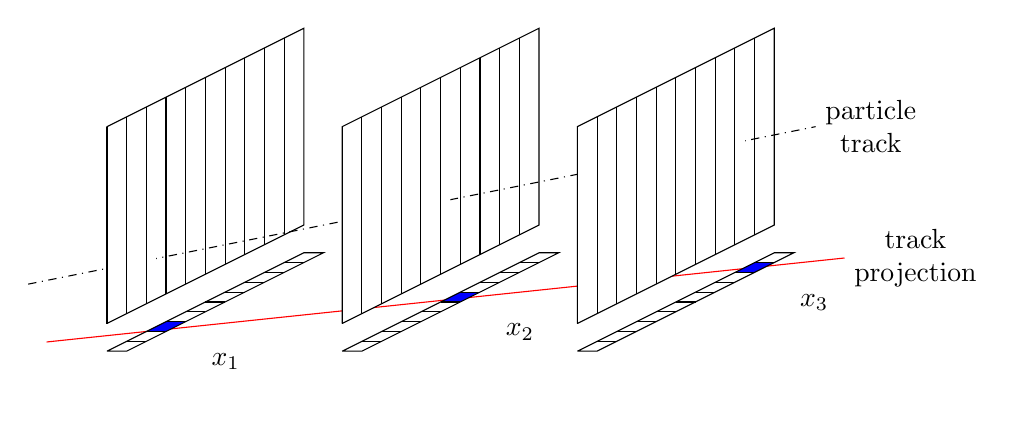
\begin{tikzpicture}[scale=.5,every node/.style={minimum size=1cm},on grid,every text node part/.style={align=center}]
  
% % track
\begin{scope}
 \draw[dashdotted] (-2,1) -- (18,5) node[right] {particle\\track};
\end{scope}

 % projection
\begin{scope}[ yshift=-20, xslant=2]
  \draw[,domain=-2:14,variable=\x,red] plot ({\x},{0.5+2.0/15.0*\x})  node[right,black] {track\\projection};
\end{scope}

% modules
\begin{scope}[ yslant=0., yslant=0.5]
 \draw[draw=none,fill=white] (0,0) rectangle ({2*.5+.25},5);
\draw (0,0) -- (0,5) -- (5,5) -- (5,0) -- (0,0);
\foreach \i in {0,1,...,9}
\draw ({.5*\i},0) -- ( {.5*\i},5) ;
\end{scope}

\begin{scope}[ xshift = 170, yslant=0.5]
 \draw[draw=none,fill=white] (0,0) rectangle ({5*.5+.25},5);
  \draw (0,0) -- (0,5) -- (5,5) -- (5,0) -- (0,0);
  \foreach \i in {0,1,...,9}
  \draw ({.5*\i},0) -- ( {.5*\i},5) ;
\end{scope}

\begin{scope}[ xshift = 340, yslant=0.5]
  \draw[draw=none,fill=white] (0,0) rectangle ({8*.5+.25},5);
  \draw (0,0) -- (0,5) -- (5,5) -- (5,0) -- (0,0);
  \foreach \i in {0,1,...,9}
  \draw ({.5*\i},0) -- ( {.5*\i},5) ;
\end{scope}


\begin{scope}[ yshift=-20, xslant=2]
    \fill [blue] (0,{2*.25}) rectangle (.5,{(2+1)*.25}) node [below right, black] {$x_1$};
    \draw (0,0) -- (.5,0) -- (.5,2.5) -- (0,2.5) -- (0,0);
    \foreach \i in {1,...,9}
    \draw (0,{.25*\i},0) -- (0.5,{.25*\i}) ;
  \end{scope}

 \begin{scope}[ xshift = 170, yshift=-20, xslant=2]
    \fill [blue] (0,{5*.25}) rectangle (.5,{(5+1)*.25}) node [below right, black] {$x_2$};
   \draw (0,0) -- (.5,0) -- (.5,2.5) -- (0,2.5) -- (0,0);
   \foreach \i in {1,...,9}
   \draw (0,{.25*\i},0) -- (0.5,{.25*\i}) ;
 \end{scope}

 \begin{scope}[ xshift = 340, yshift=-20, xslant=2]
    \fill [blue] (0,{8*.25}) rectangle (.5,{(8+1)*.25}) node [below right, black] {$x_3$};
   \draw (0,0) -- (.5,0) -- (.5,2.5) -- (0,2.5) -- (0,0);
   \foreach \i in {1,...,9}
   \draw (0,{.25*\i},0) -- (0.5,{.25*\i}) ;
 \end{scope}


\end{tikzpicture}

\caption{{\it A particle crossing the detector and its projection}}\label{tikz:track_reconstruction}
\end{figure}
The impact parameter resolution depends not only on the intrinsic sensor
resolution but also on the precise alignment of the whole detector and on the
multiple scattering of the materials. These
parameters can be optimised independently in order to achieve the best
resolution. The optimisation follows a two steps procedure:
\begin{itemize}
\item optimisation of the planes alignment;
\item optimisation of the impact point detection.
\end{itemize}


%In the first part of the analysis only the events with a single clusters were
%used, since they can be associated associated with the track produced by a
%unique particle. Once we have fully carachterised the detectors we will explore
%multi-particle track reconstruction.

\subsection{The alignment procedure}
Even though built with high precision, in a detector system with multiple
modules some misalignment between the modules can happen
(\fig{fig:module_misalignment}). In order not to introduce a systematic bias
while evaluating the system resolution it is necessary to align all the modules
to a reference frame (\fig{fig:module_alignment}) introducing an offset in the coordinate system for each module.\\
\begin{figure}[!htbp]
  \centering 
  \subfloat[] { 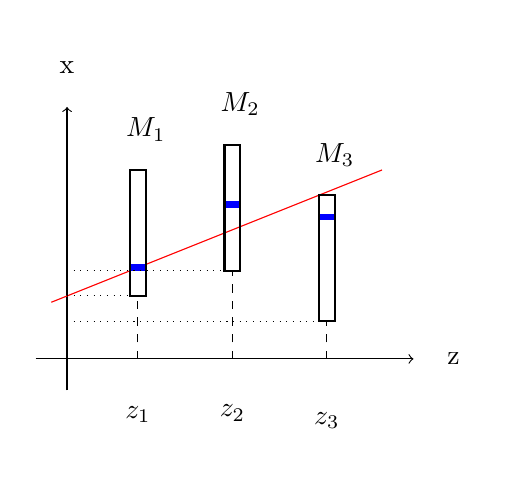
\begin{tikzpicture}[scale=.4,every node/.style={minimum size=1cm},on grid,every
  text node part/.style={align=center}, declare function={ track(\x) = 1.+3.0/7.5*\x; }]

  % original, misaligned
  \def \a {0}
  \def \b {.8}
  \def \c {-.8}

  \begin{scope}
    % axis
    \draw[->] (-1,-1) -- (11,-1) node[right] {z};
    \draw[->] (0,-2) -- (0,7) node[above] {x};

    % track
    \draw[,domain=-.5:10,variable=\x,red] plot ({\x}, {track(\x)} );

    % m1
    \draw[dashed] (2.25,-1) -- (2.25,1) node[below=1] {$z_1$};
    \fill[blue] (2,{track(2)+\a}) rectangle (2.5,{track(2.5) +\a});
    \draw[dotted] (0,1) -- (2,1);
    \draw[thick] (2,{1 +\a}) rectangle (2.5,{5 +\a})  node[above] {$M_1$};
    
    % m2
    \draw[dashed] (5.25,-1) -- (5.25,{1+\b}) node[below=1.3] {$z_2$};
    \fill[blue]  (5,{track(5) +\b}) rectangle (5.5,{track(5.5) +\b});
    \draw[dotted] (0,{1+\b}) -- (5,{1+\b});
    \draw[thick] (5,{1 +\b})          rectangle (5.5,{5 +\b})  node[above] {$M_2$};
    
    % m3
    \draw[dashed] (8.25,-1) -- (8.25,{1+\c}) node[below=.75] {$z_3$};
    \fill[blue]  (8,{track(8) +\c}) rectangle (8.5,{track(8.5) +\c});
    \draw[dotted] (0,{1+\c}) -- (8,{1+\c});
    \draw[thick] (8,{1 +\c})          rectangle (8.5,{5 +\c})  node[above] {$M_3$};
  \end{scope}
  
\end{tikzpicture}
 \label{fig:module_misalignment}}
  \subfloat[] { 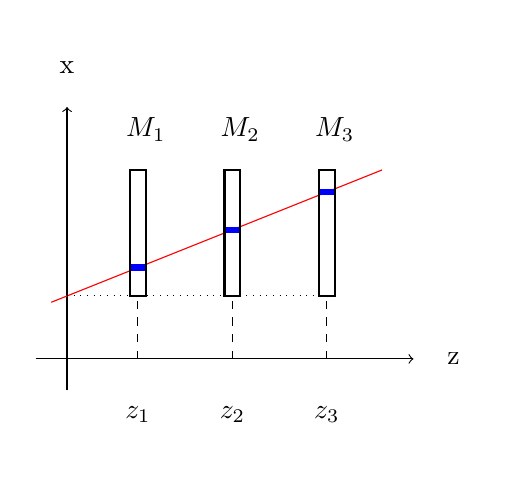
\begin{tikzpicture}[scale=.4,every node/.style={minimum size=1cm},on grid,every
  text node part/.style={align=center}, declare function={ track(\x) = 1.+3.0/7.5*\x; }]

  % original, misaligned
  \def \a {0}
  \def \b {.8}
  \def \c {-.8}


  % original, aligned
  \begin{scope}
    % axis
    \draw[->] (-1,-1) -- (11,-1) node[right] {z};
    \draw[->] (0,-2) -- (0,7) node[above] {x};

    % track
    \draw[,domain=-.5:10,variable=\x,red] plot ({\x}, {track(\x)} );

    % m1
    \draw[dashed] (2.25,-1) -- (2.25,1) node[below=1] {$z_1$};

    \fill[blue] (2,{track(2)}) rectangle (2.5,{track(2.5)});
    \draw[thick] (2,1) rectangle (2.5,5)  node[above] {$M_1$};
    
    % m2
    \draw[dashed] (5.25,-1) -- (5.25,1) node[below=1] {$z_2$};
    \fill[blue]  (5,{track(5)}) rectangle (5.5,{track(5.5)});
    \draw[thick] (5,1)          rectangle (5.5,5)  node[above] {$M_2$};
    
    % m3
    \draw[dashed] (8.25,-1) -- (8.25,1) node[below=1] {$z_3$};
    \fill[blue]  (8,{track(8)}) rectangle (8.5,{track(8.5)});
    \draw[dotted] (0,{1}) -- (8,{1});
    \draw[thick] (8,1)          rectangle (8.5,5)  node[above] {$M_3$};
  \end{scope}

  
\end{tikzpicture}
 \label{fig:module_alignment}}
  \caption{ \it Small misalignments between detector modules that affect the
    track reconstruction cannot be avoided (a) when building the detector. A
    software procedure can effectively improve the alignment. In all the
    following figures $z$ represents the position along the beam axis.
%  \caption{\it {In the ideal case (a) the modules are perfectly aligned: in blue
%      the expected hit points. In the real world nevertheless the exact
%      alignment isn't achievable (b): the particle traverse the detector in slightly
%      different positions.}
  }\label{tikz:module_alignment}
\end{figure}
The zero step required to align the system is to select one of the modules as
the absolute reference frame: all the remaining modules will be aligned with
respect to it. In the following module $M_1$ (\fig{tikz:module_alignment}) will
be taken as the reference. The alignment procedure has been performed with the
detector perpendicularly aligned with respect to the beam axis in such a way
that the distribution of angular coefficients of the tracks is symmetric around
zero.\\
\begin{figure}[!htbp]
  \centering 
  \subfloat[] { \begin{tikzpicture}[scale=.4,every node/.style={minimum size=1cm},on grid,every
  text node part/.style={align=center}, declare function={ track(\x) =
    1.+3.0/7.5*\x; trackb(\x) = 1.9+.4/1.5*(\x-2.25); }]
  
  \def \a {.0}
  \def \c {-.8}

  % misaligned 
  \begin{scope}
    % axis
     \draw[->] (-1,-1) -- (11,-1) node[right] {z};
    \draw[->] (0,-2) -- (0,7) node[above] {x};

    % angle & track
    \shade[left color=white,right color=red!50!white ] (3.5,{trackb(3.5)}) --
    ({3.5+2},{trackb(3.5)}) arc (0:14.9:2)  -- cycle ;
    \draw[red] (3.5,{trackb(3.5)}) -- (6.5,{trackb(3.5)})  node[below left] {$\alpha$};
    \draw[red,domain=-.5:10,variable=\x] plot ({\x}, {trackb(\x)} ) ;

    % m1
    \draw[dashed] (2.25,-1) -- (2.25,{1+\a}) node[below=1] {$z_1$};
    \draw[dashed] (2.25,{track(2.25)} ) -- (0,{track(2.25)}) node[left] {$x_1$};
    \fill[blue] (2,{track(2)+\a}) rectangle (2.5,{track(2.5) +\a});
    \draw[thick] (2,{1 +\a}) rectangle (2.5,{5 +\a})  node[above] {$M_1$};
    
    % m3
    \draw[dashed] (8.25,-1) -- (8.25,{1+\c}) node[below=.75] {$z_3$};
    \draw[dashed] (8,{track(8.25) +\c} ) -- (0,{track(8.25) +\c}) node[left] {$x_3$};    
    \fill[blue]  (8,{track(8) +\c}) rectangle (8.5,{track(8.5) +\c});
    \draw[thick] (8,{1 +\c})          rectangle (8.5,{5 +\c})  node[above] {$M_3$};
  \end{scope}


\end{tikzpicture}
 \label{fig:align13_a}}
  \subfloat[] { 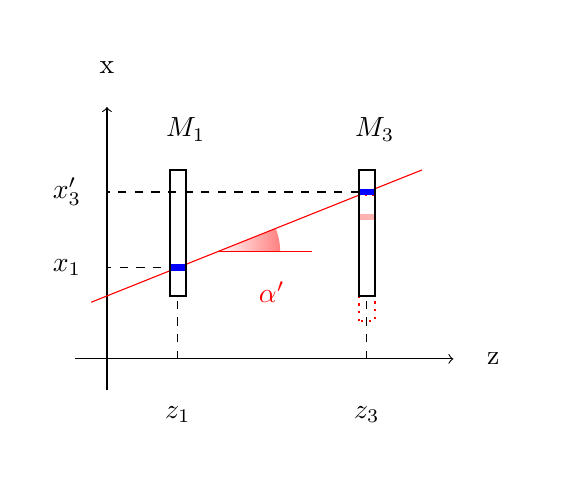
\begin{tikzpicture}[scale=.4,every node/.style={minimum size=1cm},on grid,every
  text node part/.style={align=center}, declare function={ track(\x) =
    1.+3.0/7.5*\x; trackb(\x) = 1.9+.4/1.5*(\x-2.25); }]
  
  \def \a {.0}
  \def \c {-.8}

  % aligned
  \begin{scope}
    % axis
     \draw[->] (-1,-1) -- (11,-1) node[right] {z};
    \draw[->] (0,-2) -- (0,7) node[above] {x};

    % angle & track
    \shade[left color=white,right color=red!50!white ] (3.5,{track(3.5)}) --
    ({3.5+2},{track(3.5)}) arc (0:21.8:2)  -- cycle;
    \draw[red] (3.5,{track(3.5)}) -- (6.5,{track(3.5)})  node[below left] {$\alpha'$};
    \draw[red,domain=-.5:10,variable=\x] plot ({\x}, {track(\x)} );

    % m1
    \draw[dashed] (2.25,-1) -- (2.25,1) node[below=1] {$z_1$};
    \draw[dashed] (2.25,{track(2.25)} ) --  (0,{track(2.25)}) node[left] {$x_1$};
    \fill[blue] (2,{track(2)}) rectangle (2.5,{track(2.5)});
    \draw[thick] (2,1) rectangle (2.5,5)  node[above] {$M_1$};
        
    % m3
    \draw[dashed] (8,{track(8.25)} ) -- (0,{track(8.25)}) node[left] {$x_3'$};    
    \draw[dashed] (8.25,-1) -- (8.25,1) node[below=1] {$z_3$};

    \fill[red!30!white]  (8,{track(8) +\c}) rectangle (8.5,{track(8.5) +\c});
    \draw[thick,dotted,red] (8,{1 +\c})          rectangle (8.5,{5 +\c});

    \fill[blue]  (8,{track(8)}) rectangle (8.5,{track(8.5)});
    \draw[thick] (8,1)          rectangle (8.5,5)  node[above] {$M_3$};
  \end{scope}
  
\end{tikzpicture}
 \label{fig:align13_b}} 
  \caption{\it If the modules are aligned the angular distribution of the tracks
    $\tan{\alpha}$ has to be symmetrical around 0, but this (a) is usually not
    the case. The introduction of the software alignment (\eq{eq:correzione3})
    allows to restore the correct alignement (b).}
  \label{fig:align13}
\end{figure} 
Using modules $M_1$ and $M_3$ (\fig{fig:align13}), the
angular coefficient for each (1-cluster) track is computed:
\begin{equation}\label{eq:m13}
m_{1,3} = \frac{x_3-x_1}{z_3-z_1} = \tan{(\alpha)}
\end{equation}
$x_1$ and $x_3$ being the impact point on $M_1$ and $M_3$ respectively, and $z_1$
and $z_3$ the position along the beam axis.  If the detectors are not perfectly
aligned the initial distribution is not centered around zero
(\fig{fig:align13_a}). This effect can be corrected (\fig{fig:align13_b})
introducing an offset $\Delta_3$ so that
\begin{eqnarray}
x_3' & = & x_3 + \Delta_3 \label{eq:correzione3}\\
m'_{1,3} &=& \frac{x'_3-x_1}{z_3-z_1} = \tan{(\alpha')}\label{eq:m13corretta}
\end{eqnarray}
\begin{figure}[!htbp]
  \centering 
  \subfloat[] { \includegraphics[width=0.5\textwidth]{cap4/immagini/before_align3.jpg} }
  \subfloat[] { \includegraphics[width=0.5\textwidth]{cap4/immagini/after_align3.jpg} }\\
  \caption{ {\it Angular distribution of the tracks before (a) and after (b) the
    alignment procedure.}}
  \label{fig:tan_alpha}
\end{figure}
The angular coefficient distribution is recomputed using \eq{eq:m13corretta}:
\fig{fig:tan_alpha} shows the result.\\
\begin{figure}[!htbp]
  \centering 
  \subfloat[] { 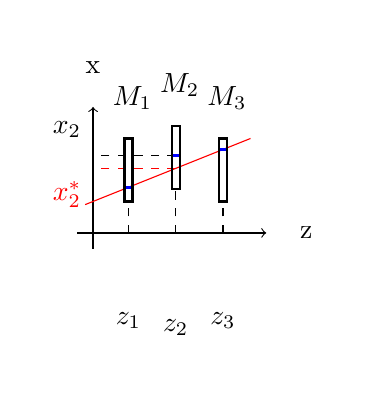
\begin{tikzpicture}[scale=.2,every node/.style={minimum size=1cm},on grid,every
  text node part/.style={align=center}, declare function={ track(\x) =
    1.+3.0/7.5*\x; trackb(\x) = 1.9+.4/1.5*(\x-2.25); }]
  
  \def \a {.0}
  \def \b {.8}

  % misaligned 
  \begin{scope}
   % axis
    \draw[->] (-1,-1) -- (11,-1) node[right] {z};
    \draw[->] (0,-2) -- (0,7) node[above] {x};

    % angle & track
    \draw[red,domain=-.5:10,variable=\x] plot ({\x}, {track(\x)} ) ;
    \draw[dashed,red] (5.25,{track(5.25)} ) --  (0,{track(5.25)}) node[below
    left = -.25] {$x_2^*$};

    % m1
%    \draw[dashed] (2.25,{track(2.25)} ) --  (0,{track(2.25)}) node[left] {$x_1$};
    \draw[dashed] (2.25,-1) -- (2.25,1) node[below=1] {$z_1$};
    \fill[blue] (2,{track(2)}) rectangle (2.5,{track(2.5)});
    \draw[thick] (2,1) rectangle (2.5,5)  node[above] {$M_1$};
    

    % m2
    \draw[dashed] (5.25,{track(5.25)+\b} ) --  (0,{track(5.25)+\b}) node[above left=-.25] {$x_2$};
    \draw[dashed] (5.25,-1) -- (5.25,{1+\b}) node[below=1.25] {$z_2$};
    \fill[blue] (5,{track(5)+\b}) rectangle (5.5,{track(5.5)+\b});
    \draw[thick] (5,{1+\b}) rectangle (5.5,{5+\b})  node[above] {$M_2$};

    % m3
%    \draw[dashed] (8,{track(8.25)} ) -- (0,{track(8.25)}) node[left] {$x_3$};    
    \draw[dashed] (8.25,-1) -- (8.25,1) node[below=1] {$z_3$};
    \fill[blue]  (8,{track(8)}) rectangle (8.5,{track(8.5)});
    \draw[thick] (8,1)          rectangle (8.5,5)  node[above] {$M_3$};

  \end{scope}

  
\end{tikzpicture}
 \label{fig:align2_a} }
  \subfloat[] { \begin{tikzpicture}[scale=.4,every node/.style={minimum size=1cm},on grid,every
  text node part/.style={align=center}, declare function={ track(\x) =
    1.+3.0/7.5*\x; trackb(\x) = 1.9+.4/1.5*(\x-2.25); }]
  
  \def \a {.0}
  \def \b {.8}

  % aligned
  \begin{scope} [xshift = 520]

   % axis
    \draw[->] (-1,-1) -- (11,-1) node[right] {z};
    \draw[->] (0,-2) -- (0,7) node[above] {x};

    % track
    \draw[red,domain=-.5:10,variable=\x] plot ({\x}, {track(\x)} ) ;

    % m1
%    \draw[dashed] (2.25,{track(2.25)} ) --  (0,{track(2.25)}) node[left] {$x_1$};
    \draw[dashed] (2.25,-1) -- (2.25,1) node[below=1] {$z_1$};
    \fill[blue] (2,{track(2)}) rectangle (2.5,{track(2.5)});
    \draw[thick] (2,1) rectangle (2.5,5)  node[above] {$M_1$};
    

    % m2

    \fill[red!50!white] (5,{track(5)+\b}) rectangle (5.5,{track(5.5)+\b});
    \draw[thick,red,dotted] (5,{1+\b}) rectangle (5.5,{5+\b});


    \draw[dashed] (5.25,{track(5.25)} ) --  (0,{track(5.25)}) node[left] {$x_2'=x_2+\Delta_2$};
    \draw[dashed] (5.25,-1) -- (5.25,{1}) node[below=1] {$z_2$};
    \fill[blue] (5,{track(5)}) rectangle (5.5,{track(5.5)});
    \draw[thick] (5,1) rectangle (5.5,5)  node[above] {$M_2$};

    % m3
%    \draw[dashed] (8,{track(8.25)} ) -- (0,{track(8.25)}) node[left] {$x_3$};    
    \draw[dashed] (8.25,-1) -- (8.25,1) node[below=1] {$z_3$};
    \fill[blue]  (8,{track(8)}) rectangle (8.5,{track(8.5)});
    \draw[thick] (8,1)          rectangle (8.5,5)  node[above] {$M_3$};
  \end{scope}
  
\end{tikzpicture}
 \label{fig:align2_b} }
  \caption{\it Due to the detector misalignment the impact point $x_2$ and the
    reconstructed position $x_2^*$ differs (a). An offset $\Delta_2$ has to be
    introduced to remove the systematic error (b).}
  \label{fig:align2}
\end{figure} 
Using $m'_{1,3}$ it is
possible to estimate the theoretical impact point $x_2^*$ on $M_2$ (\fig{fig:align2_a}):
\begin{equation}\label{eq:x2_teorico}
x_2^* = m'_{1,3}\cdot z_2 + x_1
\end{equation}
Such a value can be used to estimate the misalignment of $M_2$ computing the
distribution of the {\em residuals} i.e. the difference between the estimated
point $x_2^*$ and the actual impact point $x_2$:
\begin{equation}
{\rm res}_2 = x_2-x_2^*
\end{equation}

\begin{figure}[!htbp]
  \centering 
  \subfloat[] { \includegraphics[width=0.5\textwidth]{cap4/immagini/before_align2.jpg} }
  \subfloat[] { \includegraphics[width=0.5\textwidth]{cap4/immagini/after_align2.jpg} }\\
  \caption{ {\it Distribution of the residuals before (a) and after (b) the
      software alignment procedure.}}
  \label{fig:tan_alpha}
\end{figure}

\fig{fig:residui} shows an example of such a distribution. The mean value of the
residual distribution $\Delta_2$ can be used as an offset to correct for the
misalignment (\fig{fig:align2_b}):
\begin{equation}
x_2'  =  x_2 + \Delta_2
\end{equation}
The new determined impact points ($x_1$,$z_1$),($x_2'$,$z_2$),($x_3'$,$z_3$) can be
finally used to reconstruct the particle trajectory via a linear fit.


\subsection{The $\eta$ correction}\label{sect:eta_correction}
As shown in section~\ref{subs:cluster} the use of the center of gravity
method~\eq{eq:cog} to estimate the particle impact point is biased due to
charge sharing effect. Considering a two-strip cluster, for example, it is
possible to write the reconstructed hit point $x_{cm}$ in terms of the $\eta$ quantity:
\begin{equation}\label{eq:cm_eta}
x_{cm} = x_L+p \left(1+\eta\right)
\end{equation}
where $x_L$ is the position of the left strip and $p$ the strip pitch.\\
It is trivial to verify that if $\eta=-1(1)$ the left (right) strip collected
the whole charge and $x_{cm} = x_{L(R)}$ while if $\eta=0$ the charge is equally
shared, corresponding to a particle in the middle ($x_{cm} =
x_{L}+p/2$). \fig{fig:interstrip_biased} shows in fact that the interstrip
distribution agrees with the $\eta$ distribution (\fig{}).\\
The nonlinearity in the charge sharing results in a systematic shift in the
reconstructed hit position that in turn worsen the estimation of the detector
spatial resolution.\\
In order to correct the reconstructed position a dedicated procedure is
required. A more general form of~\eq{cm-eta} is
\begin{equation}\label{eq:eta_correction}
x_{\rm pos} = x_L+f(\eta) \cdot p
\end{equation}
with $f(\eta)$ satisfying the following conditions:
\begin{itemize}
\item if the whole charge is collected on the left strip $\eta=-1$ and $x_{\rm
    pos} = x_L$ requires that $f(-1)=0$;
\item if the whole charge is collected on the right strip $\eta=1$, and $x_{\rm
    pos} = x_L+p = x_R$ requires that $f(1)=1$;
\item if the same fraction of the charge is collected on the two strips $\eta=0$
  and $x_{\rm pos} = x_L+p/2 = (x_L + x_R)/2$ requires that $f(0) = 1/2$.
\end{itemize}
Due to the non-linearity of the charge diffusion $f(\eta)$ has to be non-linear
too. A further condition is
\begin{itemize}
\item $f(\eta)$ has to be strictly increasing.
\end{itemize}
Among all the possible choices of function that satisfy the following requests,
the function which produces the systematically correct impact point is
the cumulative probability distribution function of
$\eta$~\cite{Turchetta:1993vu}:
\begin{equation}\label{eq:f_eta}
  f(\eta)= \frac{\int_{-1}^{\eta} \left({\rm d} N/{\rm d} \eta'\right) d\eta' }{\int_{-1}^{1} \left({\rm d} N/{\rm d} \eta'\right) d\eta'}
\end{equation}
$\left({\rm d} N/{\rm d} \eta\right)$ being the experimental $\eta$
distribution. The method, known as the $\eta$ algorithm, consists in the
following steps:
\begin{enumerate}
\item compute the $\eta$ distribution for each module considering only events
  with a single two-strip cluster~\fig{fig:eta_2_strip};
\item compute the interstrip position, defined as the particle hit position rescaled to
  the strip pitch~\fig{fig:interstrip};
\item using \eq{eq:f_eta} and \eq{eq:eta_correction} compute the correct particle position on each module;
\item recompute the corrected interstrip position has been recomputed using
  $x_{\rm pos}$;
\item {\color{red} the increase in the spatial resolution value has been
    ascribed to the eta algorithm itself which introduces a further dependence
    on the position\ldots }
\end{enumerate}
The new interstrip distribution is expected to be flatter than the one computed
using $x_{cm}$ showing that he dependence of the recontructed position from the impact
position inside the strip has been removed. The effect of this procedure on the
spatial resolution of the detector will be discussed in
section~\ref{sect::spatial_resolution}.

\section{Track reconstruction}
In case of one hit per module there is no ambiguity in the track reconstruction:
the impact position is defined using the $\eta$ algorithm and its
indetermination is given by the resolution of the corresponding detector. A
fit of the expected trajectory gives the relevant informations.\\
If different particles are detected in the same event though, the procedure can
be cumbersome: the different hit points can be due to different particles,
secondary particles can be generated,
a module can miss the detection of a particle,\ldots and a careful reconstruction procedure is required.\\
Many algorithms for finding and fitting particle tracks have been developed:
least square methods, filters, adaptive methods and so on. In this thesis work a
simple least square fit to reconstruct tracks has been used and only the events
in which all the detector modules detect the same number of clusters have been
considered, given only three
points are available. \\
The track reconstruction algorithm consists of two procedures. The first
procedure is the {\em track finding}, i.e. the estimate of the set of possible
track candidates. Despite the fact that the track finding should be very
conservative in order not to reject possible solutions, the fact that the
particles travel in a straight line allows to reduce the number of track
candidates. The procedure is the following:
\begin{enumerate}
\item for each $x_1^{(i)}\in M_1$ and for each  $x_3^{(j)}\in M_3$ construct the
  pair $\{x_1^{(i)},x_3^{(j)}\}$;
\item if $\exists x_2^{(k)}\in M_2$ that lies in the straight line between
  $x_1^{(i)}$ and $x_3^{(j)}$ within errors, then the points $\{x_1^{(i)},x_2^{(k)},x_3^{(j)}\}$
  define a possible candidate (\fig{fig:track_candidates_ok});
\item if $\nexists x_2^{(k)}\in M_2$ that satisfies the above condition (\fig{fig:track_candidates_nok}) discard
  the pair $\{x_1^{(i)},x_3^{(j)}\}$. 
\end{enumerate}
\begin{figure}[!htbp]
  \centering 
  \subfloat[]{ 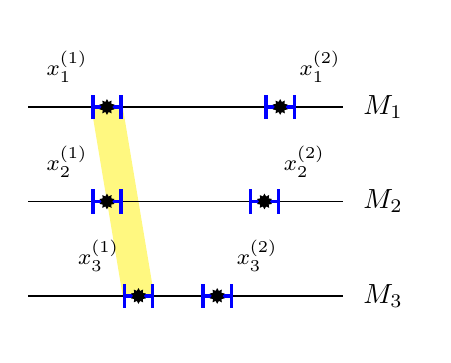
\begin{tikzpicture}[scale=.4,every node/.style={minimum size=1cm},on grid,every
  text node part/.style={align=center}, declare function={ track(\x) =
    1.+3.0/7.5*\x; trackb(\x) = 1.9+.4/1.5*(\x-2.25); }]
  
  \def \a {2.5}
  \def \b {8}

  \begin{scope}

    \fill[yellow!50!white] (2,6) -- (3,0) -- (4,0) -- (3,6);
    
    \def \y {6}
    \draw (0,\y) -- (10,\y) node[right] {$M_1$};
    \draw[blue,very thick,|-|] ({2.5-.5},\y) -- ({2.5+.5},\y);
    \node[fill,star,star points=10,scale=0.2] (x11) at (2.5,\y) {} node[above left] at
    (x11) {\footnotesize $x_1^{(1)}$};
    \draw[blue,very thick,|-|] ({8-.5},\y) -- ({8+.5},\y);
    \node[fill,star,star points=10,scale=0.2] (x12) at (8,\y) {} node[above right] at
    (x12) {\footnotesize $x_1^{(2)}$};

    \def \y {3}
    \draw (0,\y) -- (10,\y) node[right] {$M_2$};
    \draw[blue,very thick,|-|] ({2.5-.5},\y) -- ({2.5+.5},\y);
    \node[fill,star,star points=10,scale=0.2] (x21) at (2.5,\y) {} node[above left] at
    (x21) {\footnotesize $x_2^{(1)}$};
    \draw[blue,very thick,|-|] ({7.5-.5},\y) -- ({7.5+.5},\y);
    \node[fill,star,star points=10,scale=0.2] (x22) at (7.5,\y) {} node[above right] at
    (x22) {\footnotesize $x_2^{(2)}$};

    \def \y {0}
    \draw (0,\y) -- (10,\y) node[right] {$M_3$};
    \draw[blue,very thick,|-|] ({3.5-.5},\y) -- ({3.5+.5},\y);
    \node[fill,star,star points=10,scale=0.2] (x31) at (3.5,\y) {} node[above left] at
    (x31) {\footnotesize $x_3^{(1)}$};
    \draw[blue,very thick,|-|] ({6-.5},\y) -- ({6+.5},\y);
    \node[fill,star,star points=10,scale=0.2] (x32) at (6,\y) {} node[above right] at
    (x32) {\footnotesize $x_3^{(2)}$};
    

  \end{scope}


\end{tikzpicture}
 \label{fig:track_candidates_ok} }\quad
  \subfloat[]{ 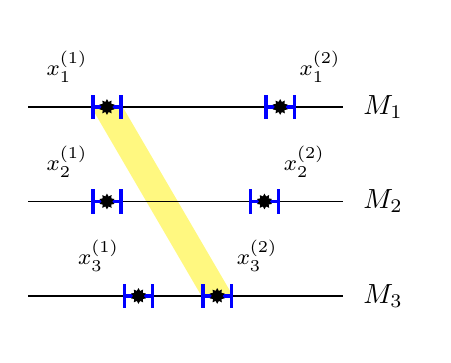
\begin{tikzpicture}[scale=.4,every node/.style={minimum size=1cm},on grid,every
  text node part/.style={align=center}, declare function={ track(\x) =
    1.+3.0/7.5*\x; trackb(\x) = 1.9+.4/1.5*(\x-2.25); }]
  
  \def \a {2.5}
  \def \b {8}


  \begin{scope}%[xshift = 520]

    \fill[yellow!50!white] (2,6) -- (5.5,0) -- (6.5,0) -- (3,6);
      
    
    \def \y {6}
    \draw (0,\y) -- (10,\y) node[right] {$M_1$};
    \draw[blue,very thick,|-|] ({2.5-.5},\y) -- ({2.5+.5},\y);
    \node[fill,star,star points=10,scale=0.2] (x11) at (2.5,\y) {} node[above left] at
    (x11) {\footnotesize $x_1^{(1)}$};
    \draw[blue,very thick,|-|] ({8-.5},\y) -- ({8+.5},\y);
    \node[fill,star,star points=10,scale=0.2] (x12) at (8,\y) {} node[above right] at
    (x12) {\footnotesize $x_1^{(2)}$};

    \def \y {3}
    \draw (0,\y) -- (10,\y) node[right] {$M_2$};
    \draw[blue,very thick,|-|] ({2.5-.5},\y) -- ({2.5+.5},\y);
    \node[fill,star,star points=10,scale=0.2] (x21) at (2.5,\y) {} node[above left] at
    (x21) {\footnotesize $x_2^{(1)}$};
    \draw[blue,very thick,|-|] ({7.5-.5},\y) -- ({7.5+.5},\y);
    \node[fill,star,star points=10,scale=0.2] (x22) at (7.5,\y) {} node[above right] at
    (x22) {\footnotesize $x_2^{(2)}$};

    \def \y {0}
    \draw (0,\y) -- (10,\y) node[right] {$M_3$};
    \draw[blue,very thick,|-|] ({3.5-.5},\y) -- ({3.5+.5},\y);
    \node[fill,star,star points=10,scale=0.2] (x31) at (3.5,\y) {} node[above left] at
    (x31) {\footnotesize $x_3^{(1)}$};
    \draw[blue,very thick,|-|] ({6-.5},\y) -- ({6+.5},\y);
    \node[fill,star,star points=10,scale=0.2] (x32) at (6,\y) {} node[above right] at
    (x32) {\footnotesize $x_3^{(2)}$};

  \end{scope}

%  % aligned
%  \begin{scope} [xshift = 520]
%
%   % axis
%    \draw[->] (-1,-1) -- (11,-1) node[right] {z};
%    \draw[->] (0,-2) -- (0,7) node[above] {x};
%
%    % track
%    \draw[red,domain=-.5:10,variable=\x] plot ({\x}, {track(\x)} ) ;
%
%    % m1
%%    \draw[dashed] (2.25,{track(2.25)} ) --  (0,{track(2.25)}) node[left] {$x_1$};
%    \draw[dashed] (2.25,-1) -- (2.25,1) node[below=1] {$z_1$};
%    \fill[blue] (2,{track(2)}) rectangle (2.5,{track(2.5)});
%    \draw[thick] (2,1) rectangle (2.5,5)  node[above] {$M_1$};
%    
%
%    % m2
%
%    \fill[red!50!white] (5,{track(5)+\b}) rectangle (5.5,{track(5.5)+\b});
%    \draw[thick,red,dotted] (5,{1+\b}) rectangle (5.5,{5+\b});
%
%
%    \draw[dashed] (5.25,{track(5.25)} ) --  (0,{track(5.25)}) node[left] {$x_2'=x_2+\Delta_2$};
%    \draw[dashed] (5.25,-1) -- (5.25,{1}) node[below=1] {$z_2$};
%    \fill[blue] (5,{track(5)}) rectangle (5.5,{track(5.5)});
%    \draw[thick] (5,1) rectangle (5.5,5)  node[above] {$M_2$};
%
%    % m3
%%    \draw[dashed] (8,{track(8.25)} ) -- (0,{track(8.25)}) node[left] {$x_3$};    
%    \draw[dashed] (8.25,-1) -- (8.25,1) node[below=1] {$z_3$};
%    \fill[blue]  (8,{track(8)}) rectangle (8.5,{track(8.5)});
%    \draw[thick] (8,1)          rectangle (8.5,5)  node[above] {$M_3$};
%  \end{scope}
%  
\end{tikzpicture}
 \label{fig:track_candidates_nok} }
  \caption{\it Pictorial representation of the impact points generated by a two
    particle events on the three modules. The stars represent the detected hit
    points and in blue the position within errors. If the same particle produced
    $x_1$ and $x_3$ we expect to register signal in the shaded area (a) of
    $M_2$, whereas if the points belong to a different particle we expect no
    signal recorded (b).}
  \label{fig:track_candidates}
\end{figure} 
In order to keep the procedure conservative the condition (2) can be modified
requiring $x_2^{(k)}$ to lie in the shaded region considering an error
$s\sigma_2$, where $\sigma_2$ is the spatial resolution of $M_2$ and $s$ is a
handle that can be tuned to improve the effectiveness of the reconstruction.
%In \ref{par:stability_vs_s} we discuss stability of the procedure
%as a function of $s$.\\
The track finding procedure ends when all the possible candidates have been
evaluated (\fig{fig:track_finding}).\\

The {\em track fitting} procedure consists in removing the wrong candidates and
determining the track parameters.
\begin{figure}[!htbp]
  \centering 
  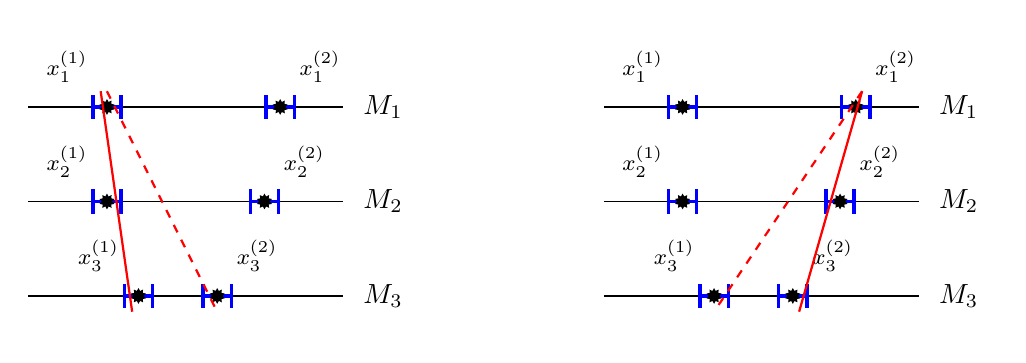
\begin{tikzpicture}[scale=.4,every node/.style={minimum size=1cm},on grid,every
  text node part/.style={align=center}, declare function={ track(\x) =
    1.+3.0/7.5*\x; trackb(\x) = 1.9+.4/1.5*(\x-2.25); }]
  
  \def \a {2.5}
  \def \b {8}

  \begin{scope}

    \def \y {6}
    \draw (0,\y) -- (10,\y) node[right] {$M_1$};
    \draw[blue,very thick,|-|] ({2.5-.5},\y) -- ({2.5+.5},\y);
    \node[fill,star,star points=10,scale=0.2] (x11) at (2.5,\y) {} node[above left] at
    (x11) {\footnotesize $x_1^{(1)}$};
    \draw[blue,very thick,|-|] ({8-.5},\y) -- ({8+.5},\y);
    \node[fill,star,star points=10,scale=0.2] (x12) at (8,\y) {} node[above right] at
    (x12) {\footnotesize $x_1^{(2)}$};

    \def \y {3}
    \draw (0,\y) -- (10,\y) node[right] {$M_2$};
    \draw[blue,very thick,|-|] ({2.5-.5},\y) -- ({2.5+.5},\y);
    \node[fill,star,star points=10,scale=0.2] (x21) at (2.5,\y) {} node[above left] at
    (x21) {\footnotesize $x_2^{(1)}$};
    \draw[blue,very thick,|-|] ({7.5-.5},\y) -- ({7.5+.5},\y);
    \node[fill,star,star points=10,scale=0.2] (x22) at (7.5,\y) {} node[above right] at
    (x22) {\footnotesize $x_2^{(2)}$};

    \def \y {0}
    \draw (0,\y) -- (10,\y) node[right] {$M_3$};
    \draw[blue,very thick,|-|] ({3.5-.5},\y) -- ({3.5+.5},\y);
    \node[fill,star,star points=10,scale=0.2] (x31) at (3.5,\y) {} node[above left] at
    (x31) {\footnotesize $x_3^{(1)}$};
    \draw[blue,very thick,|-|] ({6-.5},\y) -- ({6+.5},\y);
    \node[fill,star,star points=10,scale=0.2] (x32) at (6,\y) {} node[above right] at
    (x32) {\footnotesize $x_3^{(2)}$};

    %tracks
    \draw[red,thick] (2.3,6.5) -- (3.3,-.5);
    \draw[red,thick,dashed] (2.5,6.5) -- (6,-.5);

  \end{scope}



  \begin{scope}[xshift = 520]
    
       \def \y {6}
    \draw (0,\y) -- (10,\y) node[right] {$M_1$};
    \draw[blue,very thick,|-|] ({2.5-.5},\y) -- ({2.5+.5},\y);
    \node[fill,star,star points=10,scale=0.2] (x11) at (2.5,\y) {} node[above left] at
    (x11) {\footnotesize $x_1^{(1)}$};
    \draw[blue,very thick,|-|] ({8-.5},\y) -- ({8+.5},\y);
    \node[fill,star,star points=10,scale=0.2] (x12) at (8,\y) {} node[above right] at
    (x12) {\footnotesize $x_1^{(2)}$};

    \def \y {3}
    \draw (0,\y) -- (10,\y) node[right] {$M_2$};
    \draw[blue,very thick,|-|] ({2.5-.5},\y) -- ({2.5+.5},\y);
    \node[fill,star,star points=10,scale=0.2] (x21) at (2.5,\y) {} node[above left] at
    (x21) {\footnotesize $x_2^{(1)}$};
    \draw[blue,very thick,|-|] ({7.5-.5},\y) -- ({7.5+.5},\y);
    \node[fill,star,star points=10,scale=0.2] (x22) at (7.5,\y) {} node[above right] at
    (x22) {\footnotesize $x_2^{(2)}$};

    \def \y {0}
    \draw (0,\y) -- (10,\y) node[right] {$M_3$};
    \draw[blue,very thick,|-|] ({3.5-.5},\y) -- ({3.5+.5},\y);
    \node[fill,star,star points=10,scale=0.2] (x31) at (3.5,\y) {} node[above left] at
    (x31) {\footnotesize $x_3^{(1)}$};
    \draw[blue,very thick,|-|] ({6-.5},\y) -- ({6+.5},\y);
    \node[fill,star,star points=10,scale=0.2] (x32) at (6,\y) {} node[above right] at
    (x32) {\footnotesize $x_3^{(2)}$};

    % tracks
    \draw[red,thick,dashed] (8.2,6.5) -- (3.5,-.5);
    \draw[red,thick] (8.2,6.5) -- (6.2,-.5);

  \end{scope}


\end{tikzpicture}

  \caption{\it All the track candidates are evaluated. Viable candidates are
    kept (red) while non viable are discarded (dashed red).}
  \label{fig:track_finding}
\end{figure} 
When evaluating the set of all the possible candidates, two cases are possible:
\begin{itemize}
\item the candidates are compatible (\fig{fig:compatible_track}), i.e. on each
  module every hit point belong to a different track;
\item the candidates are incompatible (\fig{fig:incompatible_track}), i.e. at
  least one hit point on one module is part of more than one track.
\end{itemize}
The candidates are rated according the $\chi^2$ goodness of the fit; 
possible incompatible tracks are discarded according the same principle.\\
\begin{figure}[!htbp]
  \centering 
  \subfloat[]{ 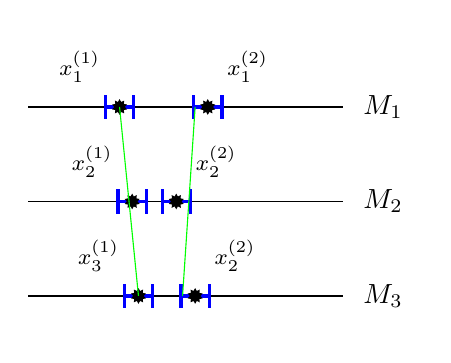
\begin{tikzpicture}[scale=.4,every node/.style={minimum size=1cm},on grid,every
  text node part/.style={align=center}, declare function={ track(\x) =
    1.+3.0/7.5*\x; trackb(\x) = 1.9+.4/1.5*(\x-2.25); }]
  
  \def \a {2.5}
  \def \b {8}

  \begin{scope}

    \def \y {6}
    \draw (0,\y) -- (10,\y) node[right] {$M_1$};
    \def \x {2.9}
    \draw[blue,very thick,|-|] ({\x-.5},\y) -- ({\x+.5},\y);
    \node[fill,star,star points=10,scale=0.2] (x11) at (\x,\y) {} node[above left] at
    (x11) {\footnotesize $x_1^{(1)}$};
    \def \x {5.7}
    \draw[blue,very thick,|-|] ({\x-.5},\y) -- ({\x+.5},\y);
    \node[fill,star,star points=10,scale=0.2] (x12) at (\x,\y) {} node[above right] at
    (x12) {\footnotesize $x_1^{(2)}$};
    
    % M2
    \def \y {3}
    \draw (0,\y) -- (10,\y) node[right] {$M_2$};
    \def \x {3.3}
    \draw[blue,very thick,|-|] ({\x-.5},\y) -- ({\x+.5},\y);
    \node[fill,star,star points=10,scale=0.2] (x21) at (\x,\y) {} node[above left] at
    (x21) {\footnotesize $x_2^{(1)}$};
    \def \x {4.7}
    \draw[blue,very thick,|-|] ({\x-.5},\y) -- ({\x+.5},\y);
    \node[fill,star,star points=10,scale=0.2] (x22) at (\x,\y) {} node[above right] at
    (x22) {\footnotesize $x_2^{(2)}$};
    

    \def \y {0}
    \draw (0,\y) -- (10,\y) node[right] {$M_3$};
    \def \x {3.5}
    \draw[blue,very thick,|-|] ({\x-.5},\y) -- ({\x+.5},\y);
    \node[fill,star,star points=10,scale=0.2] (x31) at (\x,\y) {} node[above left] at
    (x31) {\footnotesize $x_3^{(1)}$};
    \def \x {5.3}
    \draw[blue,very thick,|-|] ({\x-.5},\y) -- ({\x+.5},\y);
    \node[fill,star,star points=10,scale=0.2] (x22) at (\x,\y) {} node[above right] at
    (x22) {\footnotesize $x_2^{(2)}$};

    %tracks
    \draw[green] (2.9,6) -- (3.5,0); % 112
    \draw[green] (5.3,6) -- (4.9,0);

  \end{scope}



\end{tikzpicture}
 \label{fig:compatible_track} }\quad
  \subfloat[]{ 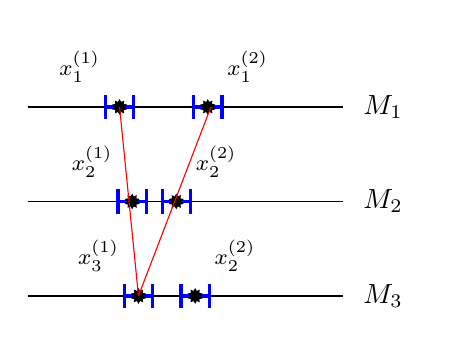
\begin{tikzpicture}[scale=.4,every node/.style={minimum size=1cm},on grid,every
  text node part/.style={align=center}, declare function={ track(\x) =
    1.+3.0/7.5*\x; trackb(\x) = 1.9+.4/1.5*(\x-2.25); }]
  
  \def \a {2.5}
  \def \b {8}



    \begin{scope}

    \def \y {6}
    \draw (0,\y) -- (10,\y) node[right] {$M_1$};
    \def \x {2.9}
    \draw[blue,very thick,|-|] ({\x-.5},\y) -- ({\x+.5},\y);
    \node[fill,star,star points=10,scale=0.2] (x11) at (\x,\y) {} node[above left] at
    (x11) {\footnotesize $x_1^{(1)}$};
    \def \x {5.7}
    \draw[blue,very thick,|-|] ({\x-.5},\y) -- ({\x+.5},\y);
    \node[fill,star,star points=10,scale=0.2] (x12) at (\x,\y) {} node[above right] at
    (x12) {\footnotesize $x_1^{(2)}$};
    
    % M2
    \def \y {3}
    \draw (0,\y) -- (10,\y) node[right] {$M_2$};
    \def \x {3.3}
    \draw[blue,very thick,|-|] ({\x-.5},\y) -- ({\x+.5},\y);
    \node[fill,star,star points=10,scale=0.2] (x21) at (\x,\y) {} node[above left] at
    (x21) {\footnotesize $x_2^{(1)}$};
    \def \x {4.7}
    \draw[blue,very thick,|-|] ({\x-.5},\y) -- ({\x+.5},\y);
    \node[fill,star,star points=10,scale=0.2] (x22) at (\x,\y) {} node[above right] at
    (x22) {\footnotesize $x_2^{(2)}$};
    

    \def \y {0}
    \draw (0,\y) -- (10,\y) node[right] {$M_3$};
    \def \x {3.5}
    \draw[blue,very thick,|-|] ({\x-.5},\y) -- ({\x+.5},\y);
    \node[fill,star,star points=10,scale=0.2] (x31) at (\x,\y) {} node[above left] at
    (x31) {\footnotesize $x_3^{(1)}$};
    \def \x {5.3}
    \draw[blue,very thick,|-|] ({\x-.5},\y) -- ({\x+.5},\y);
    \node[fill,star,star points=10,scale=0.2] (x22) at (\x,\y) {} node[above right] at
    (x22) {\footnotesize $x_2^{(2)}$};

    %tracks
    \draw[red] (2.9,6) -- (3.5,0); % 112
    \draw[red] (5.8,6) -- (3.5,0);

  \end{scope}



\end{tikzpicture}
 \label{fig:incompatible_track} }
  \caption{\it If every hit belong to a sigle track (a) the candidates are
    compatible, whereas if a hit belong to different tracks only the candidate
    with the best $\chi^2$ is considered.}
  \label{fig:track_fitting}
\end{figure} 


{\color{red} questo magari nel capitolo dei multitraccia+calorimetro?}
Before working on multiple particle track reconstruction, single particle events
will be used as a benchmark. The idea beyond this approach is that single
cluster events show no ambiguity, since only one track has to be
reconstructed. The approach is the following:
\begin{itemize}
\item select a couple of single cluster events and determine the trajectory of the
  particles;
\item on each module merge the information on the cluster position from the
  two events;
\item apply the reconstruction algorithm in order to find and fit the two tracks;
\item evaluate the goodness of the algorithm computing how many tracks are
  correctly reconstructed.
\end{itemize}
When discussing the track finding algorithm, a parameter $s$ to tune
the acceptance of the algorithm was introduced. {\color{red} riscrivere This handle affects the goodness of the
algorithm and hat to be carefully tuned in order to maximise the single cluster
acceptance and minimize the benchmark failure.}
{\color{red} Qui un plot per mostrare l'efficienza di ricosruzionein funzione di $s$}




\chapter{Multitrack events with calorimeters}
\label{cap:multitraccia}

\begin{itemize}
\item scopo (breve) e informazioni sui dati
\item descrizione del calorimetro
\item quali passaggi dei precenti abbiamo fatto
\item allineamento e risoluzione
\item tracking eventi singoli
\item multitracking (simulato e reale)
\item risultati
\end{itemize}


Reconstructed tracks have been compared with the outcome of an array of
3$\times$3 SiPM connected to a shashlik electromagnetic calorimeter. Goal of the
activity is to correlate and improve reconstructed hit position with the
calorimeter signal. Before proceeding I will remark some features of
electromagnetic calorimeters that has to be taken into account when analysing
data.\\
When passing trough matter electrons can loose energy because of many different
kind of interaction, nevertheless two main regimes can be identified. At low
energies, below $\sim$10 MeV the energy loss is main due to collision with atoms
and molecules of the material through ionisation and thermal excitation. At
medium energies, $\sim$10 MeV to 1~GeV the main couse of energy loss is
bremsstrahlung. As a consequence electrons of sufficiently high energy
($\geq$1~GeV) incident on a block of material produces secondary photons that can
be in turn converted into an electron-antielectron pair. If these secondary
particles have enough energy the process can continue and give rise to an
electromagnetic cascade. The number or produced particles increase until when
their energy falls below a critical energy 
\begin{equation}\label{eq:critical_energy}
\epsilon \simeq \frac{610 {\rm MeV}}{Z + 1.24}
\end{equation}
thereafter the energy is
released in form of ionisation and excitement.\\
The main features of the electromagnetic shower can be described as a function
of the {\em radiation length} $X_0$, which is characteristic of the material
\cite{pdg}:
\begin{equation}\label{eq:radiation_length}
X_0 \simeq \frac{716 {\rm g\ cm^{-2}}A}{Z(Z+1)\log{287/\sqrt{Z}}}
\end{equation}
where $A$ is the atomic weight and $Z$ the atomic number. The radiation length
represents the depth in the material at which the electron reduce it energy by a
factor $1/e$:
\begin{equation}\label{eq:radiation_length}
\langle E(x) \rangle = E_0 e^{-\frac{x}{X_0}}
\end{equation}
The radiation length and the critical energy can be used to estimate the depth
at which the maximum number of secondary particles is produced:
\begin{equation}\label{eq:shower_max}
t_{\rm max} \simeq \log{\frac{E_0}{\epsilon}} - 0.5
\end{equation}
where $t_{\rm max}$ is measured in radiation lengths and $E_0$ is the incident
particle energy. The calorimeter thickness containing 95\% of the shower energy
is approximately given by
\begin{equation}\label{eq:95tickness}
t_{95\%} \simeq t_{\rm max}+0.08Z+9.6
\end{equation}
$t_{95\%}$ and $t_{\rm max}$ being expressed in radiation lengths.\\
The electromagnetic shower has a transversal spread due to multiple scattering
away from the shower axis and photon bremsstrahlung. A measurement of the
transverse size of the shower at the critical energy is given by the Moli\`ere radius
\begin{equation}\label{eq:moliere_radius}
R_{\rm M} \simeq 21 {\rm MeV} \frac{X_0}{\epsilon}
\end{equation}
Approximately only the 10\% of the shower energy falls outside the cylinder of
radius $\sim 1 R_{\rm M} $


{ \color{red}
%Tracking insede the caloriemters will be done with Si-trackers covering large
%areas with hundreds of channels


}


\chapter{Microstrip silicon detectors for space applications}
\label{cap:gamma400}

In space applications the power consumption is a major issue. Power saving can
be achieved for example reducing as much as possible the number of readout
channel. On the other side reducing the number of readout channels the spatial
resolution is decreased as well.\\
In this part of my research activity I characterised and compared different
readout approaches with respect different layout of the silicon microstrip
sensor. The final goal is to determine the optimal compromise between number of
channels and spatial resolution.


{ \color{red}
\begin{itemize}
\item scopo e informazioni sui dati
\item quali passaggi dei precenti abbiamo fatto
\item allineamento e risoluzione
\item risultati
\end{itemize}
}



\chapter{Medical applications of microstrip silicon detectors}
\label{cap:bnct}

\begin{itemize}
\item scopo e informazioni sui dati
\item quali passaggi dei precenti abbiamo fatto -> questo sottrae gia' il pede
\item risultati
\end{itemize}
}
%\input{cap5/results}

%\begin{appendices}
%\input{appendix/multitrack}
%\end{appendices}
%\input{Tracking/Tracking_SSC_LHC_Sadrozinsky}

%\addcontentsline{toc}{chapter}{List of figures}
%\addcontentsline{toc}{chapter}{List of tables}
\addcontentsline{toc}{chapter}{Bibliography}
\bibliographystyle{unsrt}
\bibliography{biblio/biblio_gre}

%\printnoidxglossaries
%\printglossaries

\end{document}


%%% Local Variables:
%%% mode: latex
%%% TeX-master: t
%%% End:
